% ------------ begin cheatsheet
\documentclass[a4paper]{article}
\usepackage[a4paper,margin=0.1in]{geometry}
\usepackage{multicol}

\usepackage{amsmath, amssymb}
\usepackage[inline]{enumitem}
\usepackage{graphicx}

\usepackage{ulem}
\usepackage{makecell}

% horizontal list
\newlist{hlist}{enumerate*}{1}
\setlist[hlist]{label={}, afterlabel={}, itemjoin={{ \textbar{} }}}

% math
\newcommand{\abs}[1]{\left\lvert#1\right\rvert}
\usepackage{spalign}
\let\mat=\spalignmat
\let\amat=\spalignaugmat

% envs
\newcommand{\oli}[1]{\begin{enumerate*}[label=(\arabic*)]#1\end{enumerate*}}
\newcommand{\red}[1]{\textcolor{red}{#1}}

\graphicspath{ {./images/} }
\pagestyle{empty}
\setlength{\columnseprule}{0.3pt}

% reduce spacing before and after headers
\newcommand{\uppercaseandunderline}[1]{\uline{\uppercase{#1}}}

\makeatletter
\renewcommand{\section}{
  \@startsection{section}{1}{0pt}{1ex}{1.2ex} {\raggedleft\normalfont\large\bfseries\uppercaseandunderline}}
\renewcommand{\subsection}{
  \@startsection{subsection}{2}{0pt}{1ex}{1.2ex} {\raggedleft\normalfont\normalsize\bfseries\fbox}}
\renewcommand{\subsubsection}{
  \@startsection{subsubsection}{3}{0pt}{1ex}{0.8ex} {\raggedleft\normalfont\small\bfseries\uline}}
\renewcommand{\paragraph}{
  \@startsection{paragraph}{4}{0pt}{1.5ex}{-0.8em}{\normalfont\bfseries}}
% ------------ end cheatsheet

% ------------ begin code
\usepackage{xcolor}
\definecolor{dkgreen}{rgb}{0,0.6,0}
\definecolor{gray}{rgb}{0.5,0.5,0.5}
\definecolor{mauve}{rgb}{0.58,0,0.82}
\definecolor{lg}{rgb}{0.9,0.9,0.9}

% code environment
\usepackage{listings}
\lstset{
  %frame=tb, % adds top and bottom border
  aboveskip=1mm,
  belowskip=1mm,
  showstringspaces=false,
  columns=flexible,
  basicstyle={\small\ttfamily},
  numberstyle=\color{gray},
  keywordstyle=\color{blue}\textbf,
  commentstyle=\color{dkgreen},
  stringstyle=\color{mauve},
  breaklines=true,
  breakatwhitespace=true,
  backgroundcolor=\color{lg},
  tabsize=4
}
\newcommand{\ic}[1]{\lstinline{#1}}

% ------------ end code

% SKIPS
% L1 01-29

\begin{document}
\small
\lstset{language=c++}
\setlength{\abovedisplayskip}{0pt}
\setlength{\belowdisplayskip}{0pt}
\setlength{\abovedisplayshortskip}{0pt}
\setlength{\belowdisplayshortskip}{0pt}
\begin{multicols*}{3}
  \part*{\centering \underline{CS3241}}

% --
% PAGE 1
% --

\section*{Intro}
  \subsection*{Image formation}
    \paragraph{Elements}
      \begin{hlist}
        \item Objects
        \item Viewer
        \item Light sources
        \item Materials
      \end{hlist}
    \paragraph{Pinhole camera} \noindent \\
      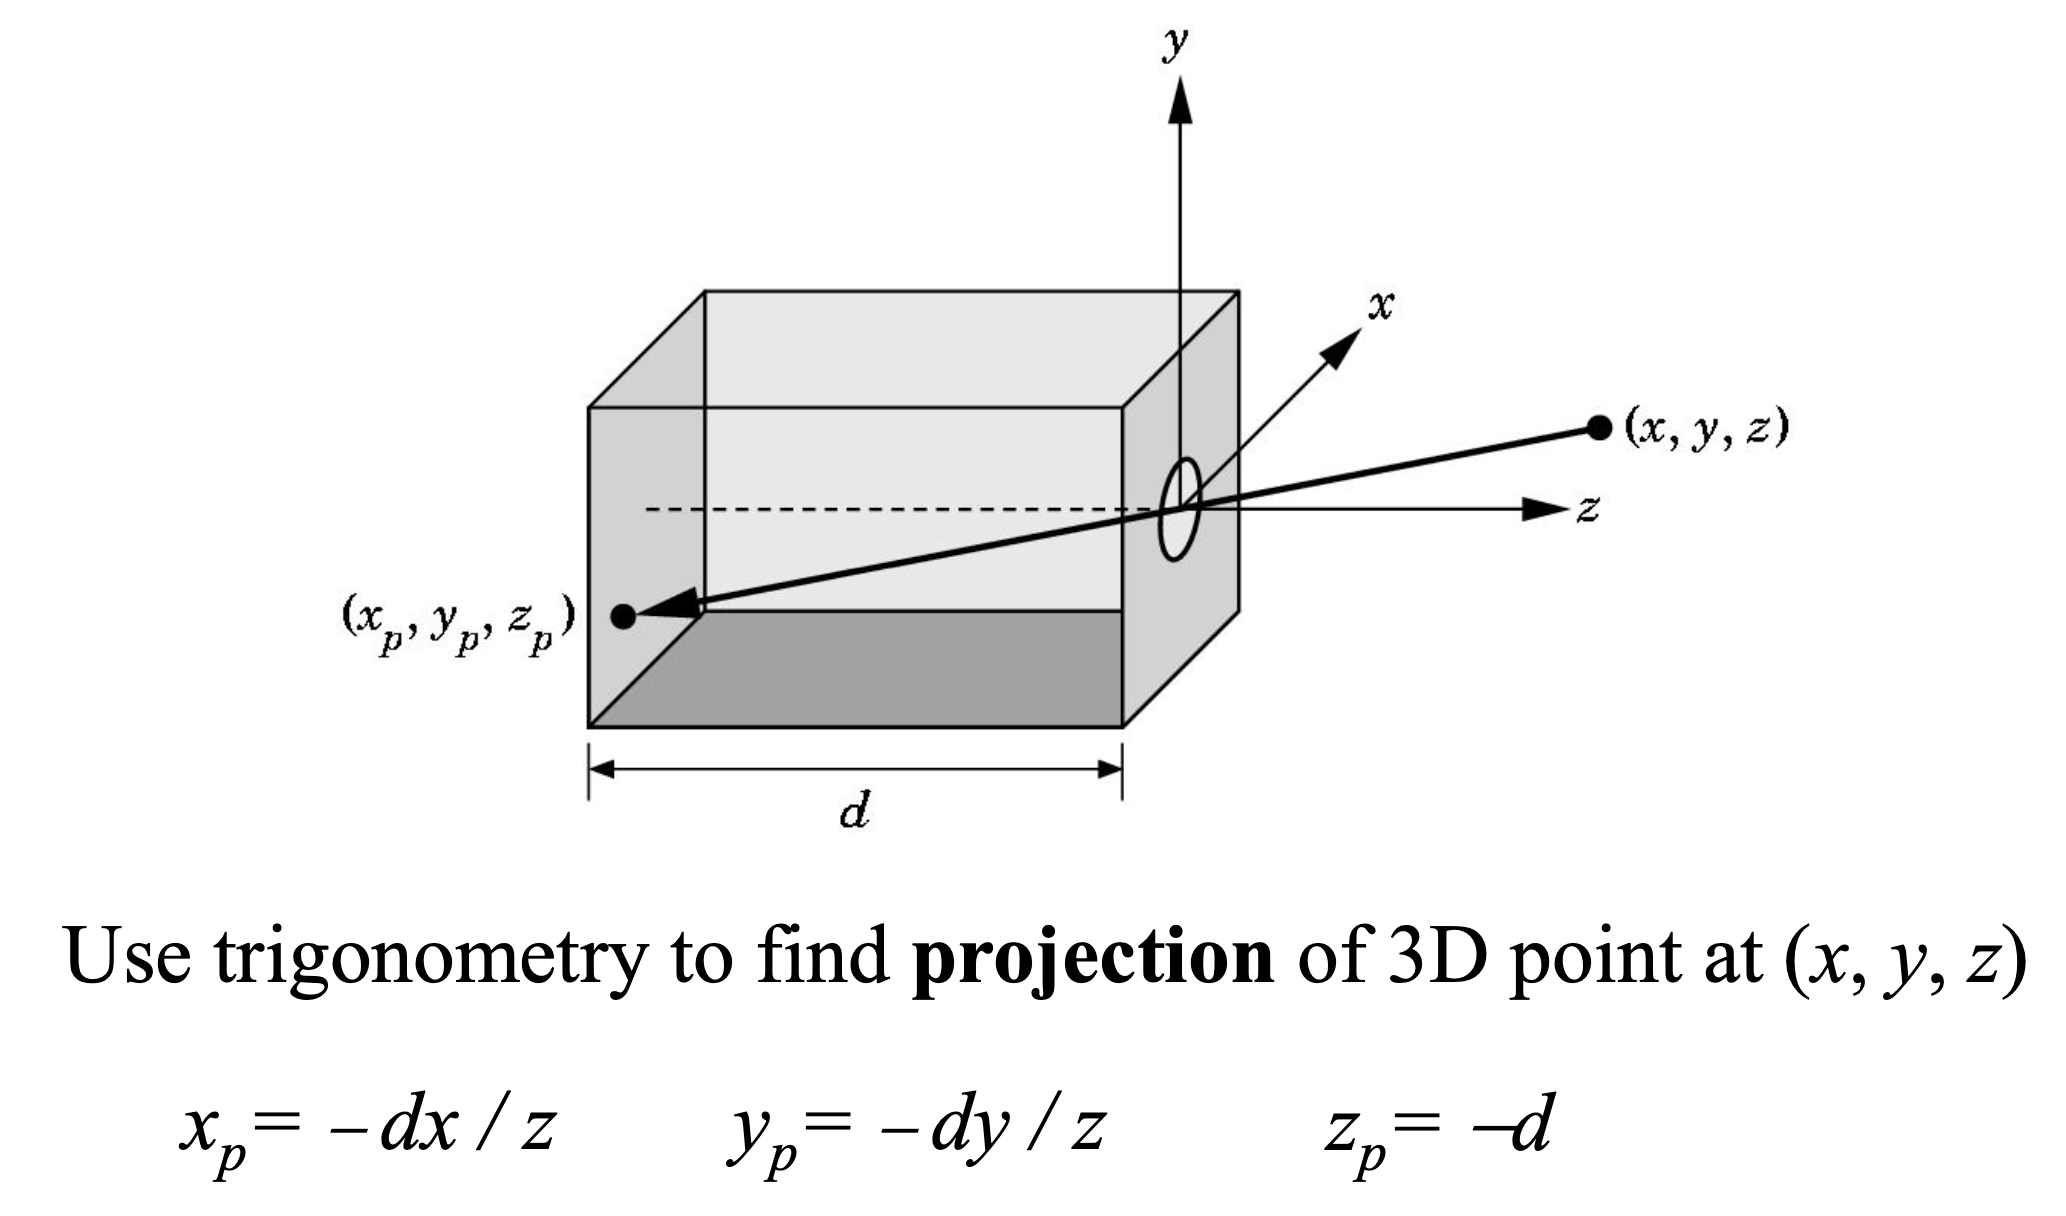
\includegraphics[width=\columnwidth]{L1/pinhole-camera}
    \paragraph{Synthetic camera model} \noindent \\
      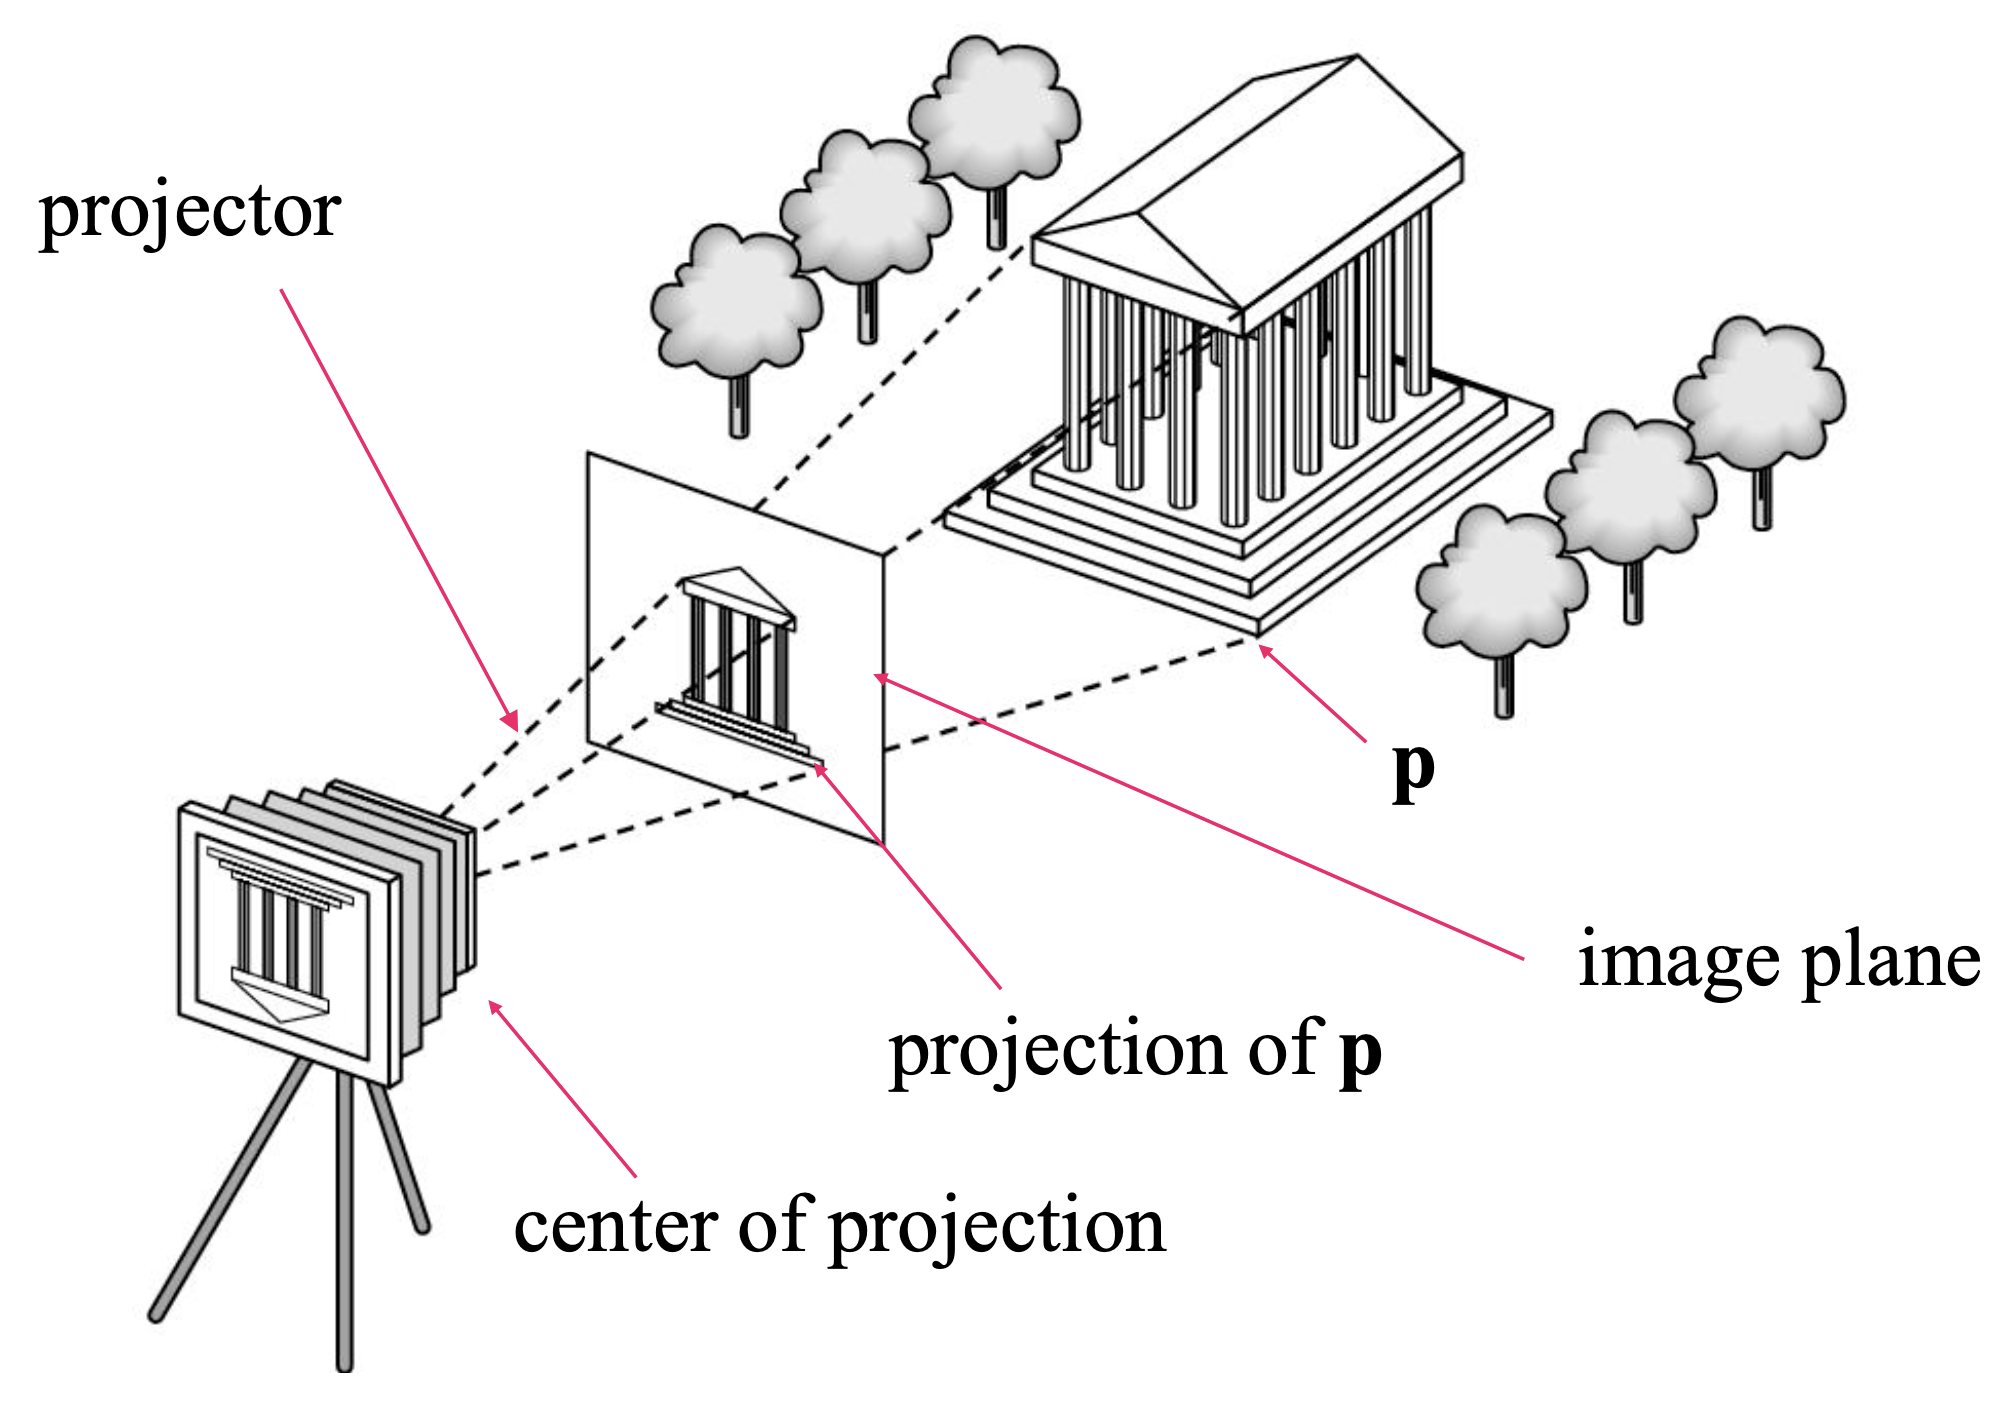
\includegraphics[width=\columnwidth]{L1/synthetic-camera-model}
  \subsection*{Luminance and color}
    \paragraph{Monochromatic images} Grayscale values stored
    \paragraph{Color images}
      \begin{hlist}
        \item Hue
        \item Saturation
        \item Lightness
      \end{hlist}
    \paragraph{Light}
      \begin{itemize}[leftmargin=*]
        \item Visible spectrum with wavelenght in range 350-750 nanometers
        \item Long wavelengths are red, short wavelengths are blue
      \end{itemize}
      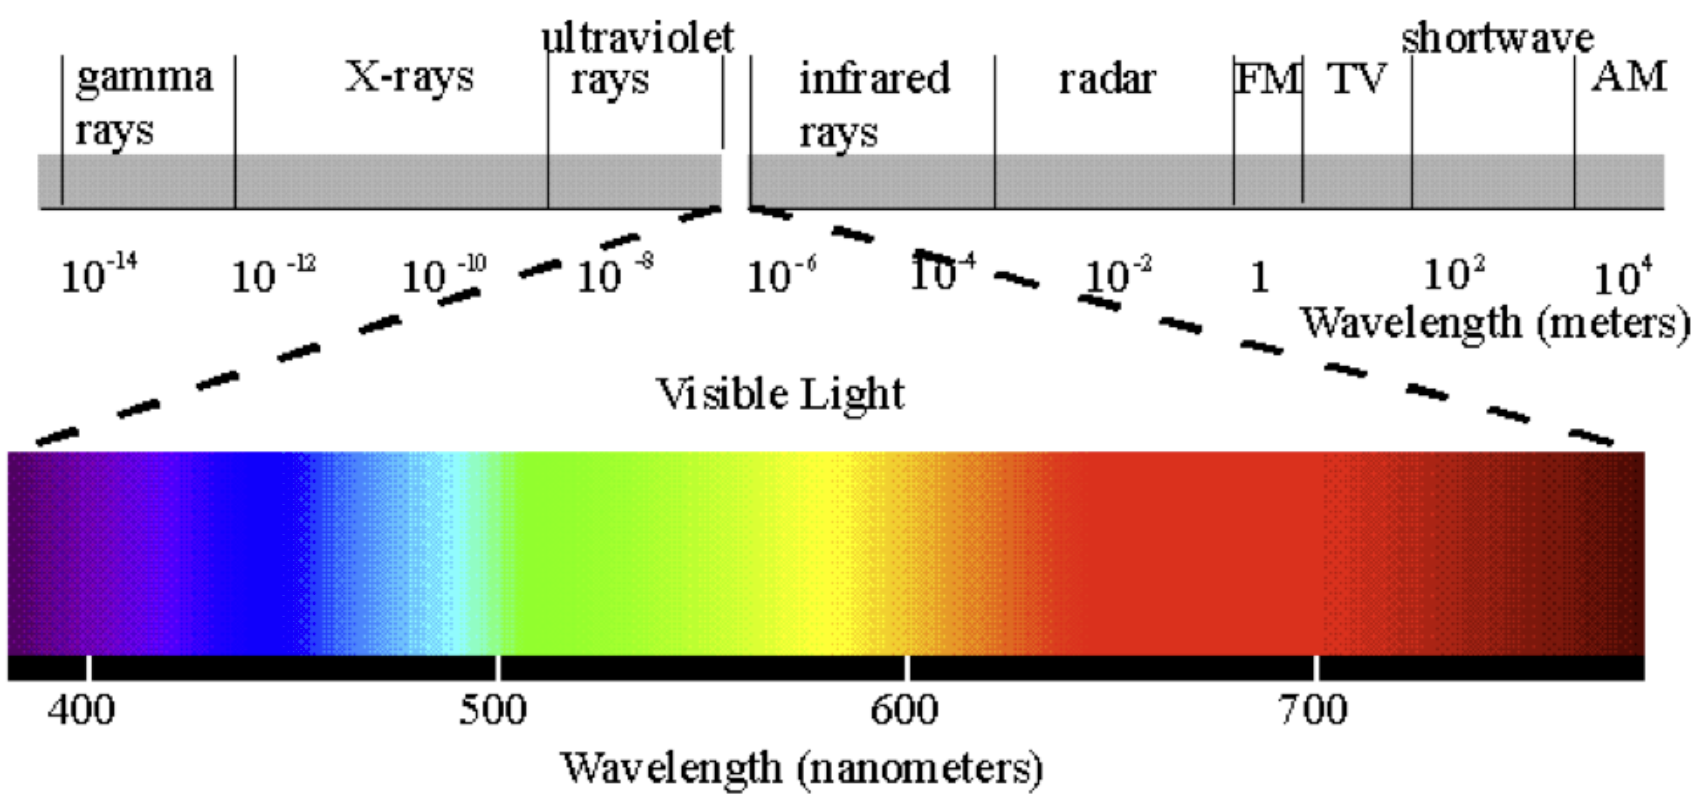
\includegraphics[width=\columnwidth]{L1/light}
  \subsection*{Three-color theory} \noindent
    Human visual system has two types of light sensors
    \begin{itemize}[leftmargin=*]
      \item Rods: good for monochromatic, night vision
      \item Cones: sensitive to color
    \end{itemize}
    \paragraph{Cones}
      \begin{itemize}[leftmargin=*]
        \item Three types of cones, sensitive to different wavelengths
        \item Use RGB to excite the cones
        \item Humans are more sensitive to green, then red, then blue. If there are only 8 bits total for RGB, allocate $3:3:2$ for R:G:B
      \end{itemize}
      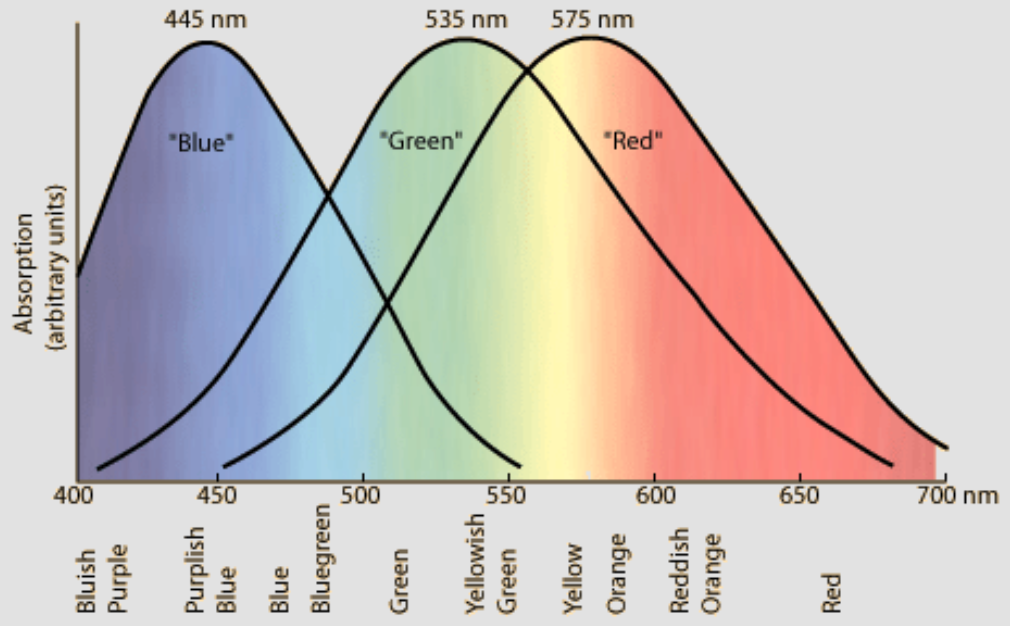
\includegraphics[width=\columnwidth]{L1/cones}
  \subsection*{Additive and subtractive color}
    \paragraph{Additive color} Add amounts of RGB
    \paragraph{Subtractive color}
      \begin{itemize}[leftmargin=*]
        \item Filter white light with cyan, magenta, and yellow filters
        \item Cyan = -Red; Magneta = -Green; Yellow = -Blue
      \end{itemize}
  \subsection*{Polygon rasterization}
    \begin{itemize}[leftmargin=*]
      \item Image is generated by processing a mesh of polygons
      \item Can be modelled as a pipeline
    \end{itemize}
    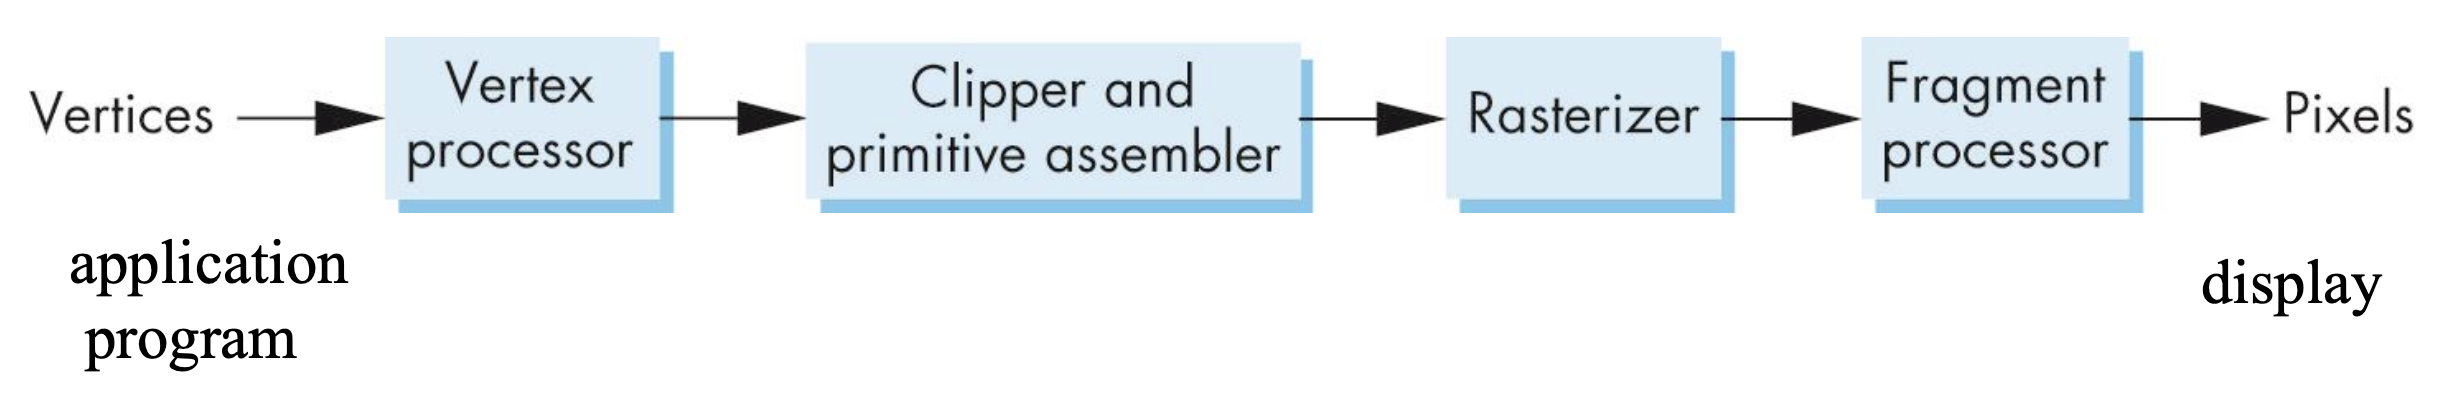
\includegraphics[width=\columnwidth]{L1/pipeline}
\section*{Elementary OpenGL}
  \subsection*{Function format} \noindent
    \ic{glVertex3f(x,y,z)}
    \begin{itemize}[leftmargin=*]
      \item \ic{gl} means it belongs to GL library
      \item \ic{Vertex} is the function name
      \item \ic{3} is the number of dimensions
      \item \ic{f} means the parameters are floats
    \end{itemize}
  \subsection*{Coordinate systems}
    \begin{itemize}[leftmargin=*]
      \item Units in \ic{glVertex} are determined by application; called object coords
      \item Camera is positioned in world coords
      \item Viewing specifications are specified in camera (eye) coords
      \item Internally, OpenGL converts vertices to camera (eye) coords, then to window coords
    \end{itemize}
  \subsection*{Camera} \noindent
    Defaults:
    \begin{itemize}[leftmargin=*]
      \item Placed at origin in world space
      \item Faces negative z direction
      \item Viewing volume is a box, centered at origin, with side length 2
    \end{itemize}
  \subsection*{OpenGL primitives} \noindent \\
    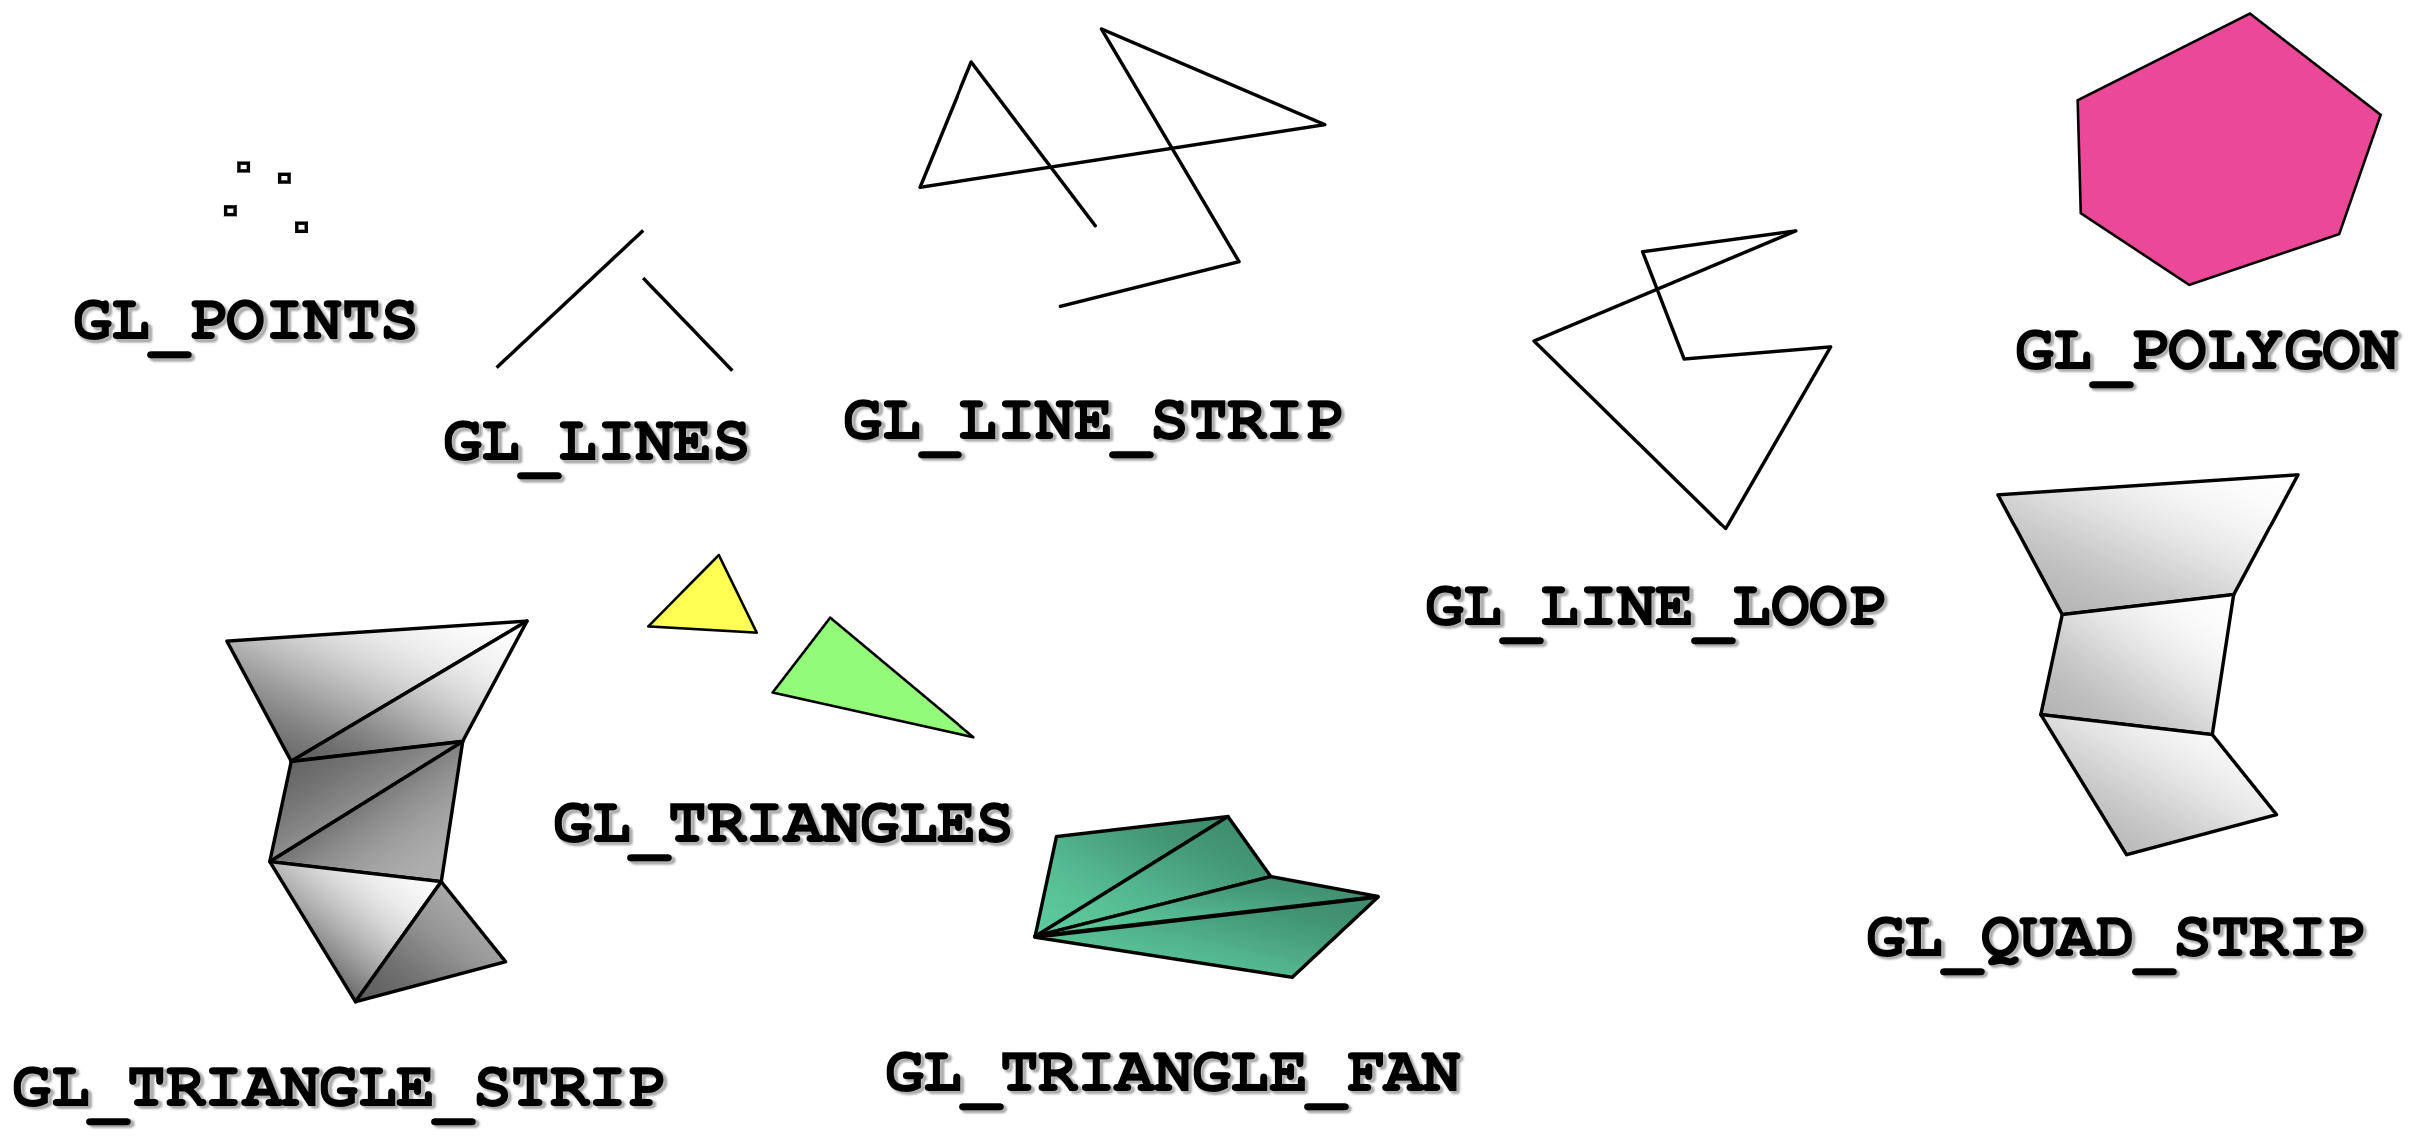
\includegraphics[width=\columnwidth]{L2/primitives}
    \begin{itemize}[leftmargin=*]
      \item Polygons are displayed correctly if they are
        \begin{itemize}[leftmargin=*]
          \item Simple: edges do not cross
          \item Convex: all points on line segment between any two points in the polygon or on the boundary are also in the polygon
          \item Flat: all vertices are in the same plane
        \end{itemize}
      \item If some condition is not true, OpenGL will still produce output, but it may not be what is desired
      \item Triangles satisfy all conditions
    \end{itemize}
    
\includegraphics[width=\columnwidth]{L2/polygons}
    \paragraph{Usage (right-angled triangle)}
      \begin{itemize}[leftmargin=*]
        \item Use \ic{glBegin} and \ic{glEnd} to mark the start/end of declaring vertices for a polygon
        \item Try to write in the display callback, so it is run once per display callback
      \end{itemize}
      \begin{minipage}{.6 \columnwidth}
        \begin{lstlisting}
glBegin(GL_TRIANGLES);
  glColor3f(1, 0, 0);
  glVertex3f(1, -1, 0);
  glVertex3f(-1, 1, 0);
  glVertex3f(-1, -1, 0);
glEnd();
        \end{lstlisting}
      \end{minipage}
      \hfill
      \begin{minipage}{.35 \columnwidth}
        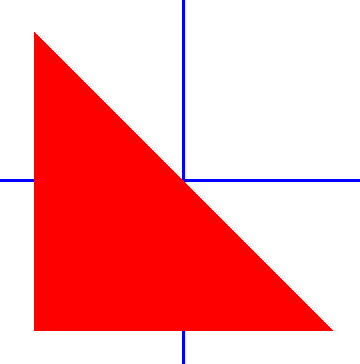
\includegraphics[width=\columnwidth]{L2/gl_triangles}  
      \end{minipage}
    \paragraph{Number of entities formed}
      Assume pass in $N$ vertices.
      \begin{center}
        \begin{tabular}{ |c|c| }
          \hline
          \textbf{Primitive} & \textbf{Result} \\ \hline
          \ic{GL_POINTS} & $N$ points \\ \hline
          \ic{GL_LINES} & $\frac{N}{2}$ lines \\ \hline
          \ic{GL_LINE_STRIP} & $N-1$ lines \\ \hline
          \ic{GL_LINE_LOOP} & $N$ lines \\ \hline
          \ic{GL_TRIANGLES} & $\frac{N}{3}$ triangles \\ \hline
          \ic{GL_TRIANGLE_STRIP} & $N-2$ triangles \\ \hline
          \ic{GL_TRIANGLE_FAN} & $N-2$ triangles \\ \hline
          \ic{GL_QUADS} & $\frac{N}{4}$ quads \\ \hline
          \ic{GL_QUAD_STRIP} & $\frac{N}{2} - 1$ quads \\ \hline
          \ic{GL_POLYGON} & 1 polygon \\ \hline
        \end{tabular}
      \end{center}
  \subsection*{Color}
    \begin{itemize}[leftmargin=*]
      \item Each color component/channel stored separately in frame buffer
      \item Usually 8 bits per component
      \item \ic{glColor3f} expects range from 0.0 to 1.0
      \item \ic{glColor3ub} expects range from 0 to 255
      \item Is part of OpenGL state, will be used until changed
    \end{itemize}
    \paragraph{Smooth color}
      \begin{itemize}[leftmargin=*]
        \item Default is smooth shading
          \begin{itemize}[leftmargin=*]
            \item Interpolates vertex colors across visible polygons
            \item \ic{glShadeModel(GL_SMOOTH)}
          \end{itemize}
        \item Alternative is flat shading
          \begin{itemize}[leftmargin=*]
            \item Color of first vertex determines fill color
            \item \ic{glShadeModel(GL_FLAT)}
          \end{itemize}
      \end{itemize}
  \subsection*{Viewport}
    \begin{itemize}[leftmargin=*]
      \item Specifies the drawing area within the window
      \item \ic{glViewport(x, y, width, height)}
      \item \ic{x, y} specify lower left corner of viewport rectangle
      \item Can have multiple, can overlap
      \item Use \ic{glClear(GL_COLOR_BUFFER_BIT)} to clear \textbf{entire window}
    \end{itemize}
\section*{Input and interaction} \noindent
  \subsection*{Input} \noindent
    \begin{itemize}[leftmargin=*]
      \item Devices contain a \textbf{trigger} that sends a signal to the OS
      \item When triggered,
        \begin{itemize}[leftmargin=*]
          \item Return info (\textbf{measure}) to the system
          \item Generate event, put into event queue
          \item The event queue starts after \ic{glutMainLoop()} is called in the \ic{main()} function
        \end{itemize}
      \item e.g. 
        \begin{hlist}
          \item Window (resize, expose, minimize)
          \item Mouse (click, motion)
          \item Keyboard (press, release)
          \item Idle (if no event)
        \end{hlist}
    \end{itemize}
  \subsection*{Callbacks} \noindent
    A callback is defined for each event
    \begin{itemize}[leftmargin=*]
      \item \ic{glutDisplayFunc} (required for GLUT programs)
        \begin{itemize}[leftmargin=*]
          \item \ic{void glutDisplayFunc(void (*func)(void))}
        \end{itemize}
      \item \ic{glutMouseFunc}
        \begin{itemize}[leftmargin=*]
          \item \ic{void glutMouseFunc(void (*func)(int button, int state, int x, int y))}
          \item \ic{button} is either left, middle, or right
          \item \ic{state} is either down or up
        \end{itemize}
      \item \ic{glutReshapeFunc} (window resizing)
        \begin{itemize}[leftmargin=*]
          \item \ic{void glutReshapeFunc(void (*func)(int width, int height))}
        \end{itemize}
      \item \ic{glutKeyboardFunc}
        \begin{itemize}[leftmargin=*]
          \item \ic{void glutKeyboardFunc(void (*func)(unsigned char key, int x, int y))}
          \item Returns ASCII code of depressed key and mouse location
        \end{itemize}
      \item \ic{glutIdleFunc} (useful for animations)
        \begin{itemize}[leftmargin=*]
          \item \ic{void glutIdleFunc(void (*func)(void))}
        \end{itemize}
      \item \ic{glutMotionFunc} (mouse moving while button is pressed)
        \begin{itemize}[leftmargin=*]
          \item \ic{void glutMotionFunc(void (*func)(int x, int y))}
        \end{itemize}
      \item \ic{glutPassiveMotionFunc} (mouse moving without button press)
        \begin{itemize}[leftmargin=*]
          \item \ic{void glutPassiveMotionFunc(void (*func)(int x, int y))}
        \end{itemize}
    \end{itemize}
    \subsubsection*{Display callback} \noindent
      \vspace{-0.5cm}
      \paragraph{Called when}
        \begin{itemize}[leftmargin=*]
          \item Window is 
            \begin{hlist}
              \item first opened
              \item reshaped
              \item uncovered
              \item restored from minimized state
            \end{hlist}
          \item User program wants to change the display
        \end{itemize}
      \paragraph{Posting redisplays} \noindent
        \begin{itemize}[leftmargin=*]
          \item Many events may invoke display callback function
          \item Hence, display callback may run multiple times in a single event loop pass
          \item Use \ic{glutPostRedisplay()} instead to set a flag that tells GLUT to execute the display call back function at the end of a single event loop
        \end{itemize}
    \subsubsection*{Reshape callback}
      \begin{itemize}[leftmargin=*]
        \item Good place to put viewing functions, since it is invoked when window is first opened
        \item Redisplay is posted automatically at the end of execution of the callback
      \end{itemize}
  \subsection*{Double buffering} \noindent
    \vspace{-0.5cm}
    \paragraph{Issue}
      \begin{itemize}[leftmargin=*]
        \item Drawing of info in frame buffer is decoupled from displaying the frame buffer
        \item We may see partially rendered frames on the display, that includes info from different frames (known as flickering)
      \end{itemize}
    \paragraph{Fix}
      \begin{itemize}[leftmargin=*]
        \item Maintain two buffers. Front buffer is displayed, while back buffer is written to
        \item Swap buffers at end of display callback (after writing is complete)
        \item Turn on: \ic{glutInitDisplayMode(... | GLUT_DOUBLE)}
        \item Swap buffers: \ic{glutSwapBuffers()}
      \end{itemize}
  \subsection*{Positioning}
    \begin{itemize}[leftmargin=*]
      \item OpenGL has origin at bottom left corner
      \item But for window system, mouse callback, motion callback, origin at top left corner
      \item Remember to invert $y$-coord when necessary
        \[ y_\text{opengl} = h - 1 - y_\text{win} \]
    \end{itemize}
  \subsection*{Reshaping a window} \noindent
    There are a few ways to redraw the scene. \\
    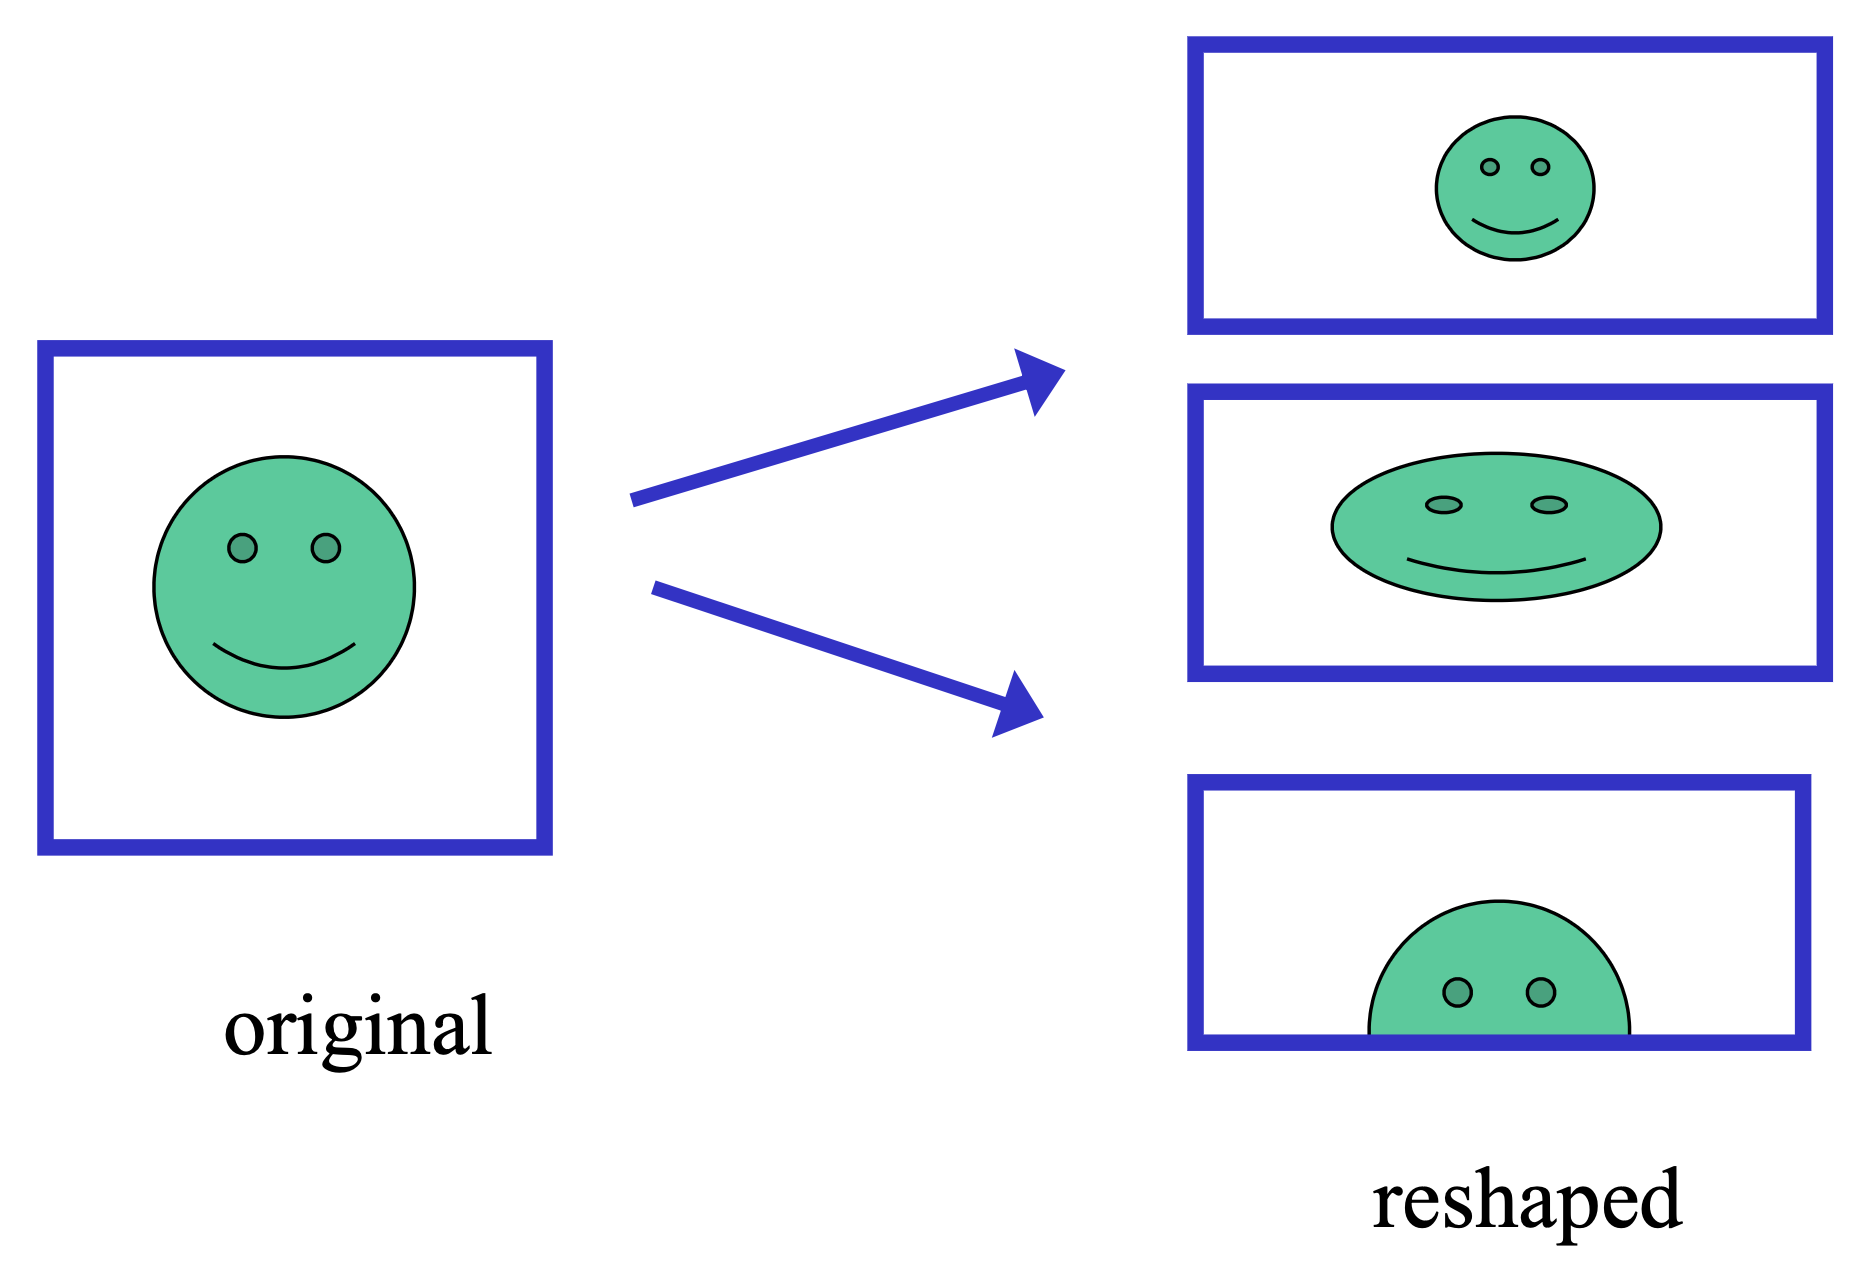
\includegraphics[width=0.6\columnwidth]{L3/reshape}
  \subsection*{Obtaining OpenGL state variables} \noindent
    Use \ic{void glGetIntegerv( GLenum pname, GLint *params )}
    \begin{itemize}[leftmargin=*]
      \item \ic{pname} is the state name
      \item \ic{params} is used to return the state variables
    \end{itemize}
  \subsection*{Special keys}
    \begin{itemize}[leftmargin=*]
      \item Special keys have constants defined in \ic{glut.h}:
        \begin{itemize}[leftmargin=*]
          \item Function key 1: \ic{GLUT_KEY_F1}
          \item Up arrow key: \ic{GLUT_KEY_UP}
        \end{itemize}
      \item Check if modifier keys are depressed
        \begin{itemize}[leftmargin=*]
          \item \ic{if(glutGetModifiers()} \\
                \ic{== GLUT_ACTIVE_CTRL)}
          \item Can emulate three-button mouse with one- or two-button mice
        \end{itemize}
    \end{itemize}
\section*{Geometry}
  \subsection*{Elements}
    \paragraph{Scalar} Fully described using magnitude
    \paragraph{Vector} Has direction and magnitude
    \paragraph{Vector space} Operations:
      \begin{itemize}[leftmargin=*]
        \item Scalar-vector multiplication
        \item Vector-vector addition
      \end{itemize}
    \paragraph{Point} Location in space
      \begin{itemize}[leftmargin=*]
        \item Point-point subtraction yields vector
      \end{itemize}
    \paragraph{Affine space} Point + vector space. Operations:
      \begin{itemize}[leftmargin=*]
        \item Scalar-vector multiplication
        \item Vector-vector addition
        \item Point-vector addition
        \item Scalar-scalar operations
        \item For a point $P$, define $1 \cdot P = P$, $0 \cdot P = \vec{0}$
      \end{itemize}
  \subsection*{Lines} \noindent
    For specific $P_0, d$, a line is the set of all points of the form
    \[ P(\alpha) = P_0 + \alpha d \]
    \paragraph{Representations}
      \begin{itemize}[leftmargin=*]
        \item Parametric form (using a point and a direction vector)
          \[ P(\alpha) = P_0 + \alpha d \]
        \item Paramteric form (using 2 points)
          \[ P(\alpha) = \alpha P_0 + (1 - \alpha) P_1 \]
        \item Explicit: $y = mx + h$
        \item Implicit: $ax + by + c = 0$
      \end{itemize}
    \paragraph{Ray}
      \begin{itemize}[leftmargin=*]
        \item Using the 1 point parametric definition of a line, a ray is a line with $\alpha \geq 0$.
          \[ P(\alpha) = P_0 + \alpha d \]
      \end{itemize}
    \paragraph{Line segment}
      \begin{itemize}[leftmargin=*]
        \item A line segment is bounded by 2 distinct points on a line.
        \item Using the 2 point parametric definition of a line, the line segment between $P_0$ and $P_1$ is a line with $0 \leq \alpha \leq 1$
          \[ P(\alpha) = \alpha P_0 + (1 - \alpha) P_1 \]
      \end{itemize}
  \subsection*{Planes} \noindent
    Defined either by
    \begin{itemize}[leftmargin=*]
      \item A point and two vectors, or
        \[ Plane(\alpha, \beta) = R + \alpha \vec{u} + \beta \vec{v} \]
      \item Three points
        \[ Plane(\alpha, \beta) = R + \alpha (Q-R) + \beta (P-Q) \]
      \item A point and a normal to the plane
        \[ (P-R) \cdot \vec{n} = 0 \]
        where $P$ is any point on the plane, and $\vec{n} = \vec{u} \times \vec{v}$.
    \end{itemize}
  \subsection*{Representation}
    \subsubsection*{Coordinate system (vector spaces)}
      \begin{itemize}[leftmargin=*]
        \item A basis $\{v_1, v_2, \cdots, v_n\}$ is a set of linearly independent vectors
        \item A vector can be expressed as $v = \alpha_1 v_1 + \alpha_2 v_2 + \cdots + \alpha_n v_n$
        \item The list of scalars $\{\alpha_1, \alpha_2, \cdots, \alpha_n\}$ is the representation of $v$ with respect to the given basis
        \item Can write the representation as a row or column vector
          \[ \vec{a} = \mat{\alpha_1 \alpha_2 \cdots, \alpha_n}^T = \mat{\alpha_1; \alpha_2; \vdots; \alpha_n} \]
      \end{itemize}
    \subsubsection*{Frames (affine spaces)}
      \begin{itemize}[leftmargin=*]
        \item Coordinate system is only able to specify vectors in 3D space
        \item Need a reference point to represent a point
        \item Frame is determined by tuple $(P_0, v_1, v_2, v_3)$
        \item Vector is still written as
          \begin{align*}
            v &= \alpha_1 v_1 + \alpha_2 v_2 + \alpha_3 v_3 \\
            =& \mat{v_1 v_2 v_3 P_0} \mat{\alpha_1 \alpha_2 \alpha_3 0}^T
          \end{align*}
        \item Point can now be written as
          \begin{align*}
            P &= P_0 + \beta_1 v_1 + \beta_2 v_2 + \beta_3 v_3 \\
            =& \mat{v_1 v_2 v_3 P_0} \mat{\beta_1 \beta_2 \beta_3 1}^T
          \end{align*}
      \end{itemize}
    \subsubsection*{Homogeneous coordinates} \noindent
      Given a coordinate vector $\mat{x y z w}^T$,
      \begin{itemize}[leftmargin=*]
        \item If $d = 0$ it is a vector
        \item Else it represents the point $\left(\frac{x}{w}, \frac{y}{w}, \frac{z}{w}\right)$.
      \end{itemize}
      \paragraph{Usefulness}
        \begin{itemize}[leftmargin=*]
          \item Standardized coordinate system that can represent both vectors and points simultaneously
          \item All standard transformation (rotaion, translation, scaling) can be implemented with 4 by 4 matrix multiplications
          \item Allows perspective projection (and perspective division) using matrix multiplication
        \end{itemize}
  \subsection*{Planar test for polygon in 3D space} \noindent
    Method 1:
    \begin{itemize}[leftmargin=*]
      \item Suppose polygon is defined by vertices $v_1, v_2, \cdots, v_n$
      \item Assume three consecutive vertices are not collinear
      \item Find normal vectors of triangle $v_1, v_2, v_3$, triangle $v_3, v_4, v_5$, and so on until triangle $v_{n-2}, v_{n-1}, v_n$
      \item Polygon is planar iff all the normal vectors are parallel
    \end{itemize}
    Method 2:
    \begin{itemize}[leftmargin=*]
      \item Suppose polygon is defined by vertices $v_1, v_2, \cdots, v_n$
      \item Assume three consecutive vertices are not collinear
      \item Form equation of plane using $v_1, v_2, v_3$
      \item Substitute in the rest of the points. Polygon is planar iff all the points agree with the equation
    \end{itemize}
  \subsection*{Convex test for polygon in $xy$ plane}
    \begin{itemize}[leftmargin=*]
      \item Suppose polygon is defined by vertices $v_1, v_2, \cdots, v_n$
      \item Assume three consecutive vertices are not collinear
      \item Compute normal vectors of triangle $v_1, v_2, v_3$, triangle $v_2, v_3, v_4$, and so on until triangle $v_n, v_1, v_2$
      \item Polygon is convex iff all normal vectors are in the same direction (not just parallel)
    \end{itemize}
\section*{Transformations}
  \subsection*{Affine transformations}
    \begin{itemize}[leftmargin=*]
      \item Preserves lines, so we can just transform endpoints of line segments and let implementation draw line segments
      \item Rigid body transformations: rotation, translation
      \item Scaling, shearing
    \end{itemize}
  \subsection*{Translation}
    \begin{itemize}[leftmargin=*]
      \item Move/translate/displace point to new location
      \item Displacement determined by vector $d$
    \end{itemize}
    \subsubsection*{Coordinate representation} \noindent
      Define
      \begin{align*}
        p &= \mat{x y z 1}^T \\
        p' &= \mat{x' y' z' 1}^T \\
        d &= \mat{d_x d_y d_z 0}^T
      \end{align*}
      Here, $p' = p + d$, so
      \begin{align*}
        x' &= x + d_x \\
        y' &= y + d_y \\
        z' &= z + d_z
      \end{align*}
    \subsubsection*{Matrix representation} \noindent
      We can also get $p' = Tp$ with the following matrix $T$:
      \[ T = T(d_x, d_y, d_z) = \mat{1 0 0 d_x; 0 1 0 d_y; 0 0 1 d_z; 0 0 0 1} \]
  \subsection*{Rotation (2D / about $z$-axis)} \noindent
    Consider \red{anti-clockwise} rotation about origin by $\theta$ degrees. \\
    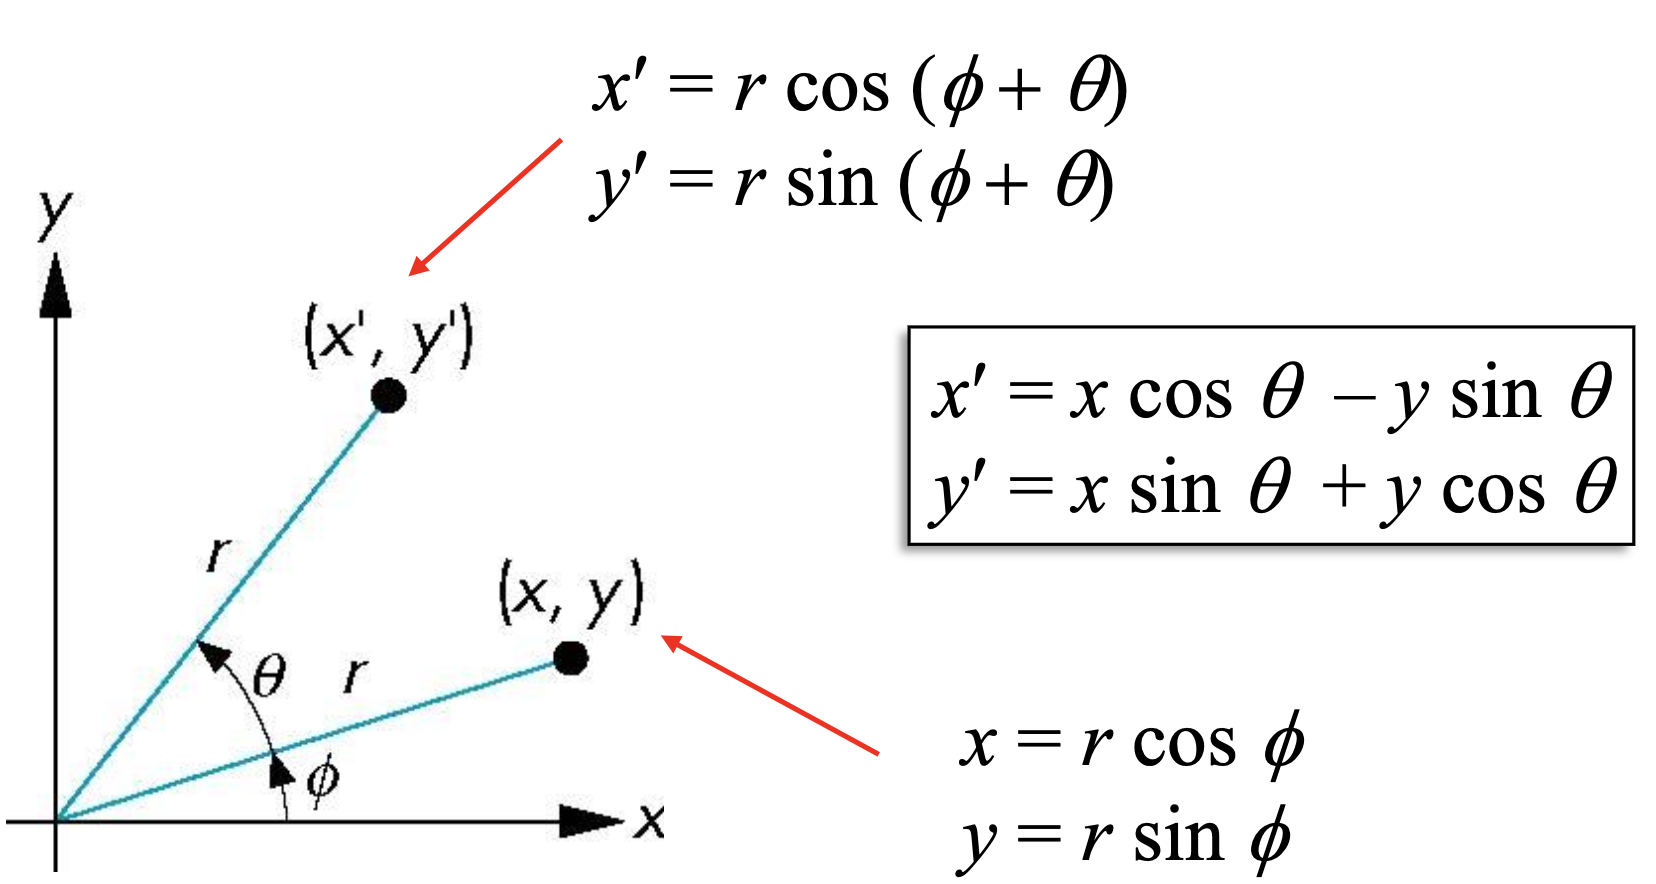
\includegraphics[width=\columnwidth]{L4/2d-rotation}
    Note that this is equivalent to rotation about $z$-axis, since $z$ is kept unchanged.
    \subsubsection*{Coordinate representation} \noindent
      \begin{align*}
        x' &= x \cos \theta - y \sin \theta \\
        y' &= x \sin \theta + y \cos \theta \\
        z' &= z
      \end{align*}
    \subsubsection*{Matrix representation} \noindent
      We have $p' = R_z(\theta) p$, where
      \[ R_z(\theta) = \mat{\cos\theta, -\sin\theta, 0 0; \sin\theta, \cos\theta, 0 0; 0 0 1 0; 0 0 0 1} \]
  \subsection*{Rotation about $x$ or $y$-axis} \noindent
    Similarly, for rotation about $x$ or $y$-axis, $x$ or $y$ is kept unchanged. Again, $\theta$ is measured anti-clockwise.
    \begin{align*}
      R_x(\theta) &= \mat{
        1 0 0 0;
        0 \cos\theta, -\sin\theta, 0;
        0 \sin\theta, \cos\theta, 0;
        0 0 0 1} \\
      R_y(\theta) &= \mat{
        \cos\theta, 0 \sin\theta, 0;
        0 1 0 0;
        -\sin\theta, 0 \cos\theta, 0;
        0 0 0 1}
    \end{align*}
    Note that rotations \red{do not commute}.
  \subsection*{Scaling}
    \subsubsection*{Coordinate representation} \noindent
      \begin{align*}
        x' &= s_x x \\
        y' &= s_y y \\
        z' &= s_z z
      \end{align*}
    \subsubsection*{Matrix representation} \noindent
      We have $p' = S(s_x, s_y, s_z) p$, where
      \[ S(s_x, s_y, s_z) = \mat{s_x 0 0 0; 0 s_y 0 0; 0 0 s_z 0; 0 0 0 1} \]
  \subsection*{Reflection} \noindent
    Corresponds to negative scale factors
    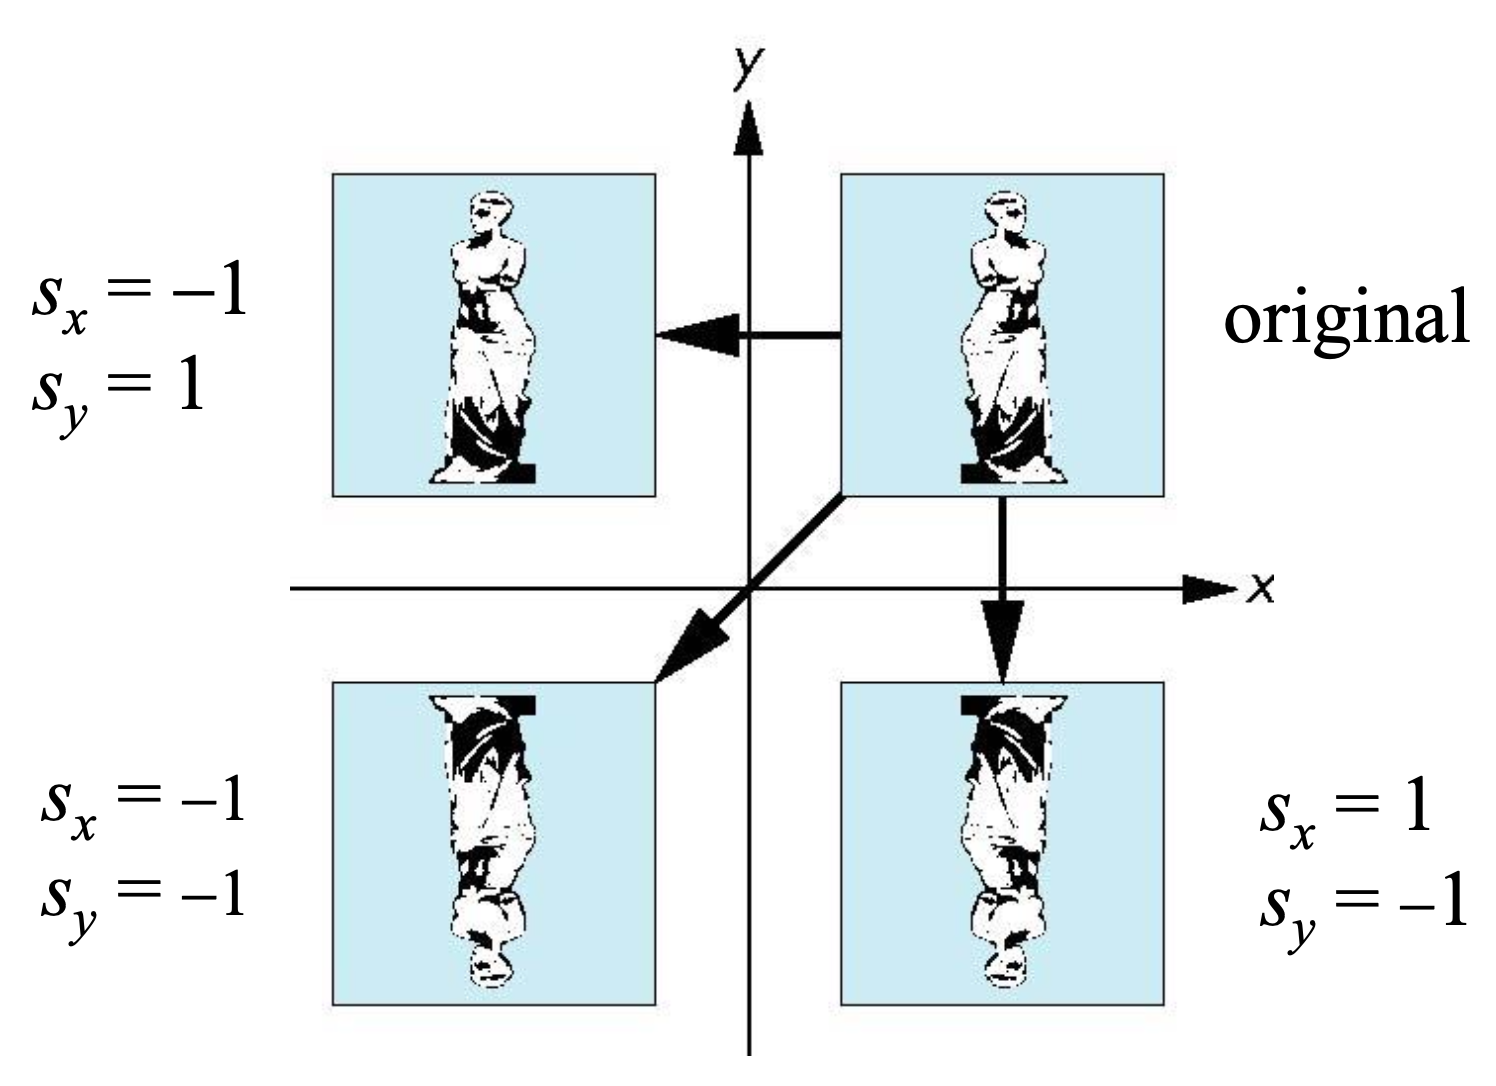
\includegraphics[width=\columnwidth]{L4/reflection}
  \subsection*{Concatenation} \noindent
    \begin{itemize}[leftmargin=*]
      \item We can form arbitrary affine transformation matrices by taking the product of the rotation, translation, scaling matrices
      \item $p' = DCBA(p)$ applies transformation A first, then B, C, D
      \item Note: 
        \[ (ABC)^T = C^T B^T A^T \]
    \end{itemize} 
  \subsection*{Inverses} \noindent
    Use geometric observations to get inverses:
    \begin{itemize}[leftmargin=*]
      \item Translation:
        \[ T^{-1} (d_x, d_y, d_z) = T(-d_x, -d_y, -d_z) \]
      \item Rotation: $R^{-1} (\theta) = R(-\theta) = R^T$
      \item Scaling:
        \[ S^{-1} (s_x, s_y, s_z) = S\left(\frac{1}{s_x}, \frac{1}{s_y}, \frac{1}{s_z}\right) \]
      \item Concatenation:
        \[ (ABC)^{-1} = C^{-1} B^{-1} A^{-1} \]
    \end{itemize}
  \subsection*{General rotation in 3D}
    \begin{enumerate}[leftmargin=*]
      \item Translate so that rotation axis passes through origin
      \item Rotate about the $x$-axis, so that the rotation axis lies in the $x-z$ plane
      \item Rotate about the $y$-axis, so that the rotation axis lies along the $z$-axis
      \item Perform the desired rotation by $\theta$, about the $z$-axis
      \item Apply inverse of step 3
      \item Apply inverse of step 2
      \item Apply inverse of step 1
    \end{enumerate}
  \subsection*{Instance transformation}
    \begin{itemize}[leftmargin=*]
      \item Draw object centered at origin, oriented with the axis, and at a standard size
      \item Scale, rotate, then translate
    \end{itemize}
  \subsection*{Shearing} \noindent
    Consider the following shear along the $x$-axis. \\
    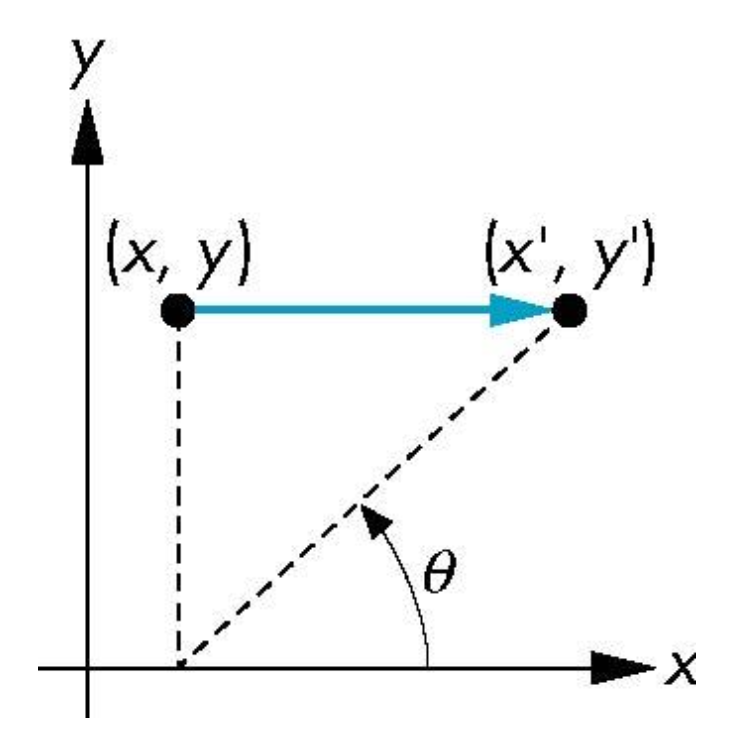
\includegraphics[width=0.6\columnwidth]{L4/shear}
    \subsubsection*{Coordinate representation} \noindent
      \begin{align*}
        x' &= x + y \cot \theta \\
        y' &= y \\
        z' &= z
      \end{align*}
    \subsubsection*{Matrix representation} \noindent
      We have $p' = H(\theta)p$, where
      \[ H(\theta) = \mat{1 \cot\theta, 0 0; 0 1 0 0; 0 0 1 0; 0 0 0 1} \]
  \subsection*{OpenGL transformations}
    \begin{itemize}[leftmargin=*]
      \item Model-View: \ic{glMatrixMode(GL_MODELVIEW)}
      \item Projection: \ic{glMatrixMode(GL_PROJECTION)}
    \end{itemize}
    \begin{center}
      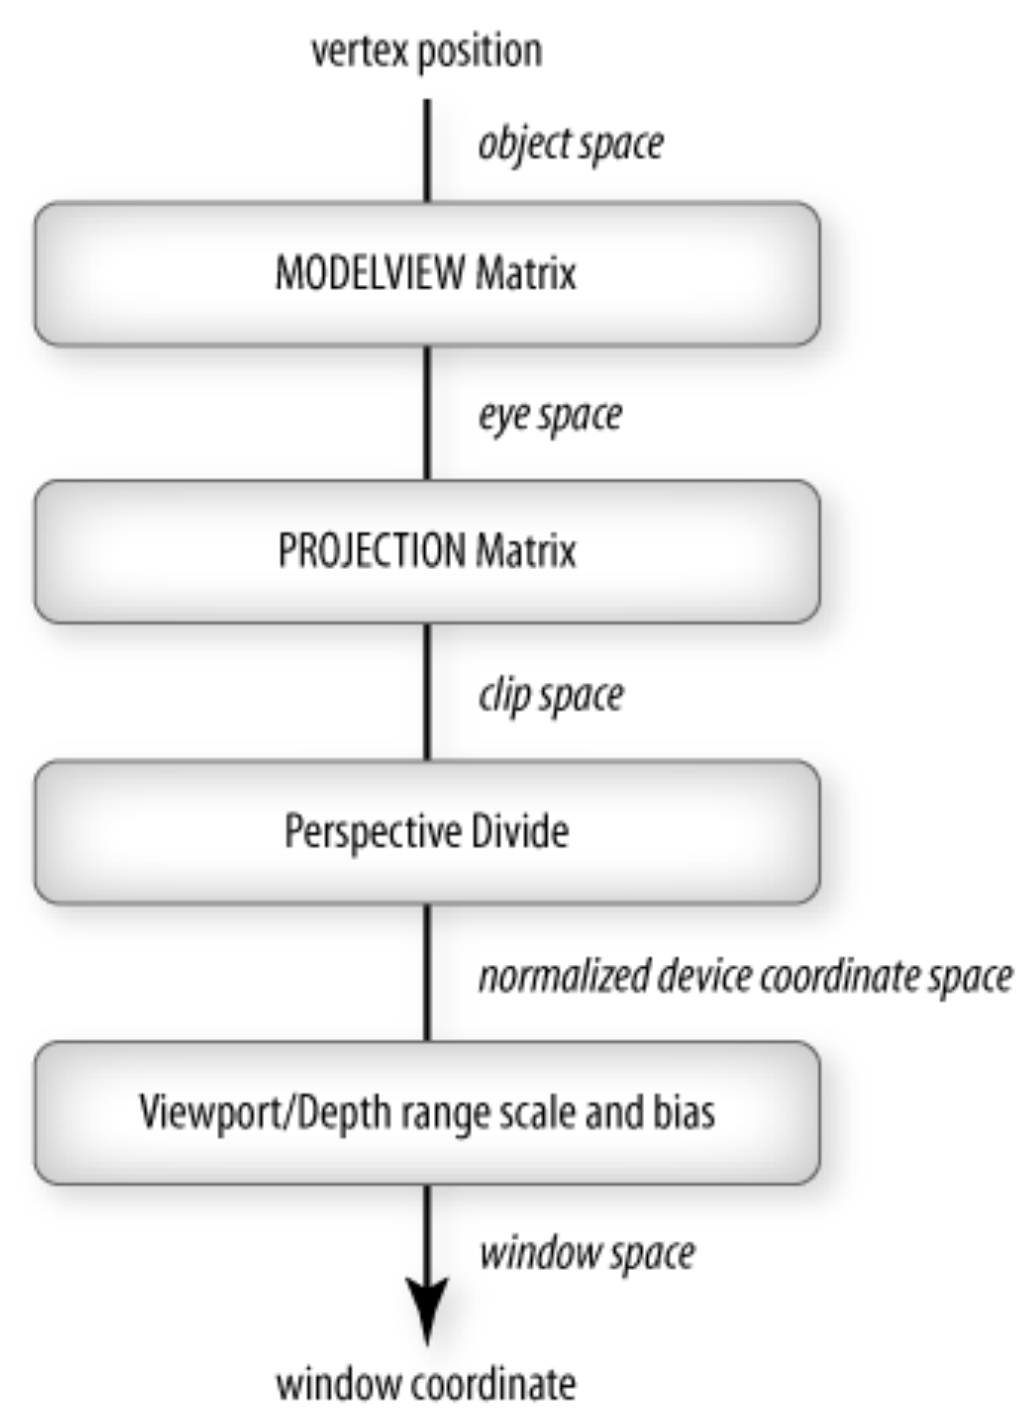
\includegraphics[width=0.6\columnwidth]{L4/opengl}
    \end{center}
    \subsubsection*{Current Transformation Matrix (CTM)}
      \begin{itemize}[leftmargin=*]
        \item Part of OpenGL state
        \item Can load/post-multiply matrices
        \item Since only post-multiply allowed, the last operation specified is actually the first transformation applied to vertices
        \begin{itemize}[leftmargin=*]
          \item When drawing a vertex, you pre-multiply the CTM to the point
          \item Hence the last operation is first applied
        \end{itemize}
        \item OpenGL stores has a different matrix for Model-View and Projection, which is loaded using \ic{glMatrixMode}
      \end{itemize}
    \subsubsection*{Model-View matrix}
      \begin{itemize}[leftmargin=*]
        \item (Modelling transformation) Transforms objects into the world space
        \item (View transformation) Positions the camera, aligning camera and world coordinate frames
        \item Projection matrix is used to defined view volume
      \end{itemize}
    \subsubsection*{Operations}
      \begin{itemize}[leftmargin=*]
        \item Load identity matrix: \ic{glLoadIdentity()}
        \item Rotation: \ic{glRotatef(theta, vx, vy, vz)}
          \begin{itemize}[leftmargin=*]
            \item \ic{theta} is in degrees
            \item \ic{(vx, vy, vz)} is axis of rotation
            \item Convert radian to degrees by multiplying by $\frac{180}{\pi}$
          \end{itemize}
        \item Translation: \ic{glTranslatef(dx, dy, dz)}
        \item Scale: \ic{glScalef(sx, sy, sz)}
        \item Each has \ic{(f)loat} and \ic{(d)ouble} format
      \end{itemize}
      \paragraph{Arbitrary matrices}
        \begin{itemize}[leftmargin=*]
          \item Load arbitrary matrix: \ic{glLoadMatrixf(m)}
          \item Post-multiply by arbitrary matrix: \ic{glMultMatrixf(m)}
        \end{itemize}
      \paragraph{Matrix stacks}
        \begin{itemize}[leftmargin=*]
          \item Might want to save transformation matrices for later use
          \item OpenGL maintains a stack for each matrix mode
          \item \ic{glPushMatrix()} pushes a copy of the top of the stack onto it
          \item \ic{glPopMatrix()} pops the stack
        \end{itemize}
\columnbreak
\section*{Camera \& Viewing}
  \subsection*{Planar geometric projections}
    \begin{itemize}[leftmargin=*]
      \item Project onto a plane
      \item Preserves lines, so we can just transform endpoints of line segments and let implementation draw line segments
      \item May not preserve angles
      \item Non-planar projection surfaces needed for applications such as map construction
    \end{itemize}
    \paragraph{Examples} Perspective projection, parallel projection
    \paragraph{Projectors} are lines that either
      \begin{itemize}[leftmargin=*]
        \item Converge at center of projection
        \item Are parallel
      \end{itemize}
    \subsubsection*{Orthographic projection}
      \begin{itemize}[leftmargin=*]
        \item Special case of parallel projection, where projectors are orthogonal to projection surface
        \item In the default orthographic view, points are projected along the $z$-axis, onto the plane $z=0$
      \end{itemize}
    \subsubsection*{Perspective projection}
      \begin{itemize}[leftmargin=*]
        \item Projectors converge at center of projection
        \item Objects further from viewer are projected smaller (dimunition)
        \item Equal distances along a line are not projected into equal distances (non-uniform foreshortening)
        \item Angles preserved only in planes which are parallel to the projection plane
      \end{itemize}
    \subsubsection*{Projection matrix}
      \begin{itemize}[leftmargin=*]
        \item Basically selects a lens
        \item Sets view volume/clipping volume, defining the region of the 3D world that appears in the viewport
      \end{itemize}
  \subsection*{Spaces} \noindent
    \begin{itemize}[leftmargin=*]
      \item Refer to slides.
      \item Note that world space is after the model transformation, but since OpenGL combines the model and view transformations into a single matrix, this space is not explicitly in the pipeline
    \end{itemize}
  \subsection*{Model transformation}
    \begin{itemize}[leftmargin=*]
      \item Prior to this, objects are typically at the origin, possibly at unit size
      \item This transformation uses rotation, scaling, translation to put the object in its intended position in the world
    \end{itemize}
  \subsection*{\ic{gluLookAt()} / View transformation}
    \subsubsection*{Usage}
      \begin{itemize}[leftmargin=*]
        \item \ic{gluLookAt(eyeX, eyeY, eyeZ, atX, atY, atZ, upX, upY, upZ)}
        \item \ic{(eyeX, eyeY, eyeZ)} specifies the position of the camera
        \item \ic{(atX, atY, atZ)} specifies the point that the camera should look at
        \item up-vector is the vector from the eye position to \ic{(upX, upY, upZ)}.
        \item Note that camera should face negative $z$ direction
      \end{itemize}
    \subsubsection*{up-vector}
      \begin{itemize}[leftmargin=*]
        \item Lies anywhere on the original $y-z$ plane, but should not lie on $z$-axis (view direction)
        \item Does not need to be perpendicular to view direction (negative z direction)
        \item Cross product of up-vector and view direction gives unique $x$-axis
        \item Cross product of $x$-axis and view direction gives unique $y$-axis
        \item Cross product of $x$-axis and $y$-axis gives unique $z$-axis
      \end{itemize}
      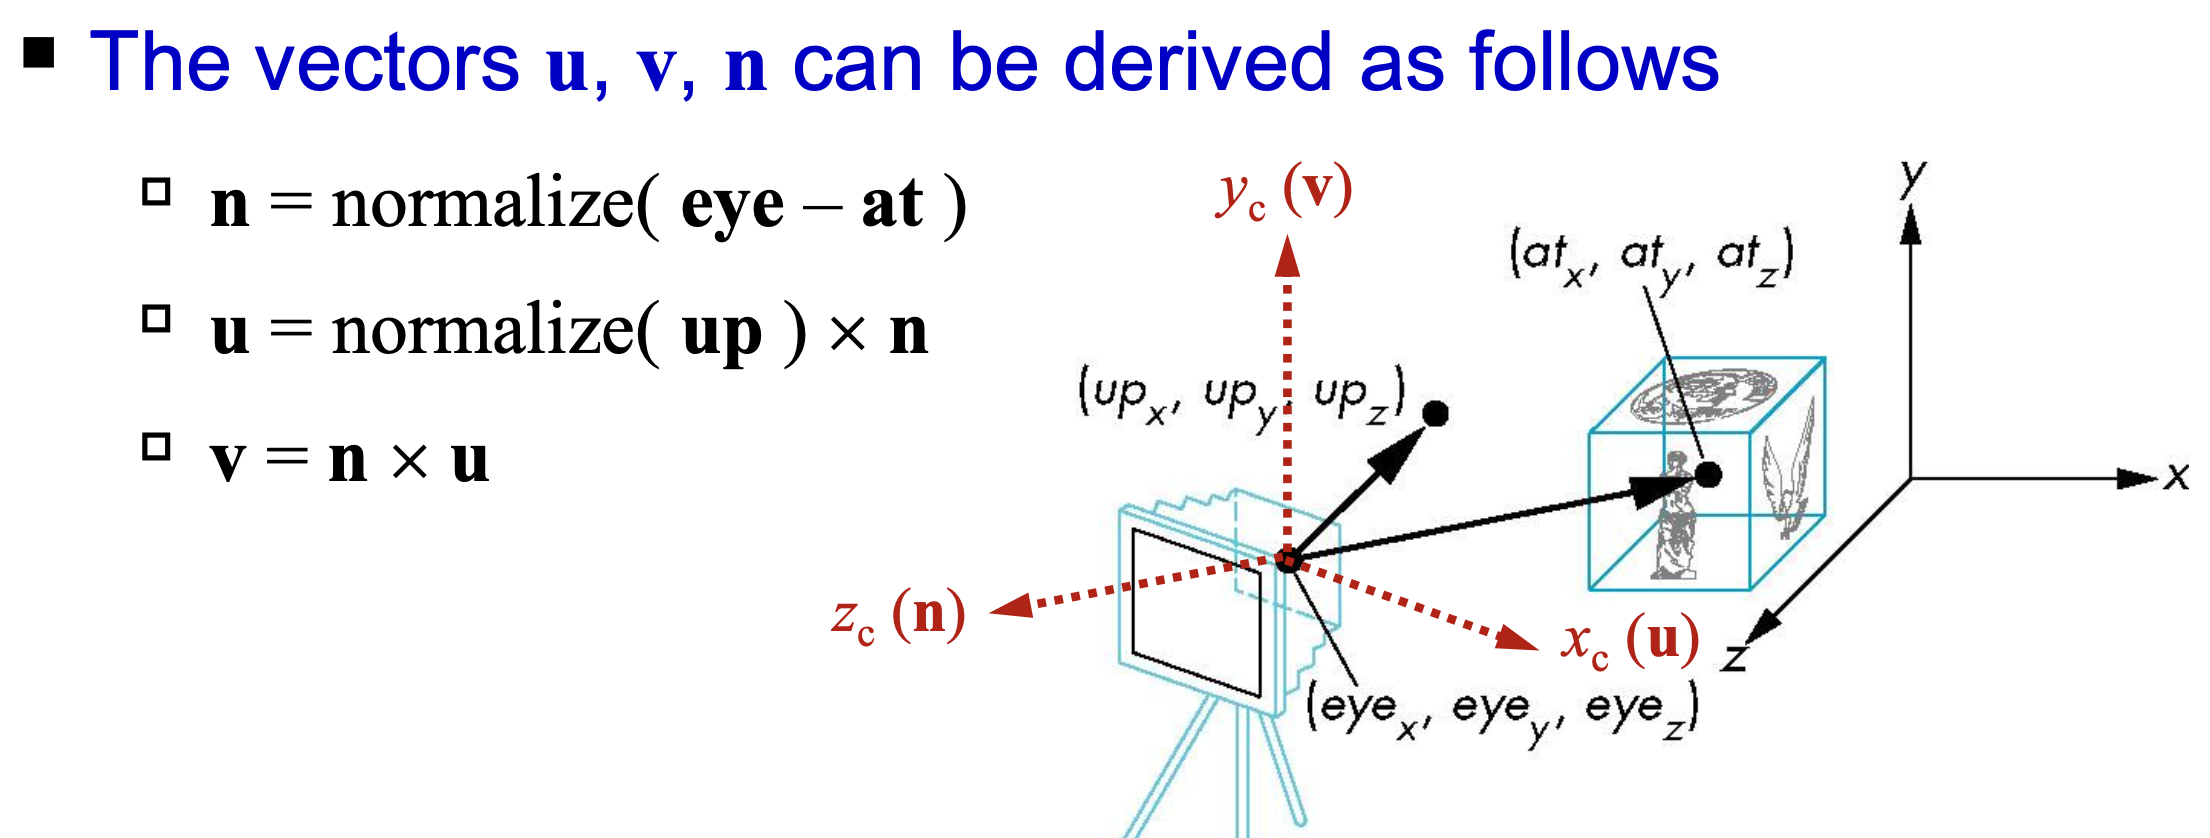
\includegraphics[width=\columnwidth]{L5/gluLookAt}
    \subsubsection*{Concept}
      \begin{itemize}[leftmargin=*]
        \item Positions camera at required location and orientation wrt world frame
        \item Internally generates transformation matrix that can be used to express all points in world frame wrt camera frame (i.e. view transformation)
      \end{itemize}
      \begin{flalign*}
        & M_{view} = RT & \\
        &= \mat{u_x u_y u_z 0; v_x v_y v_z 0; n_x n_y n_z 0; 0 0 0 1} \mat{1 0 0 -e_x; 0 1 0 -e_y; 0 0 1 -e_z; 0 0 0 1}
      \end{flalign*}
      \begin{itemize}[leftmargin=*]
        \item Translation $T$ moves camera to origin
        \item Rotation $R$ aligns camera frame axes to world frame axes
        \item $u,v,n$ defined in picture above
        \item $e$ is the eye position
      \end{itemize}
    \subsubsection*{Transformation of normal vectors} \noindent
      Let a plane equation be given by $n \cdot v = 0$. Let $M_t$ be the upper-left 3 by 3 submatrix of the model-view transformation matrix $M$.
      \begin{align*}
        n \cdot v &= 0 \\
        n^T v &= 0 \\
        n^T M_t^{-1} M_t v &= 0
      \end{align*}
      But notice that $M_t v$ produces a vector in eye coordinates. Now we have
      \[ n^T M_t^{-1} \cdot v_{eye} = 0 \]
      which is the equation of a plane, which was transformed by $M_t$. Hence, the new normal is $n^T M_t^{-1}$. This is a row vector pre-multiplied to a matrix, which gives a row vector. To get a column vector, transpose this, getting $(M_t^{-1})^T n$.
      \paragraph{Result}
        \begin{itemize}[leftmargin=*]
          \item Normal vectors are pre-multiplied by $(M_t^{-1})^T$, where $M_t$ is the upper-left 3 by 3 submatrix of $M$.
          \item If $M_t$ is a rotation, then $M_n = M_t$, since $(M_t)^{-1} = (M_t)^T$.
        \end{itemize}
  \subsection*{Projection matrix}
    \subsubsection*{Projections}
      \begin{itemize}[leftmargin=*]
        \item Specifies view volume for projection wrt camera frame
        \item 3D region of scene to appear in the rendered image
      \end{itemize}
\end{multicols*}
\begin{multicols*}{2}
    \subsubsection*{Matrix}
      \begin{itemize}[leftmargin=*]
        \item Maps points in view volume to canonical view volume
        \item Canonical view volume is the 2 by 2 by 2 cube bounded by the planes $x = \pm 1, y = \pm 1, z = \pm 1$, also called Normalized Device Coordinates
        \item Preserves depth order (in $z$-coordinate)
        \item Preserves lines
        \item This intermediate canonical view volume is then mapped to the viewport
      \end{itemize}
  \subsection*{Orthographic projection} \noindent
    Example code:
    \begin{lstlisting}
// Set the matrix mode
glMatrixMode(GL_PROJECTION); 
// Reset the matrix and apply default
// view volume
glLoadIdentity();
glOrtho(-1.0, 1.0, -1.0, 1.0, -1.0, 1.0);
    \end{lstlisting}
    \subsubsection*{\ic{glOrtho}}
      \begin{itemize}[leftmargin=*]
        \item \ic{glOrtho(left, right, bottom, top, near, far)}
        \item \ic{left, right, bottom, top} specify coords of clipping planes
        \item \ic{near} and \ic{far} specify displacements from $z=0$ to near/far clipping planes in the -ve $z$-direction. Since the camera faces the -ve $z$ direction, a -ve number means that the plane is behind the camera.
        \item \ic{gluOrtho2D(left, right, bottom, top)} is equivalent to \ic{glOrtho(left, right, bottom, top, -1, 1)}
        \item Transformation matrix
          \begin{flalign*}
            & \mat{\dfrac{2}{right-left}, 0 0 \dfrac{-(right+left)}{right - left};
              0 \dfrac{2}{top-btm}, 0 \dfrac{-(top+btm)}{top - btm};
              0 0 \dfrac{-2}{far-near} \dfrac{-(far+near)}{far - near};
              0 0 0 1} & \\
                       &= S\left(\frac{2}{right-left}, \frac{2}{top-btm}, \frac{2}{near-far}\right) \cdot \\
                       & T\left(\frac{-(right+left)}{2}, \frac{-(top+btm)}{2}, \frac{far+near}{2}\right)
          \end{flalign*}
        \item Note that $z = -near$ is mapped to $z = -1$, and $z = -far$ to $z = 1$
      \end{itemize}
    \subsubsection*{Viewport transformation}
      \begin{itemize}[leftmargin=*]
        \item Canonical view volume is mapped to the viewport (from NDC to window coords). Consider viewport of size $(w, h)$ and bottom left corner $(x_{vp}, y_{vp})$.
          \begin{flalign*}
            & \frac{x_{NDC} - (-1)}{2} = \frac{x_{win} - x_{vp}}{w} \Rightarrow x_{win} = x_{vp} + \frac{w(x_{NDC} + 1)}{2} & \\
            & \frac{y_{NDC} - (-1)}{2} = \frac{y_{win} - y_{vp}}{h} \Rightarrow y_{win} = y_{vp} + \frac{h(y_{NDC} + 1)}{2} \\
            & z_{win} = \frac{z_{NDC} + 1}{2}
          \end{flalign*}
        \item By default, $0 \leq z_{win} \leq 1$, for $z$-buffer hidden surface removal
      \end{itemize}
  \subsection*{Perspective projection} \noindent
    \vspace{-.5cm}
    \subsubsection*{Example}
      \begin{itemize}[leftmargin=*]
        \item Center of projection at origin
        \item Projection plane is $z=d$ where $d < 0$
      \end{itemize}
      \paragraph{Coordinates}
        \begin{center}
          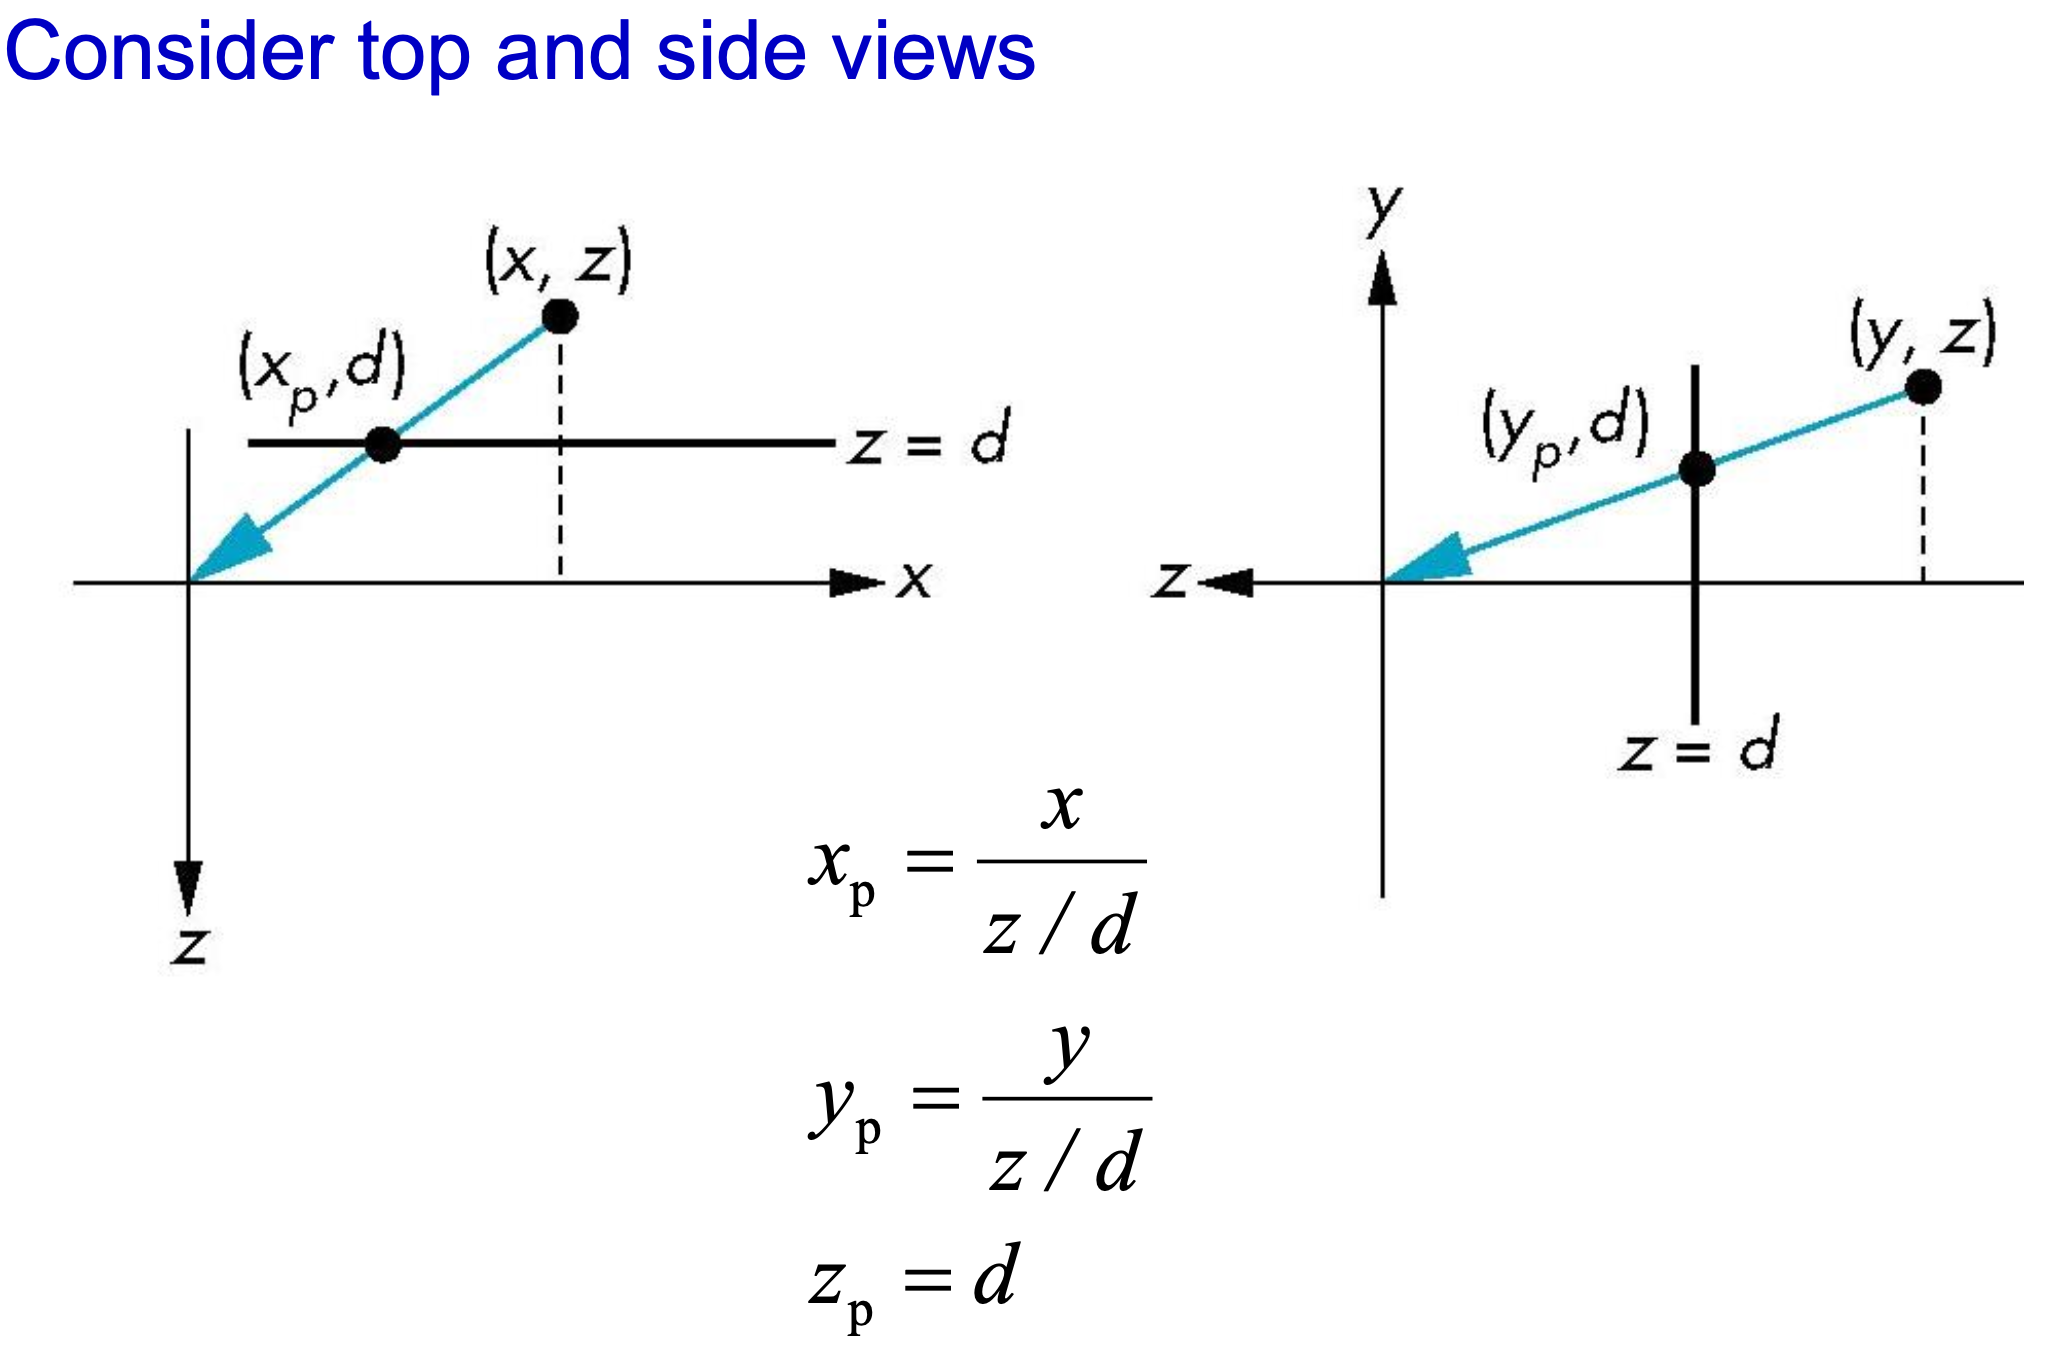
\includegraphics[width=0.6\columnwidth]{L5/perspective}
        \end{center}
      \paragraph{Matrix}
        We have $p = Mq$, where
        \[
          p = \mat{x;y;z;z/d} \quad
          M = \mat{1 0 0 0; 0 1 0 0; 0 0 1 0; 0 0 1/d 0} \quad
          q = \mat{x;y;z;1}
        \]
      \paragraph{Perspective division}
        \begin{itemize}[leftmargin=*]
          \item Notice that in the transformed point $p$, $z/d \neq 1$, so we divide by $z/d$ to return from homogeneous coordinates
          \item This is called perspective division
            \[
              p = \mat{x;y;z;z/d}
              \xrightarrow{
                \begin{subarray}
                  \text{perspective} \\
                  \text{division}
                \end{subarray}
              }
              p' = \mat{\frac{x}{z/d}; \frac{y}{z/d}; d; 1}
            \]
        \end{itemize}
    \subsubsection*{\ic{glFrustum()}}
      \begin{itemize}[leftmargin=*]
        \item \ic{glFrustum(left, right, bottom, top, near, far)}
        \item Maps the view frustum to canonical view volume, which will then be mapped to viewport
        \item Matrix
          \[\mat{
            \dfrac{2 \cdot near}{right - left} 0 \dfrac{right+left}{right-left} 0;
            0 \dfrac{2 \cdot near}{top-btm} \dfrac{top+btm}{top-btm} 0;
            0 0 \dfrac{-(far+near)}{far-near} \dfrac{-2 \cdot far \cdot near}{far - near};
            0 0 -1 0
          }\]
      \end{itemize}
    \subsubsection*{\ic{gluPerspective()}}
      \begin{itemize}[leftmargin=*]
        \item \ic{glFrustum} allows for off-center, non-symmetric view volume
        \item But we often want a symmetric view volume. We can use \\
          \ic{gluPerspective(fovy, aspect, near, far)} instead
          \begin{itemize}[leftmargin=*]
            \item \ic{fovy} specifies the fov angle in degrees in the $y$-direction
            \item \ic{aspect} is $\dfrac{width}{height}$
            \item \ic{near} and \ic{far} specify distances to near/far planes
          \end{itemize}
        \item Let $f = \cot\left(\dfrac{fovy}{2}\right)$. The matrix is
          \[ \mat{
            \dfrac{f}{aspect} 0 0 0; 0 f 0 0; 0 0 \dfrac{far+near}{near - far} \dfrac{2 \cdot far \cdot near}{near - far}; 0 0 -1 0
          }\]
      \end{itemize}
\section*{OpenGL rendering pipeline} \noindent
  \vspace{-0.5cm}
  \begin{center}
    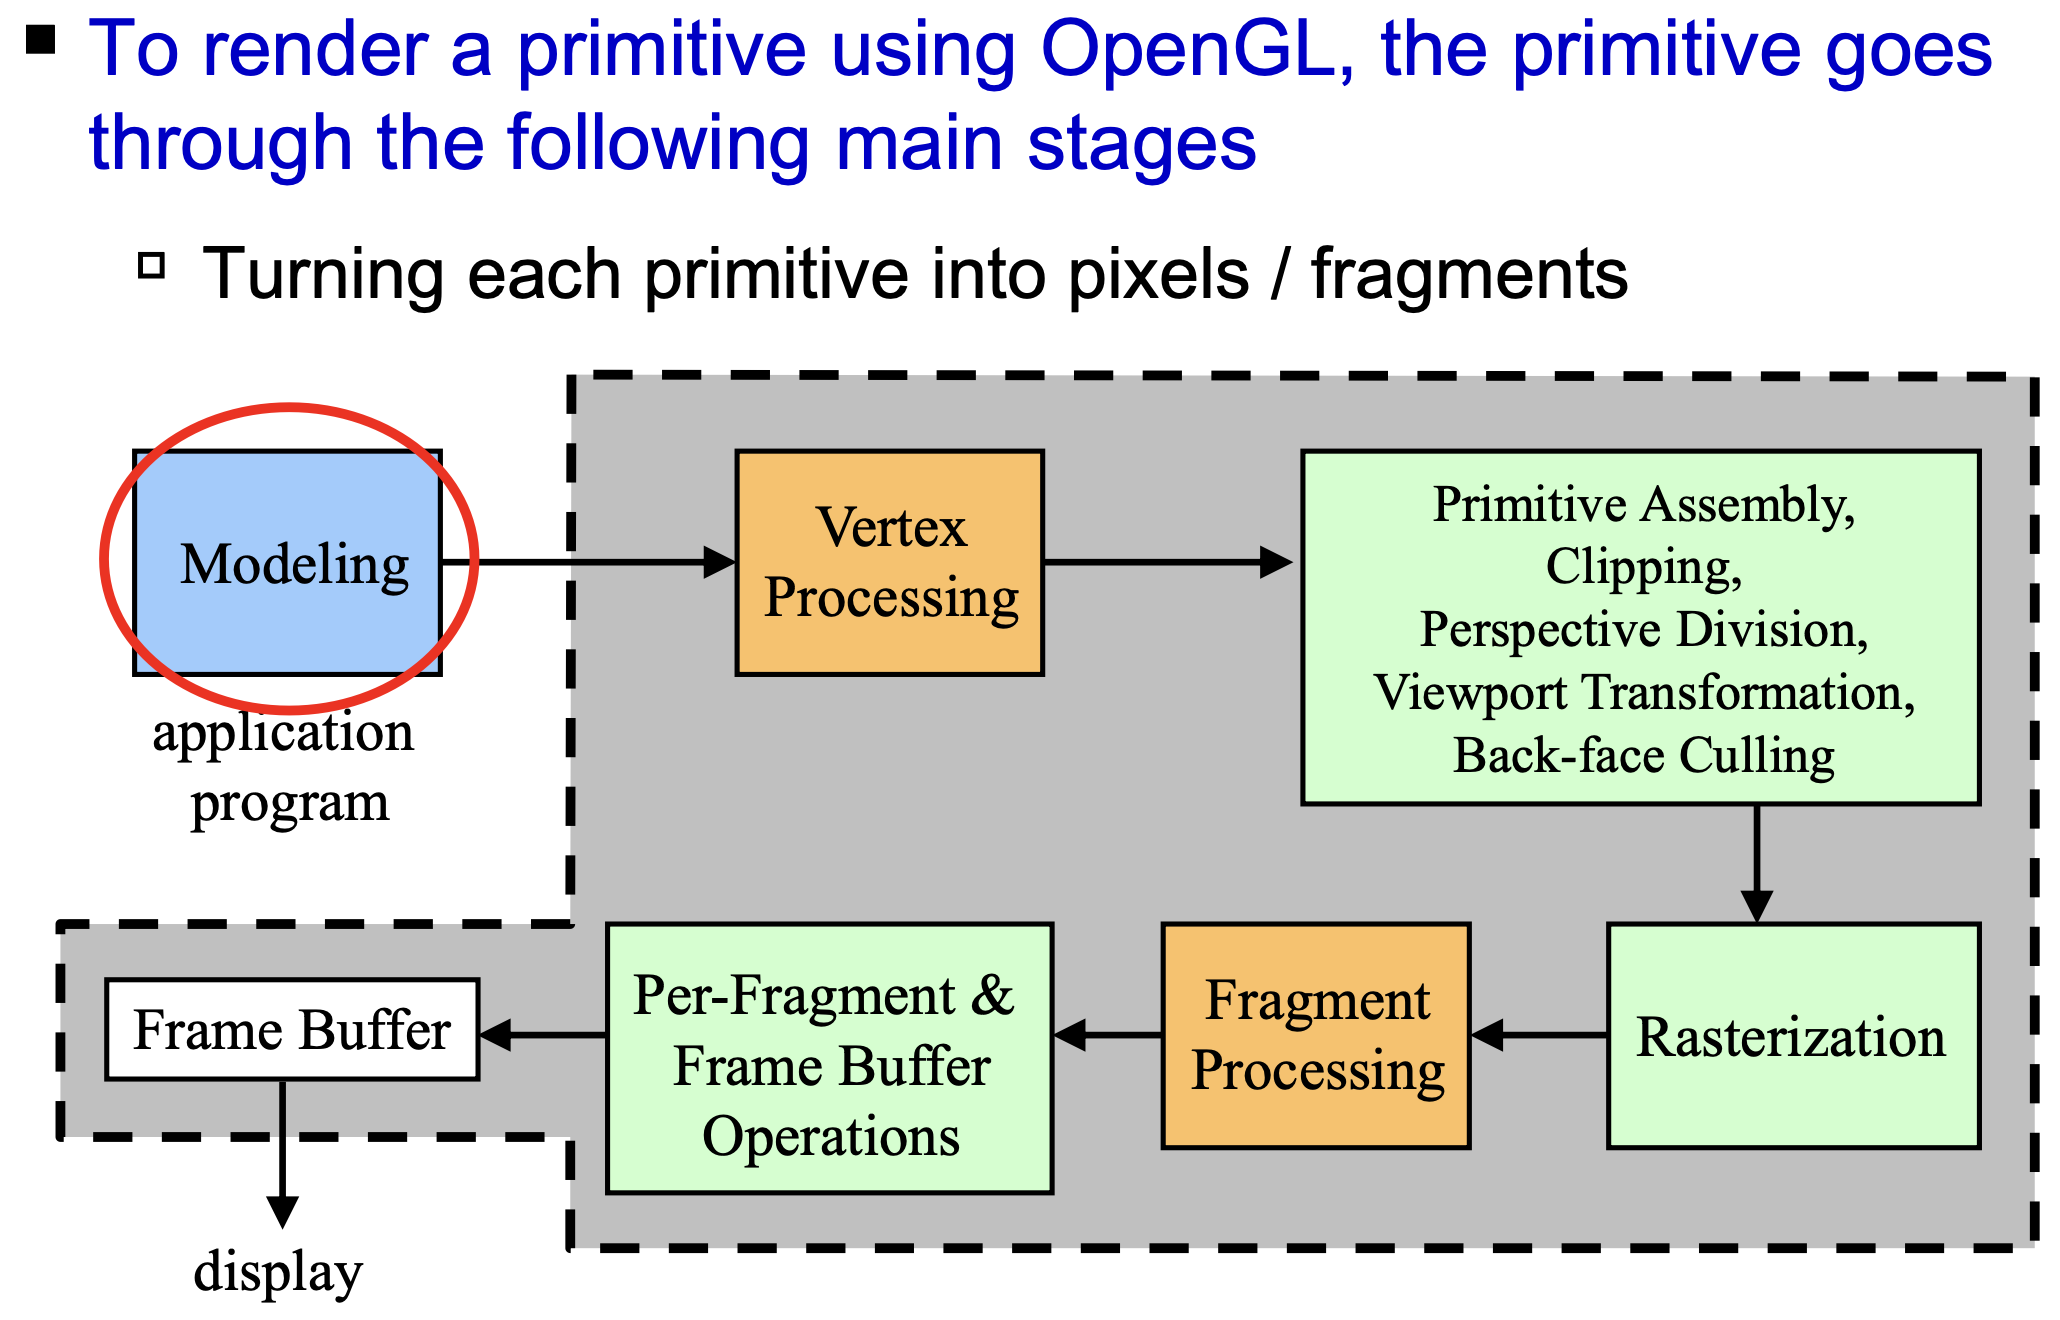
\includegraphics[width=0.8\columnwidth]{L6/rendering-pipeline}
  \end{center}
  \subsubsection*{Modelling}
    \begin{itemize}[leftmargin=*]
      \item Performed in application
      \item Provides a set of vertices that specifies geometric objects
      \item May perform scene processing to reduce amount of geometric data passed to rendering pipeline
        \begin{itemize}[leftmargin=*]
          \item View-frustum culling: do not pass objects that are outside the frustum
          \item Occlusion culling: do not pass objects that are completely blocked
        \end{itemize}
    \end{itemize}
\end{multicols*}
\begin{multicols*}{3}
  \subsubsection*{Vertex processing}
    \begin{itemize}[leftmargin=*]
      \item In this stage, model-view transformation is applied (now in camera/eye space), affecting vertices and vertex normals
      \item Assigns color to vertices using lighting computation
      \item Compute texture coordinates at vertices
      \item Projection matrix is applied (now in clip space)
    \end{itemize}
    \subsubsection*{Primitive assembly}
      \begin{itemize}[leftmargin=*]
        \item Primitive assembly
          \begin{itemize}[leftmargin=*]
            \item Vertex data was processed separately in previous vertex processing stage
            \item Vertex data is collected into complete primitives
            \item Necessary for clipping, rasterization, back face culling
          \end{itemize}
        \item Clipping
        \item Perspecive division (to NDC space)
        \item Viewport transformation (to window space, include depth-range scaling)
          \begin{itemize}[leftmargin=*]
            \item For rasterization to color specific pixels in the window
          \end{itemize}
        \item Back-face culling
      \end{itemize}
    \subsubsection*{Rasterization}
      \begin{itemize}[leftmargin=*]
        \item If geometric primitive not clipped out, appropriate pixels in frame buffer must be assigned colors
        \item Rasterizer produces a set of fragments for each primitive
          \begin{itemize}[leftmargin=*]
            \item Fragments are potential pixels, which have a pixel location, color, depth attributes
          \end{itemize}
        \item Vertex attributes are interpolated over the primitive
        \item In bilinear interpolation, take weighted average of endpoints on a line segment
      \end{itemize}
      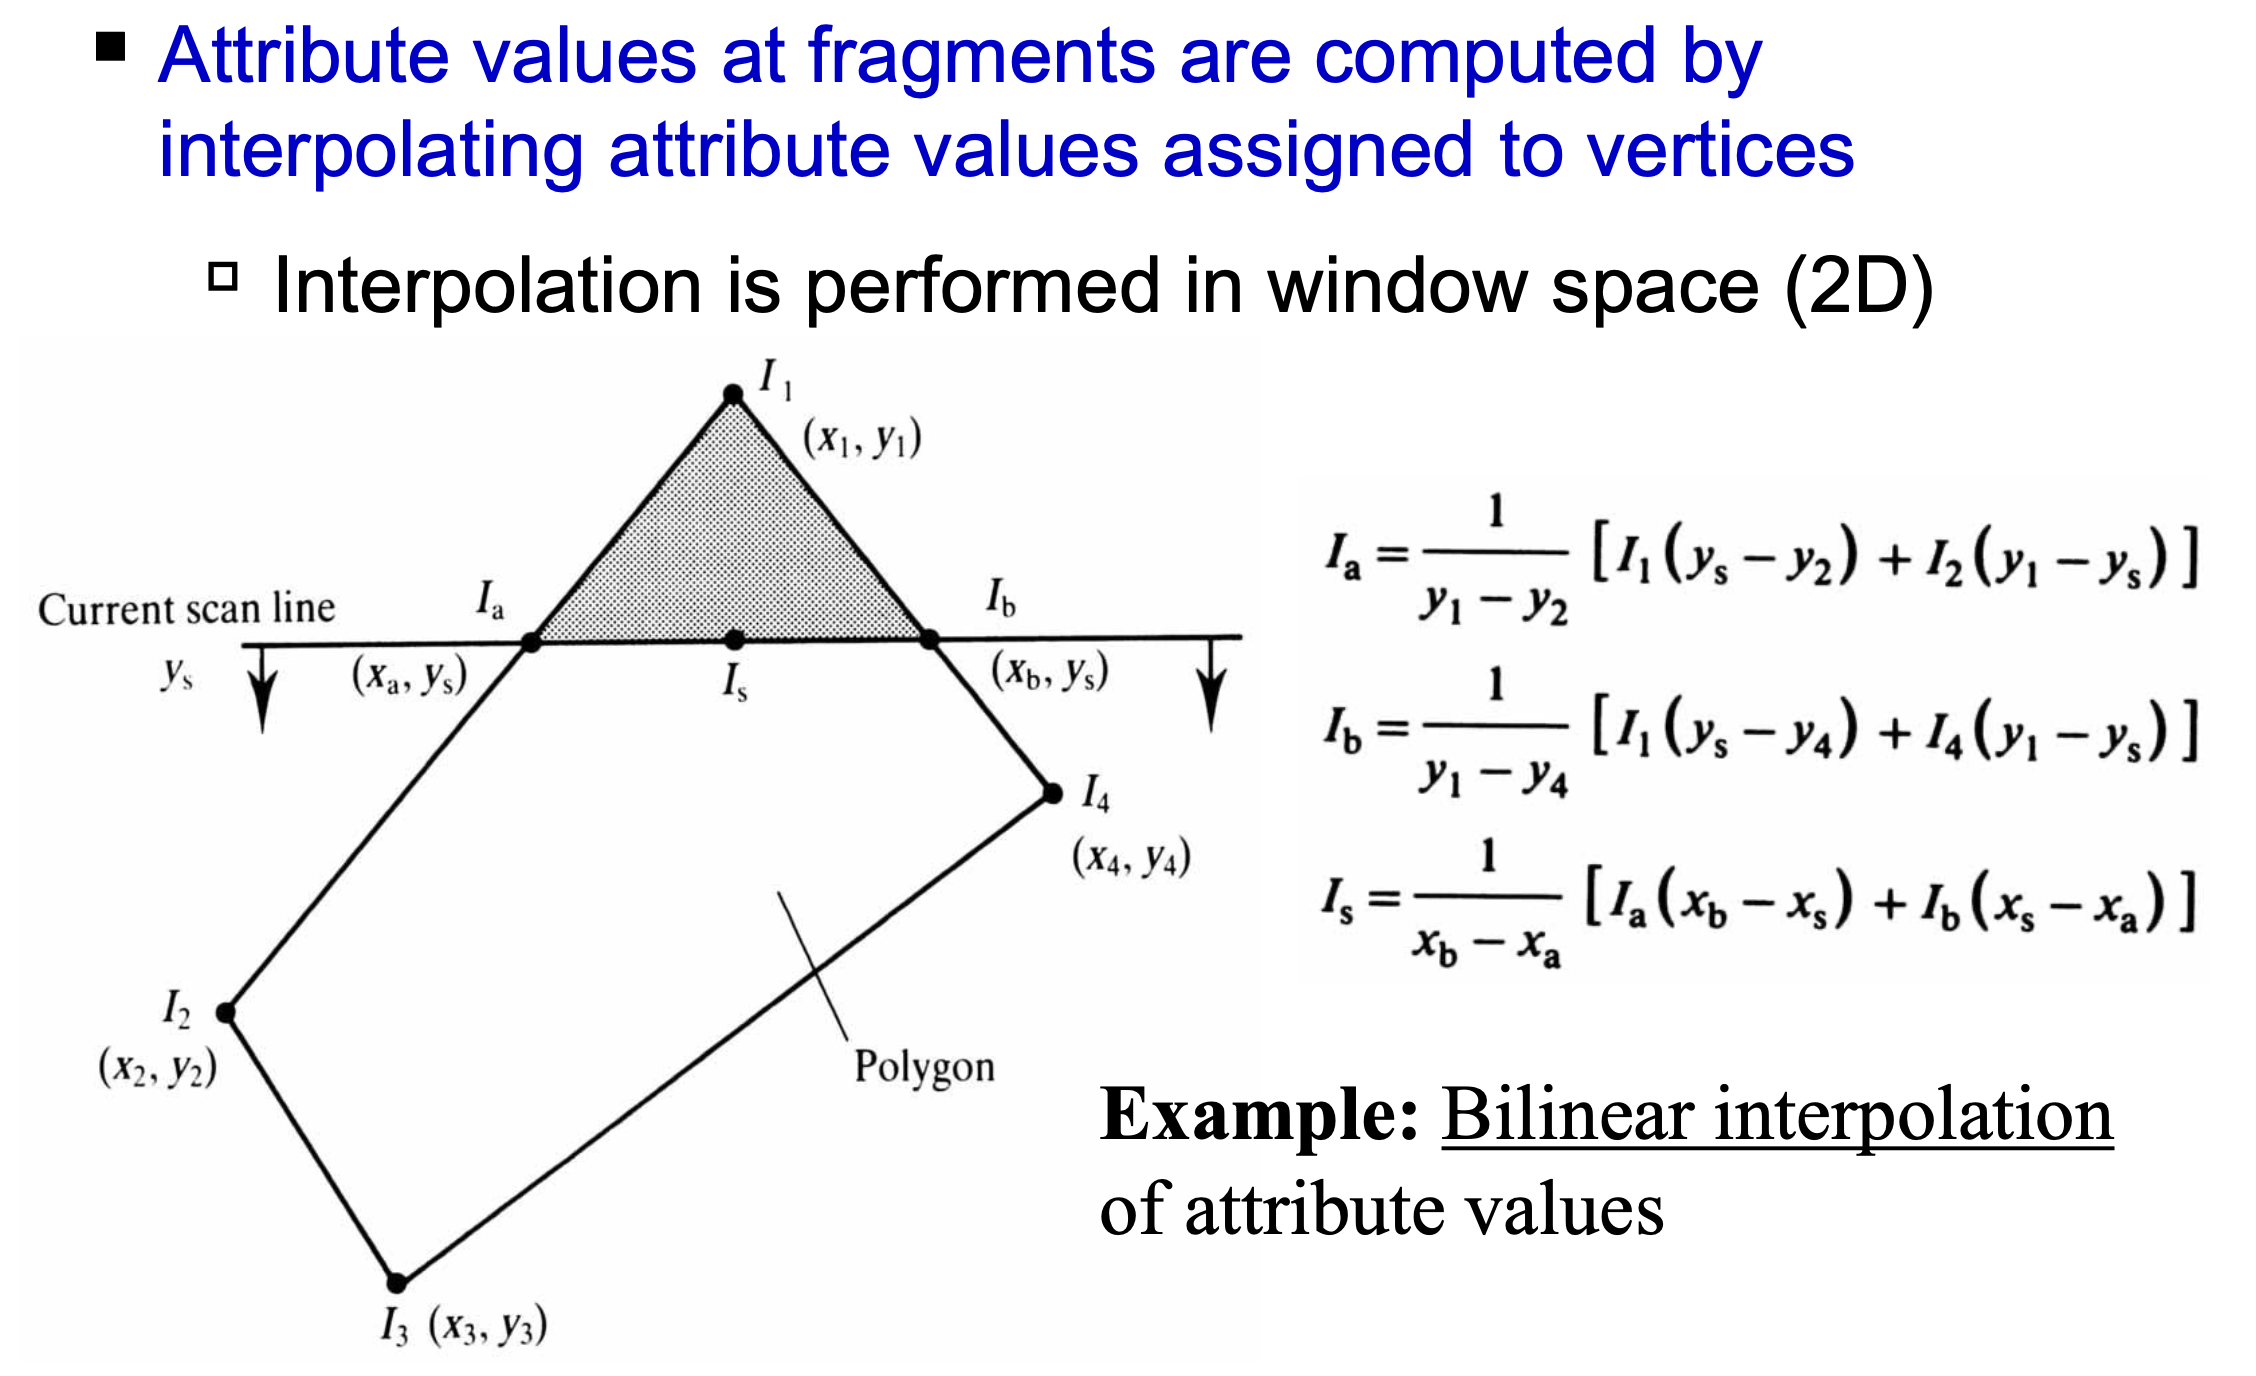
\includegraphics[width=\columnwidth]{L6/bilinear-interpolation}
      \begin{itemize}[leftmargin=*]
        \item Color interpolation
      \end{itemize}
      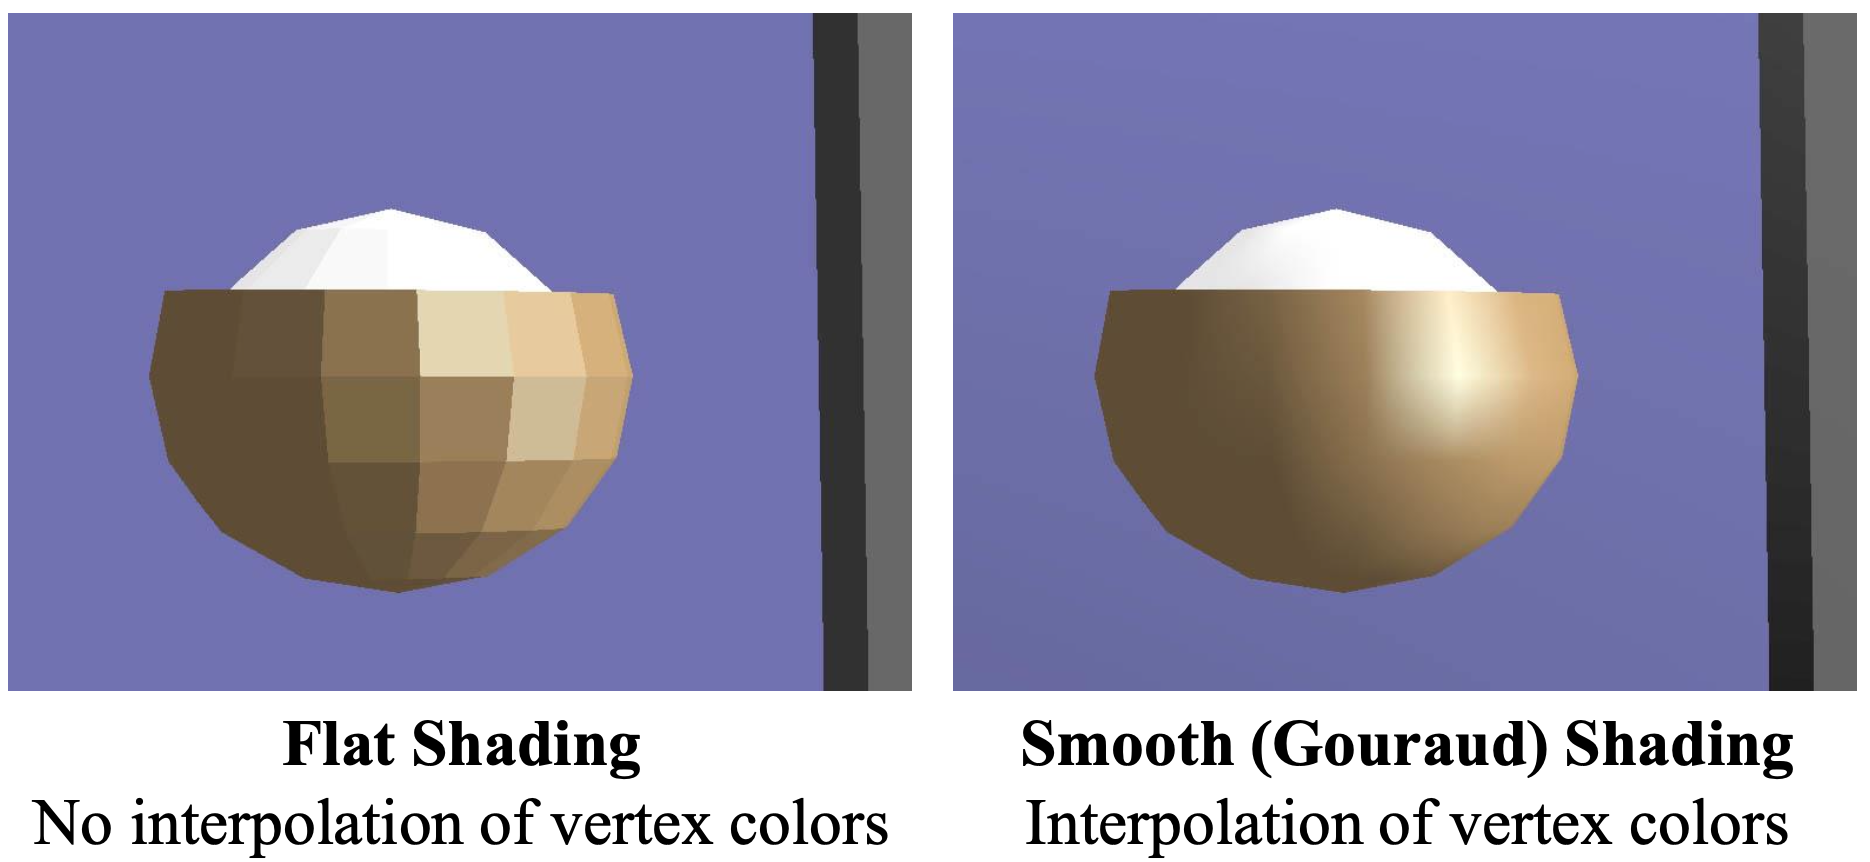
\includegraphics[width=\columnwidth]{L6/color-interpolation}
      \begin{itemize}[leftmargin=*]
        \item Can also interpolate $z$-value (depth), or texture coordinates
      \end{itemize}
    \subsubsection*{Fragment processing}
      \begin{itemize}[leftmargin=*]
        \item Each generated fragment is processed to determine the color of the corresponding pixel in the frame buffer
        \item Fragment color can be modified by texture mapping
          \begin{itemize}[leftmargin=*]
            \item Texture access (use the texture directly)
            \item Texture application (combine texture with fragment color)
          \end{itemize}
      \end{itemize}
    \subsubsection*{Per-fragment operations}
      \paragraph{Z-buffer hidden surface removal} Discard fragment if it is blocked (occluded) by corresponding pixel in frame buffer
      \paragraph{Blending} Blend fragment with corresponding pixel in frame buffer
\section*{Clipping}
  \begin{itemize}[leftmargin=*]
    \item Easy for line segments and polygons
    \item Hard for curves and text - convert to lines and polygons first
  \end{itemize}
  \subsection*{Clipping 2D line segments}
    \subsubsection*{Brute force}
      \begin{itemize}[leftmargin=*]
        \item Compute intersections with all side of clipping window
        \item Inefficient: one division per intersection
        \item Alternatives: Cohen-Sutherland, Liang-Barsky line clipping algorithms
      \end{itemize}
  \subsection*{Cohen-Sutherland} \noindent
    \subsubsection*{Split window into distinct regions} \noindent
      Extend sides of clipping window to get 9 distinct regions
      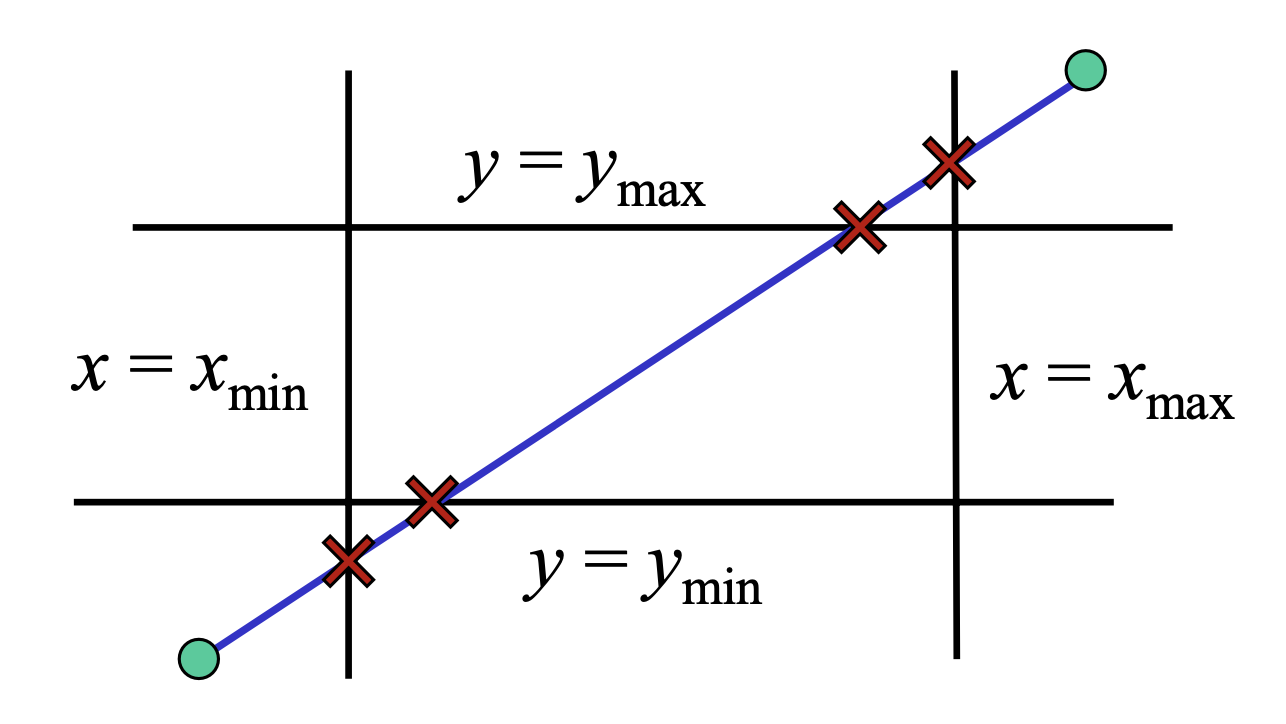
\includegraphics[width=\columnwidth]{L6/cohen-sutherland/9-regions}
    \subsubsection*{4 cases}
      \begin{enumerate}[leftmargin=*]
        \item Both endpoints inside all four lines - Accept
        \item Both endpoints outside same line - Reject
      \end{enumerate}
      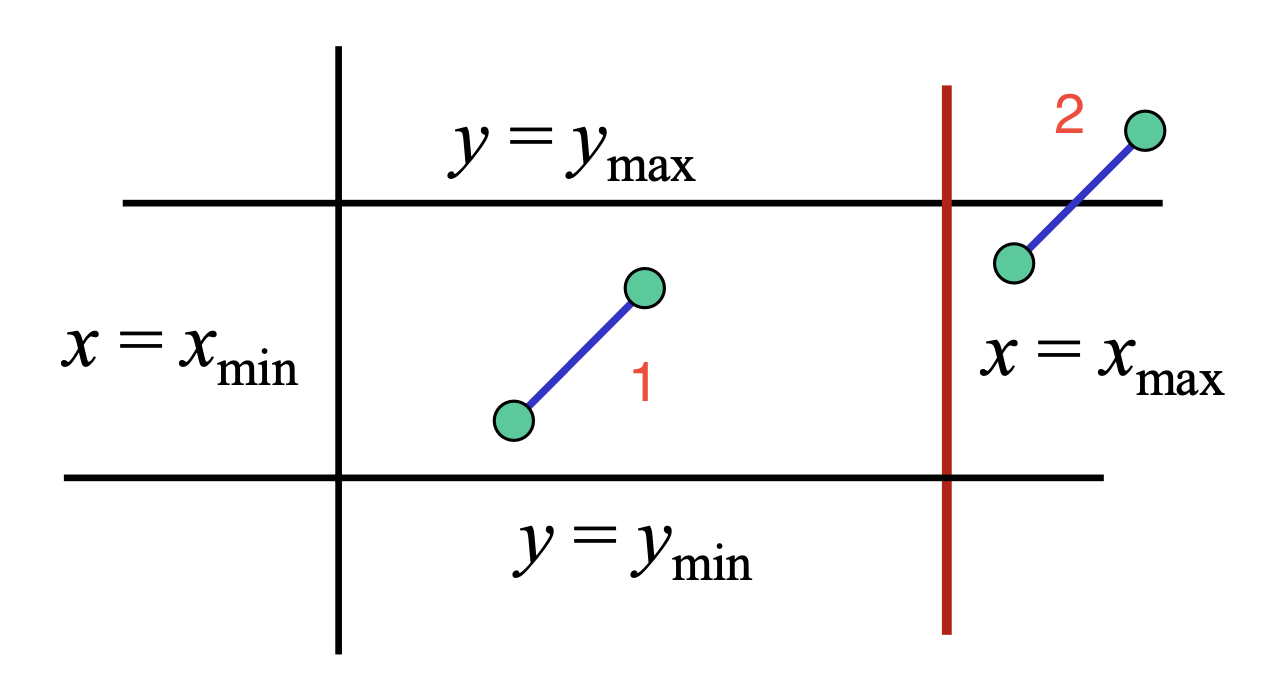
\includegraphics[width=\columnwidth]{L6/cohen-sutherland/case-1-2}
      \begin{enumerate}[leftmargin=*, resume]
        \item One endpoint inside all four lines, one outside - Perform intersection
        \item Both outside $\Rightarrow$ may have some part inside. Do one intersection, reducing to Case 2 or Case 3.
      \end{enumerate}
      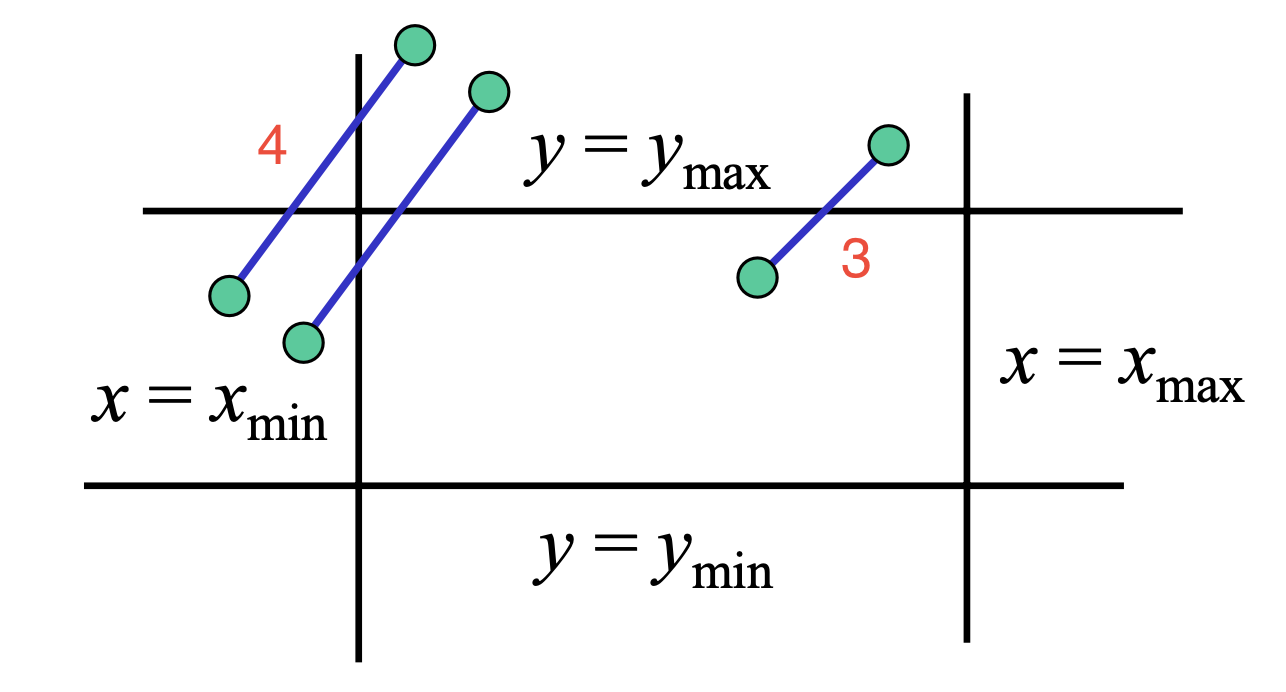
\includegraphics[width=\columnwidth]{L6/cohen-sutherland/case-3-4}
    \subsubsection*{Outcodes}
      \begin{itemize}[leftmargin=*]
        \item Define outcodes for easier computation
          \begin{itemize}[leftmargin=*]
            \item Outcodes divide space into 9 regions
            \item Computation of outcode requires at most 4 subtractions
          \end{itemize}
      \end{itemize}
      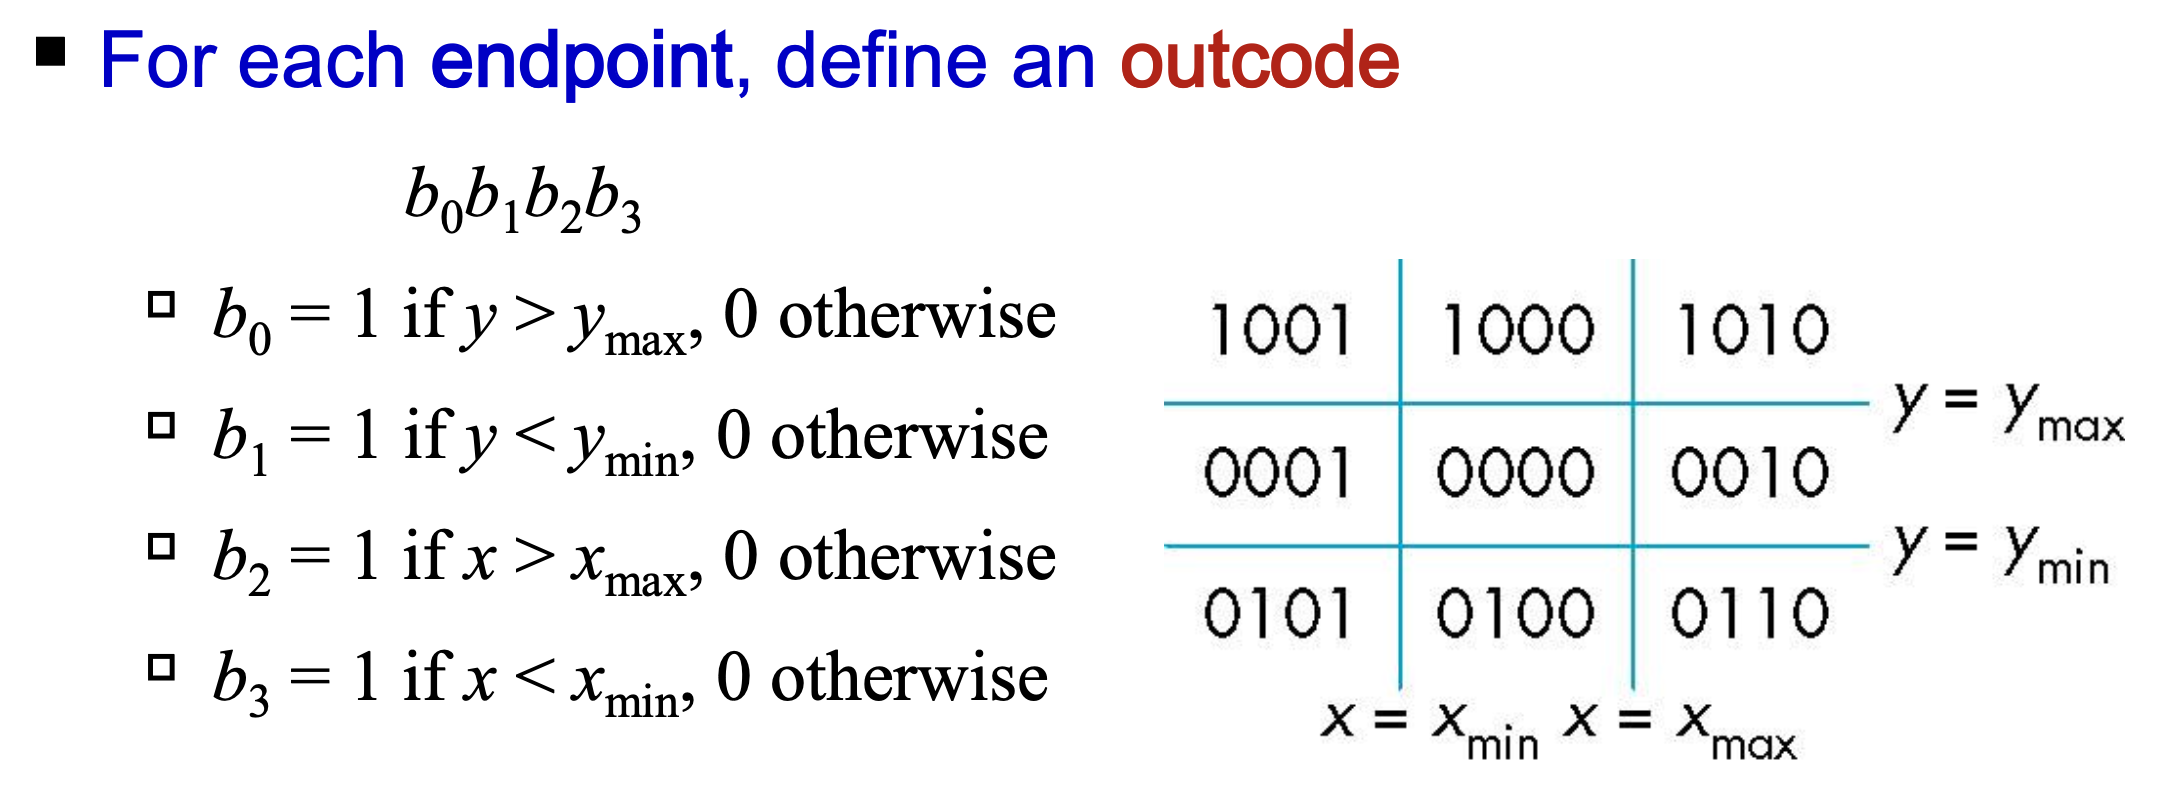
\includegraphics[width=\columnwidth]{L6/cohen-sutherland/outcodes}
      Consider line segment AB
      \begin{itemize}[leftmargin=*]
        \item Case 1: outcodes are both 0
          \begin{itemize}[leftmargin=*]
            \item Accepted
          \end{itemize}
        \item Case 2: outcode A AND outcode B (bitwise) is not 0
          \begin{itemize}[leftmargin=*]
            \item Both outcodes have 1 in same bit location (i.e. both outside the same line)
            \item Rejected
          \end{itemize}
        \item Case 3: outcode A is 0, outcode B not 0
          \begin{itemize}[leftmargin=*]
            \item Compute intersection, by using the location of 1 in outcode B
            \item If outcode D has more two 1s, then do two intersections
          \end{itemize}
        \item Case 4: Neither 0, logical AND yields 0
          \begin{itemize}[leftmargin=*]
            \item Shorten line segment by intersecting with one side of window
            \item Compute outcode of new line segment
            \item Repeat algorithm. Yields case 2 or case 3
          \end{itemize}
      \end{itemize}
    \subsubsection*{Efficiency}
      \begin{itemize}[leftmargin=*]
        \item Clipping window is usually small, relative to the entire database of line segments
        \item Most line segments are outside one or more sides of the window, and can be eliminated early
        \item Inefficient if case 4 occurs often
      \end{itemize}
    \subsubsection*{Application to 3D}
      \begin{itemize}[leftmargin=*]
        \item Use 6 bit outcodes
        \item Clip line segment against planes
      \end{itemize}
      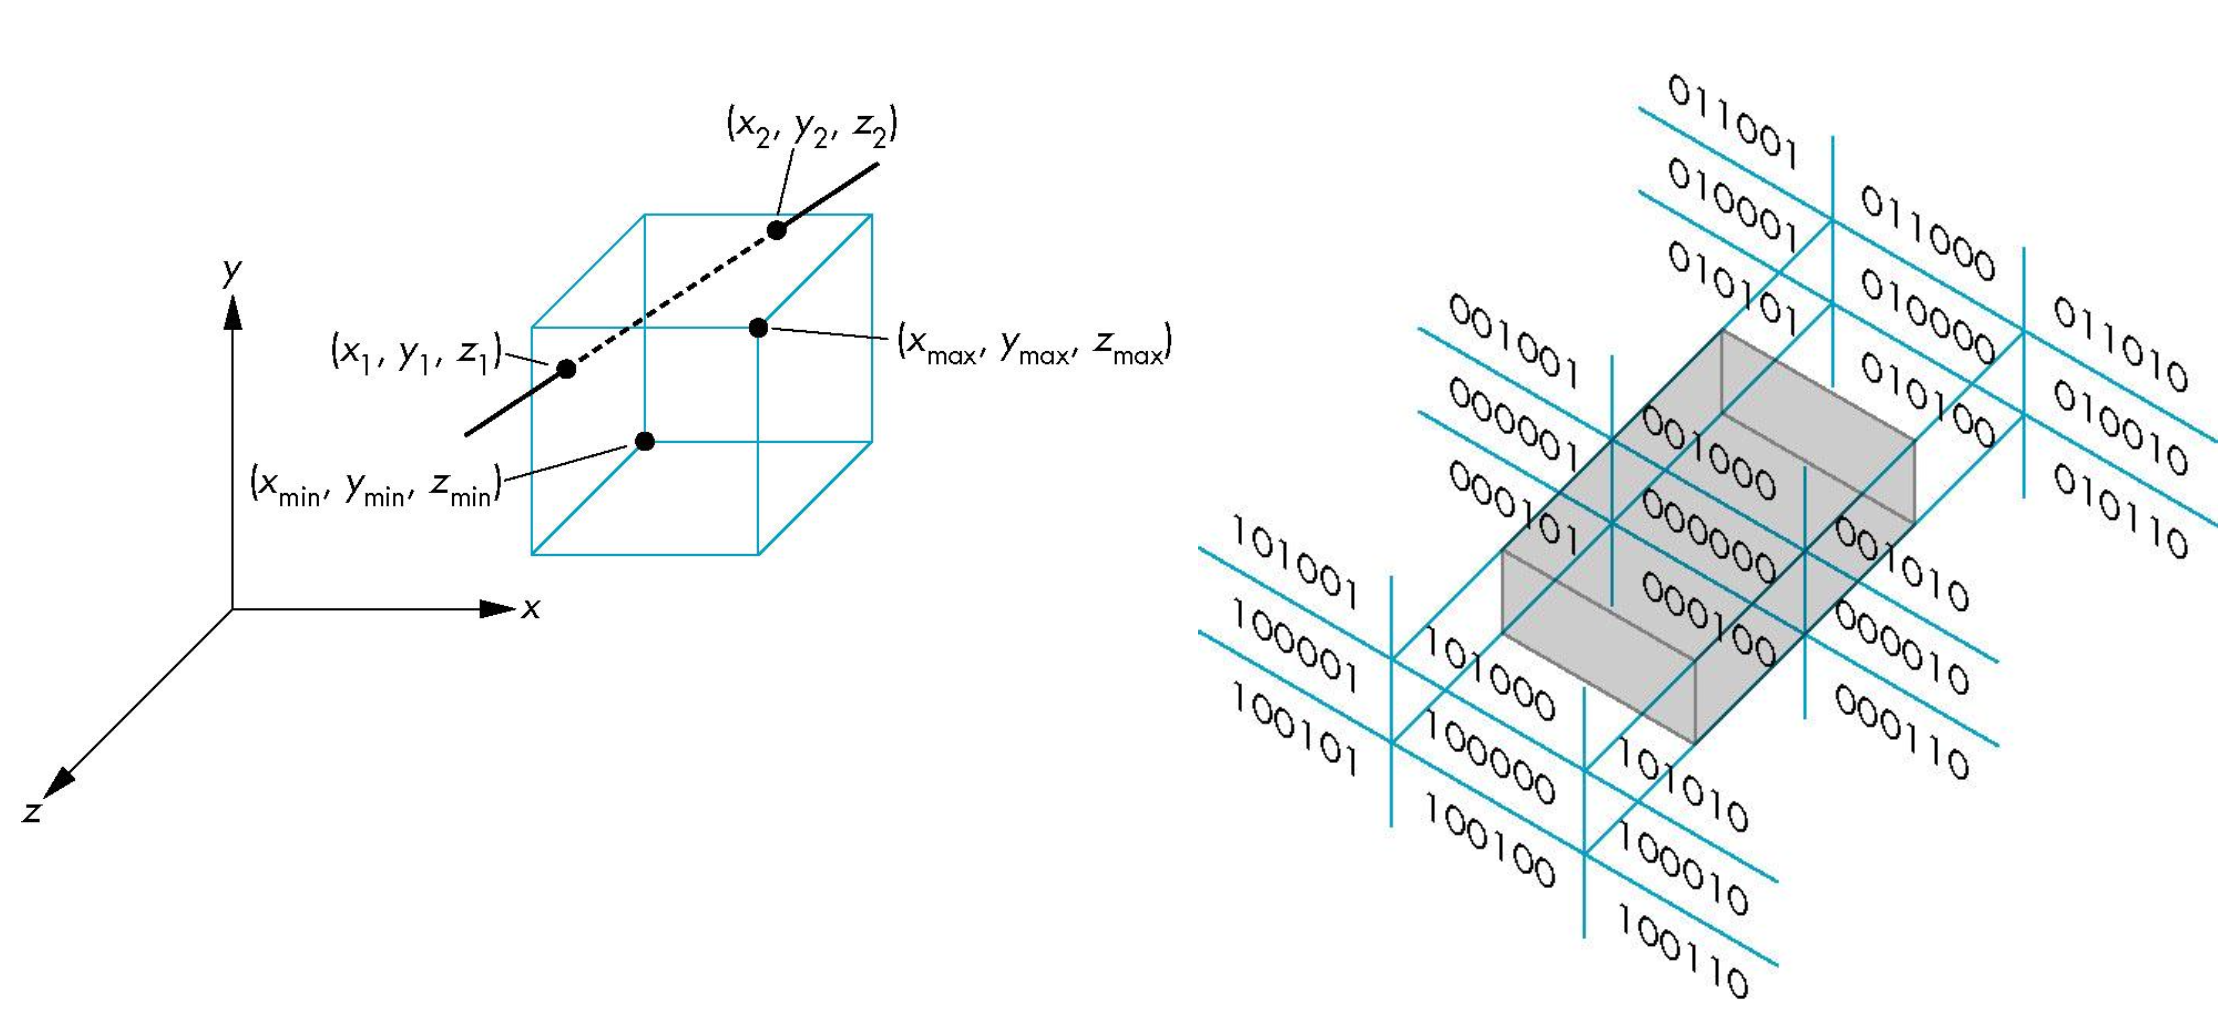
\includegraphics[width=\columnwidth]{L6/cohen-sutherland/3d}
  \subsection*{Misc}
    \subsubsection*{Clipping in clip space}
      \begin{itemize}[leftmargin=*]
        \item A vertex is in clip space after multiplication by projection matrix, and before perspective division
        \item Has coordinates $(x,y,z,w)$
        \item If vertex is in canonical view volume, then
          \begin{align*}
            -1 \leq x/w \leq 1 \quad &\Rightarrow \quad -w \leq x \leq w \\
            -1 \leq y/w \leq 1 \quad &\Rightarrow \quad -w \leq y \leq w \\
            -1 \leq z/w \leq 1 \quad &\Rightarrow \quad -w \leq z \leq w
          \end{align*}
        \item The 6 inequalities are used to decide whether a vertex should be clipped away, in clip space
      \end{itemize}
    \subsubsection*{Polygon clipping}
      \begin{itemize}[leftmargin=*]
        \item If convex, clipping yields at most one other polygon
        \item If concave, use tessellation to split the polygon into a set of smaller convex polygons
          \begin{itemize}[leftmargin=*]
            \item Usually use triangles
            \item Also makes rasterization easier
          \end{itemize}
      \end{itemize}
      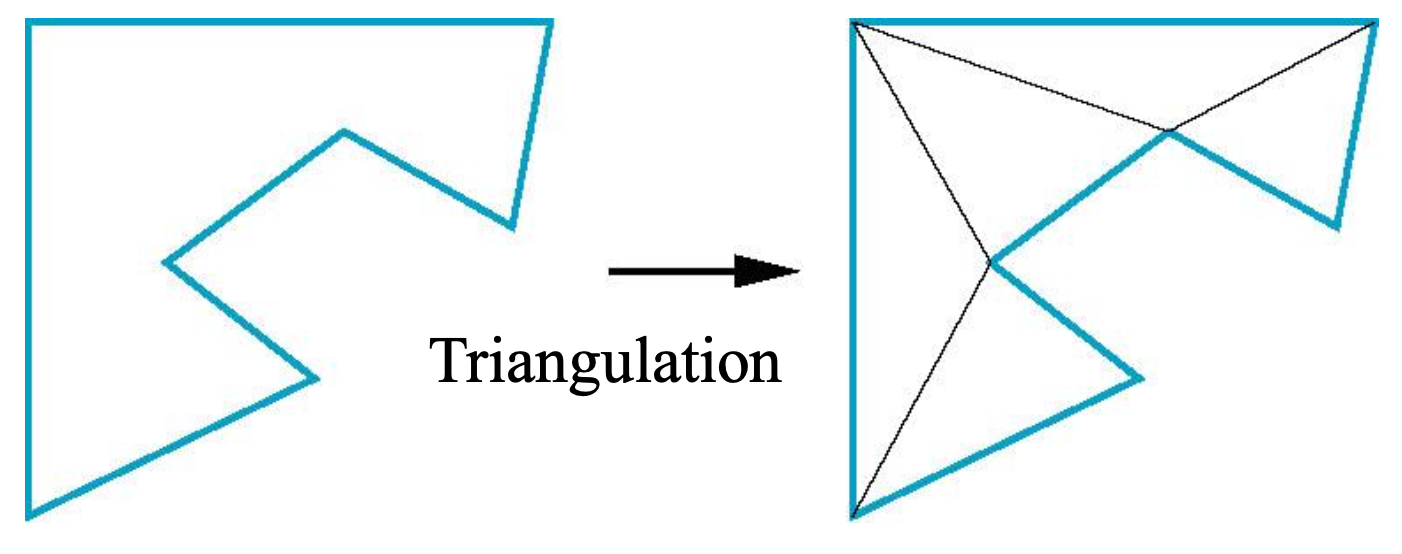
\includegraphics[width=\columnwidth]{L6/triangulation}
    \subsubsection*{Pipeline clipping of line segments}
      \begin{itemize}[leftmargin=*]
        \item Clipping against each side of window is independent of other sides
        \item Can use four independent clippers in pipeline
      \end{itemize}
    \subsubsection*{Simple early acceptance \& rejection}
      \begin{itemize}[leftmargin=*]
        \item Use an axis-aligned bounding box (AABB) instead of clipping a complex polygon
        \item AABB: smallest axis-aligned rectangle that encloses the polygon
        \item Simple to compute: max and min of $x$ and $y$
      \end{itemize}
      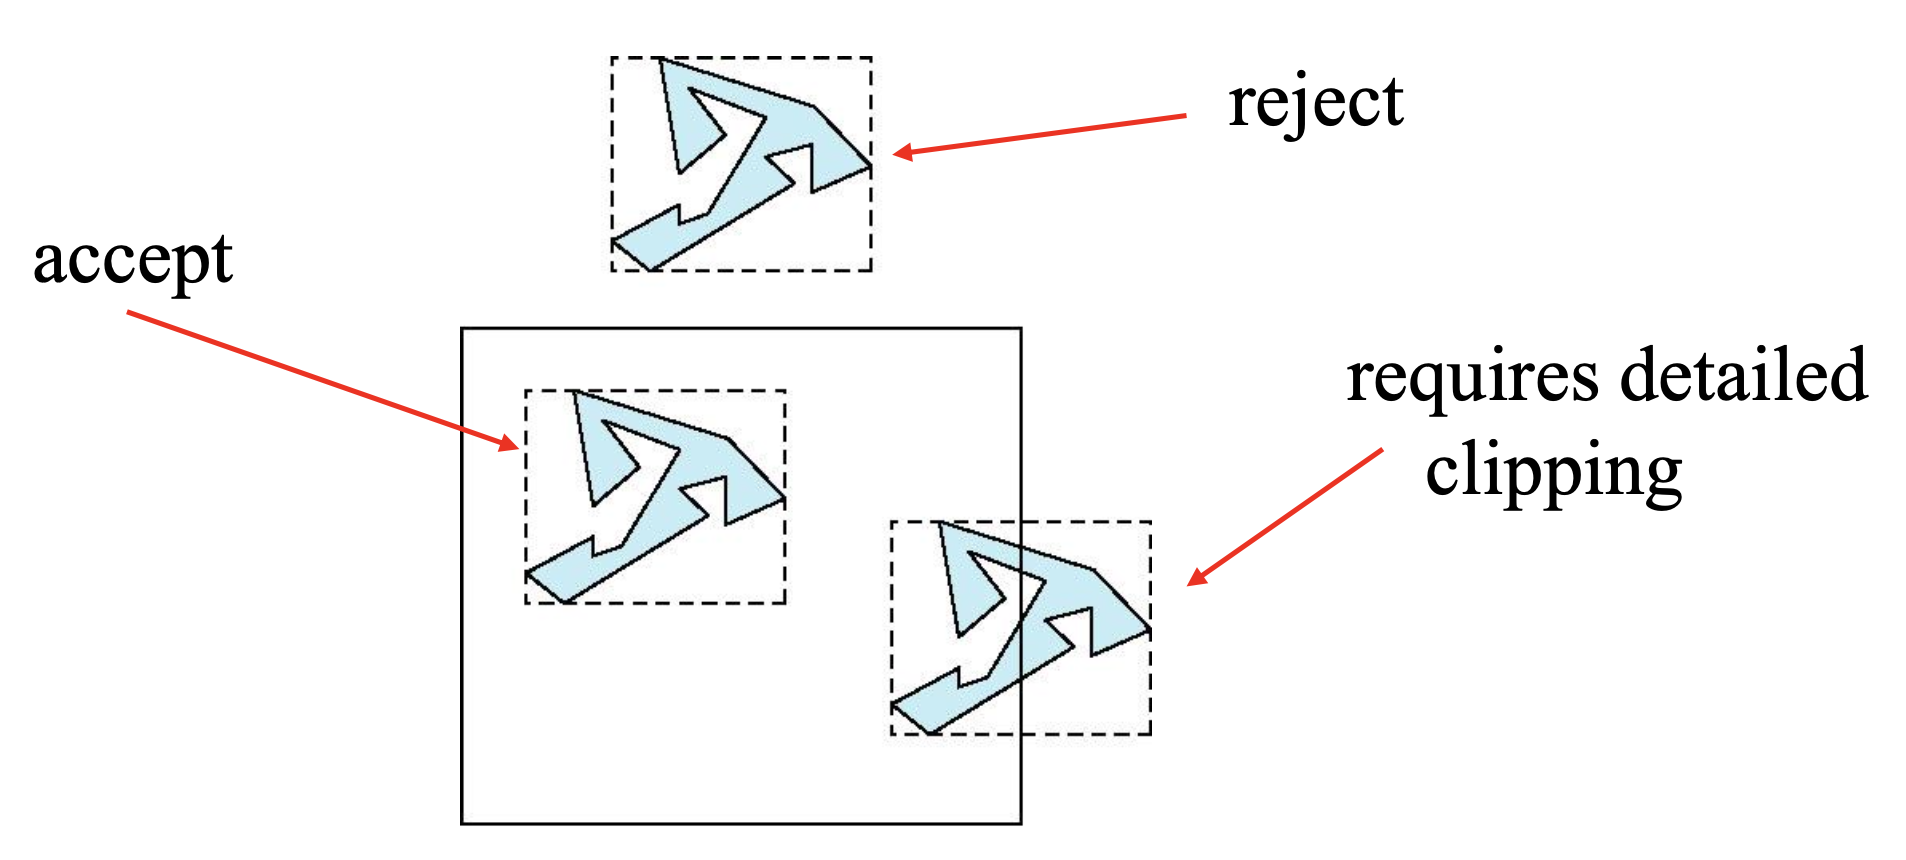
\includegraphics[width=\columnwidth]{L6/aabb}
\section*{Rasterization}
  \subsection*{Digital Differential Analyzer - DDA}
    \begin{itemize}[leftmargin=*]
      \item For every $x$, plot pixel at closest $y$
    \end{itemize}
    \begin{lstlisting}
for (x = x0, y = y0; x <= xe; x++) {
    write_pixel(x, round(y), line_color);
    y += m;
}
    \end{lstlisting}
    \subsubsection*{Steep lines}
      \begin{itemize}[leftmargin=*]
        \item Problem with steep lines, so use only when $0 \leq \abs{m} \leq 1$.
        \item For $\abs{m} > 1$, swap roles of $x$ and $y$, i.e. for every $y$, plot pixel at closest $x$
      \end{itemize}
      \begin{center}
        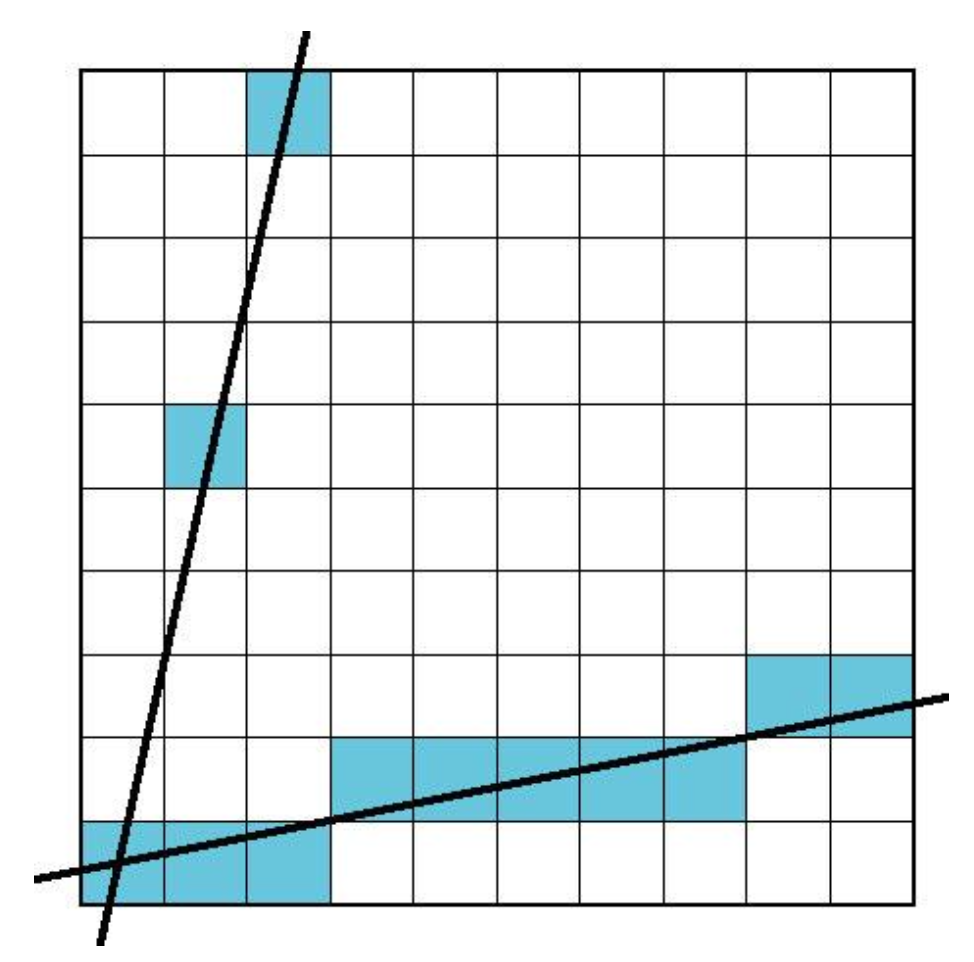
\includegraphics[width=0.6\columnwidth]{L6/dda}
      \end{center}
  \subsection*{Bresenham's Algorithm}
    \begin{itemize}[leftmargin=*]
      \item DDA requires one floating point addition per step
      \item Bresenham's algorithm can avoid floating point operations
      \item Consider only $0 \leq m \leq 1$, the rest can be derived by symmetry
        \begin{itemize}[leftmargin=*]
          \item Next pixel is either to the right, or right and top
          \item Turns into binary decision problem
        \end{itemize}
    \end{itemize}
    \begin{center}
      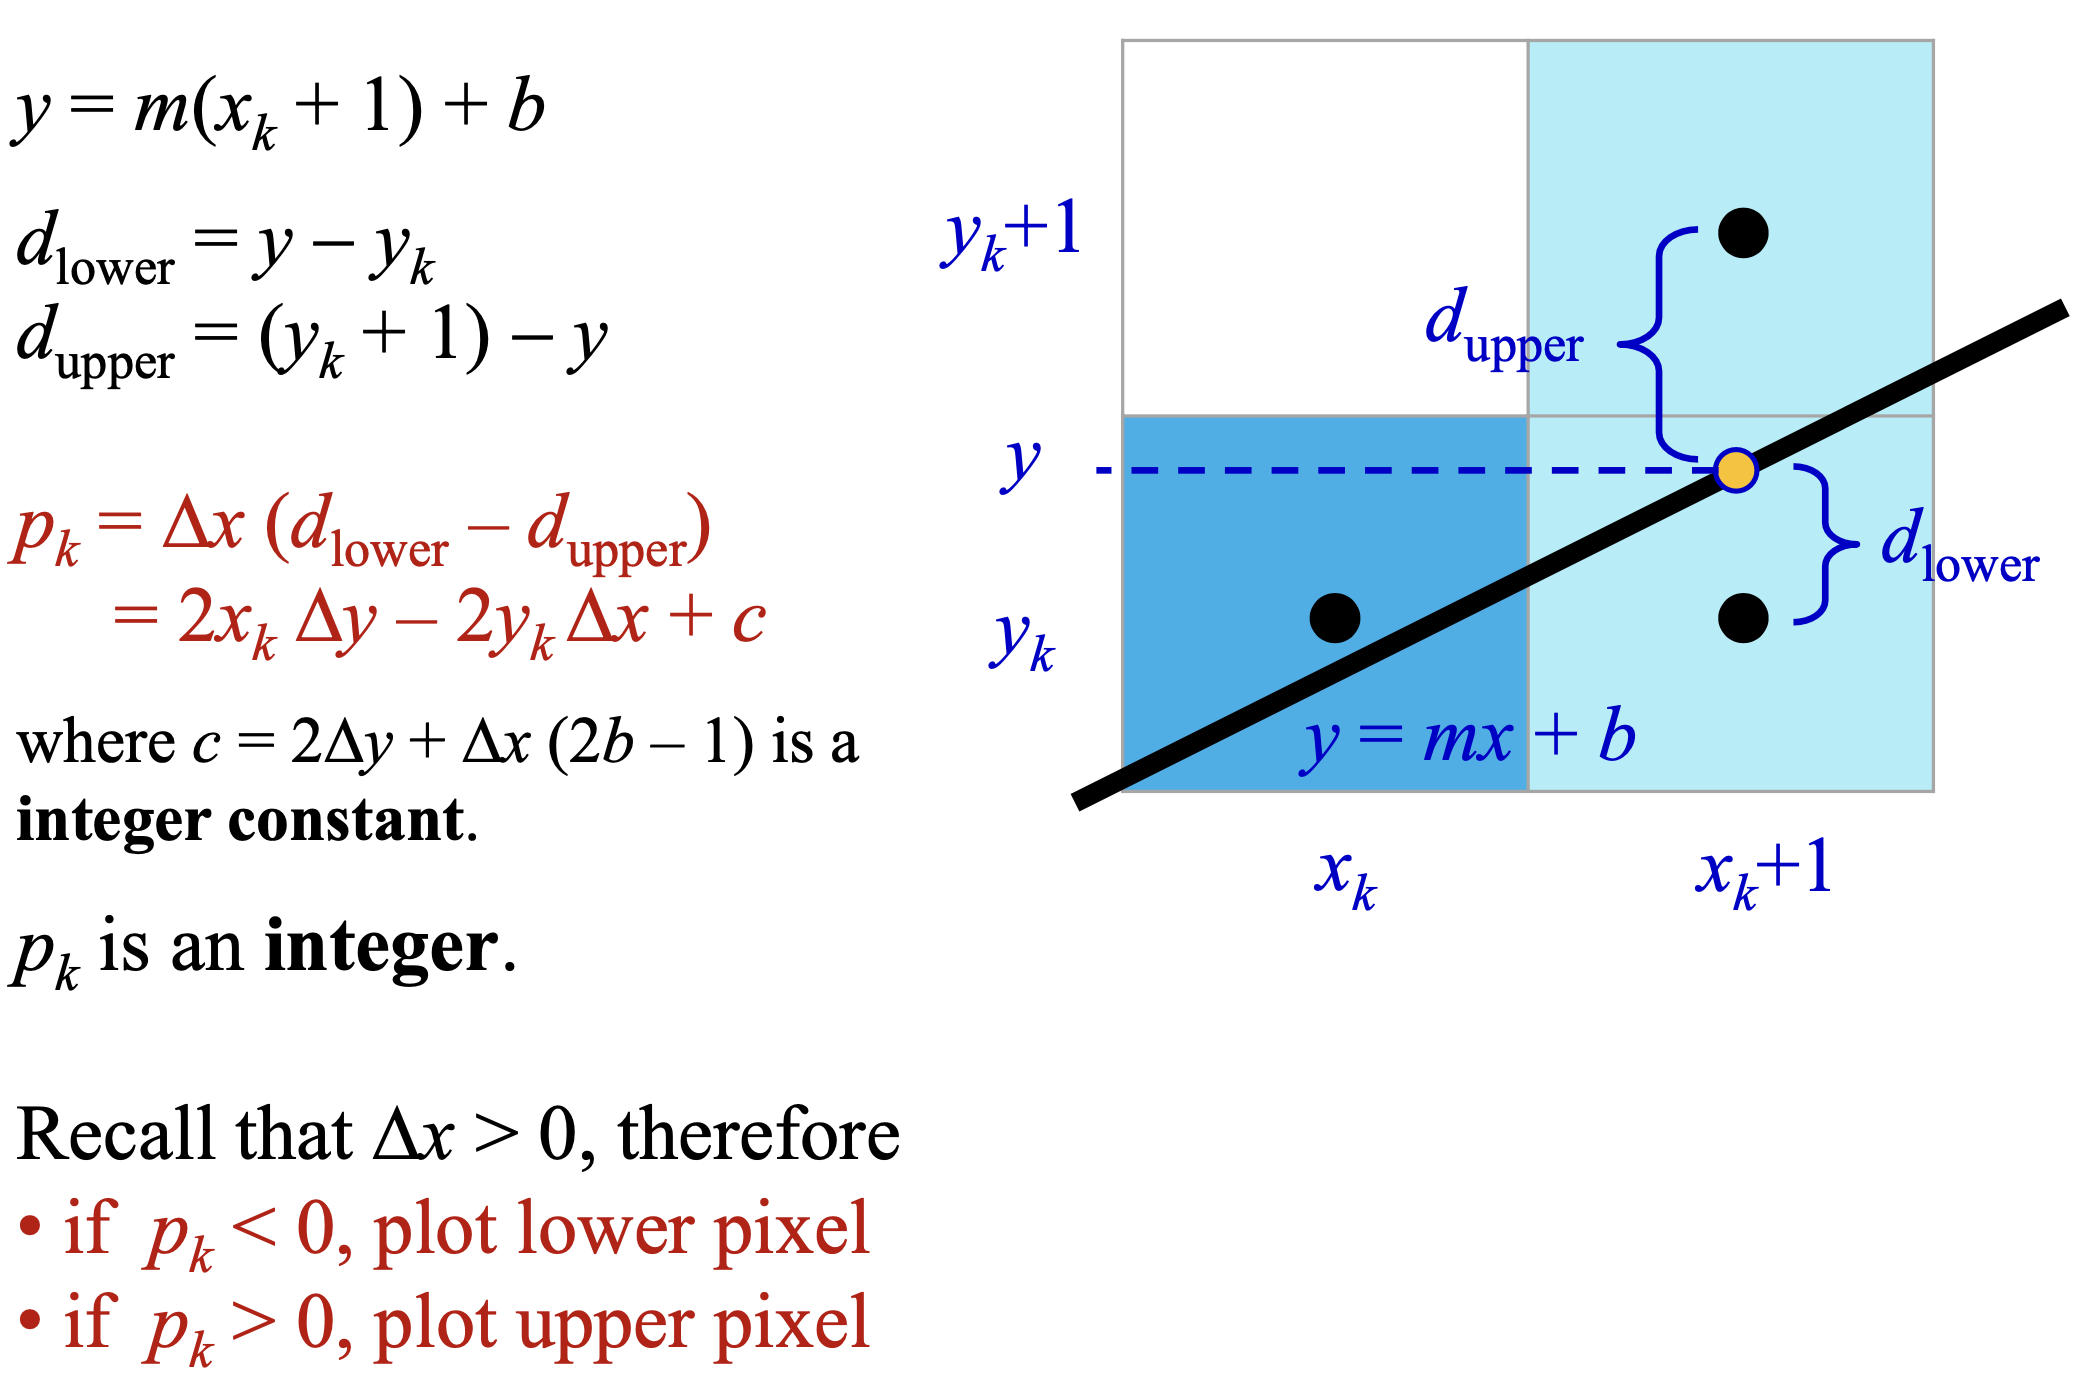
\includegraphics[width=\columnwidth]{L6/bresenham-1}
      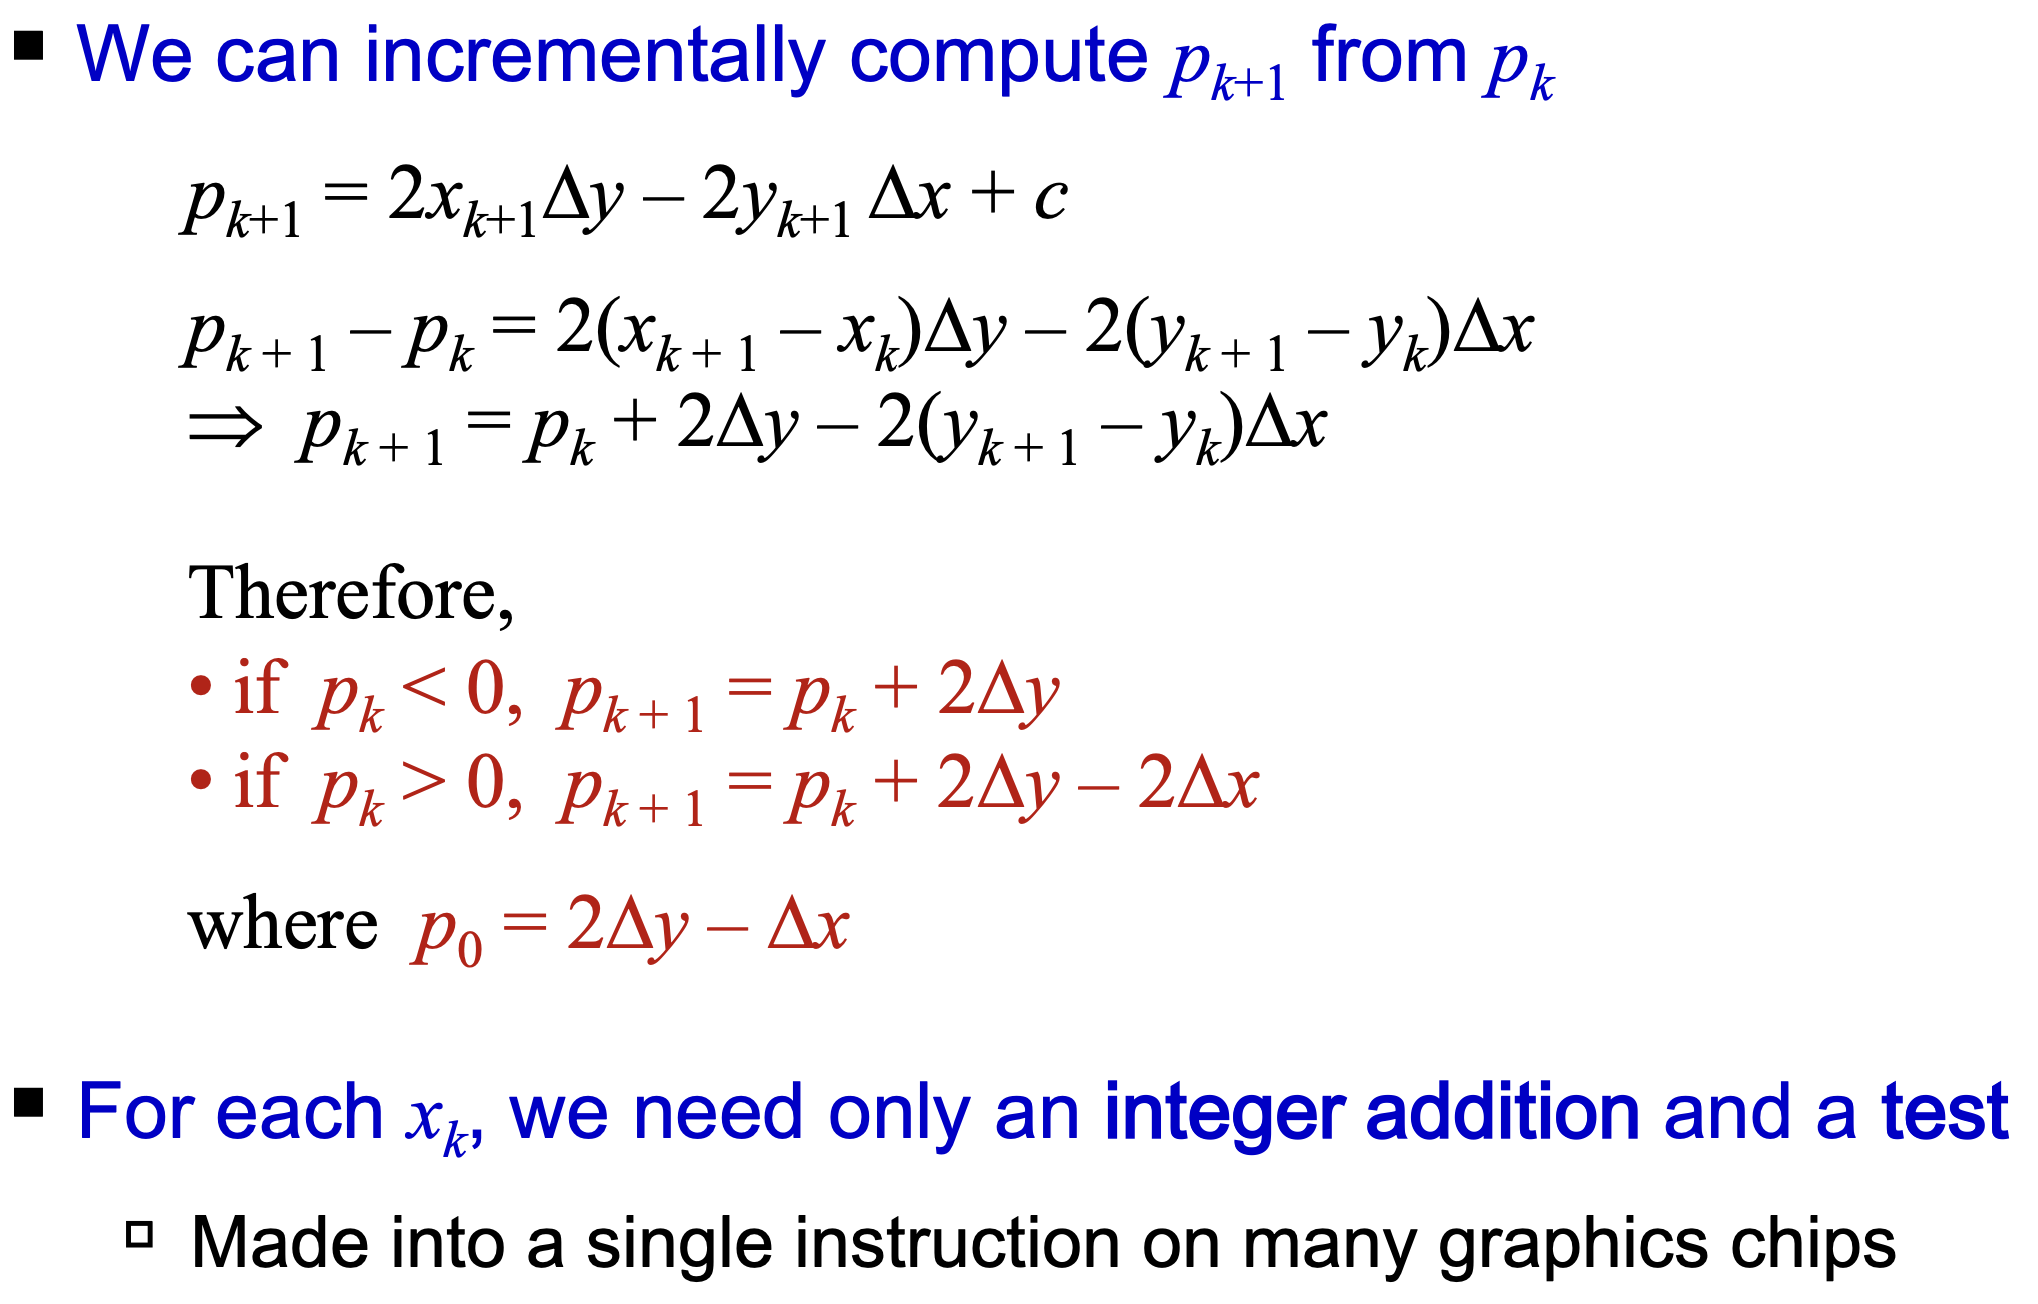
\includegraphics[width=\columnwidth]{L6/bresenham-2}
    \end{center}
  \subsection*{Scan-line fill}
    \begin{itemize}[leftmargin=*]
      \item Applies to convex polygons (usually triangles)
        \begin{itemize}[leftmargin=*]
          \item Non-convex polygons assumed tessellated
        \end{itemize}
      \item Shades (colors) have been computed for vertices
      \item Combine with $z$-buffer algorithm
        \begin{itemize}[leftmargin=*]
          \item Vertices also have $z$-values (depth-values)
        \end{itemize}
      \item March across horizontal scan lines, interpolating shades and $z$-values
    \end{itemize}
    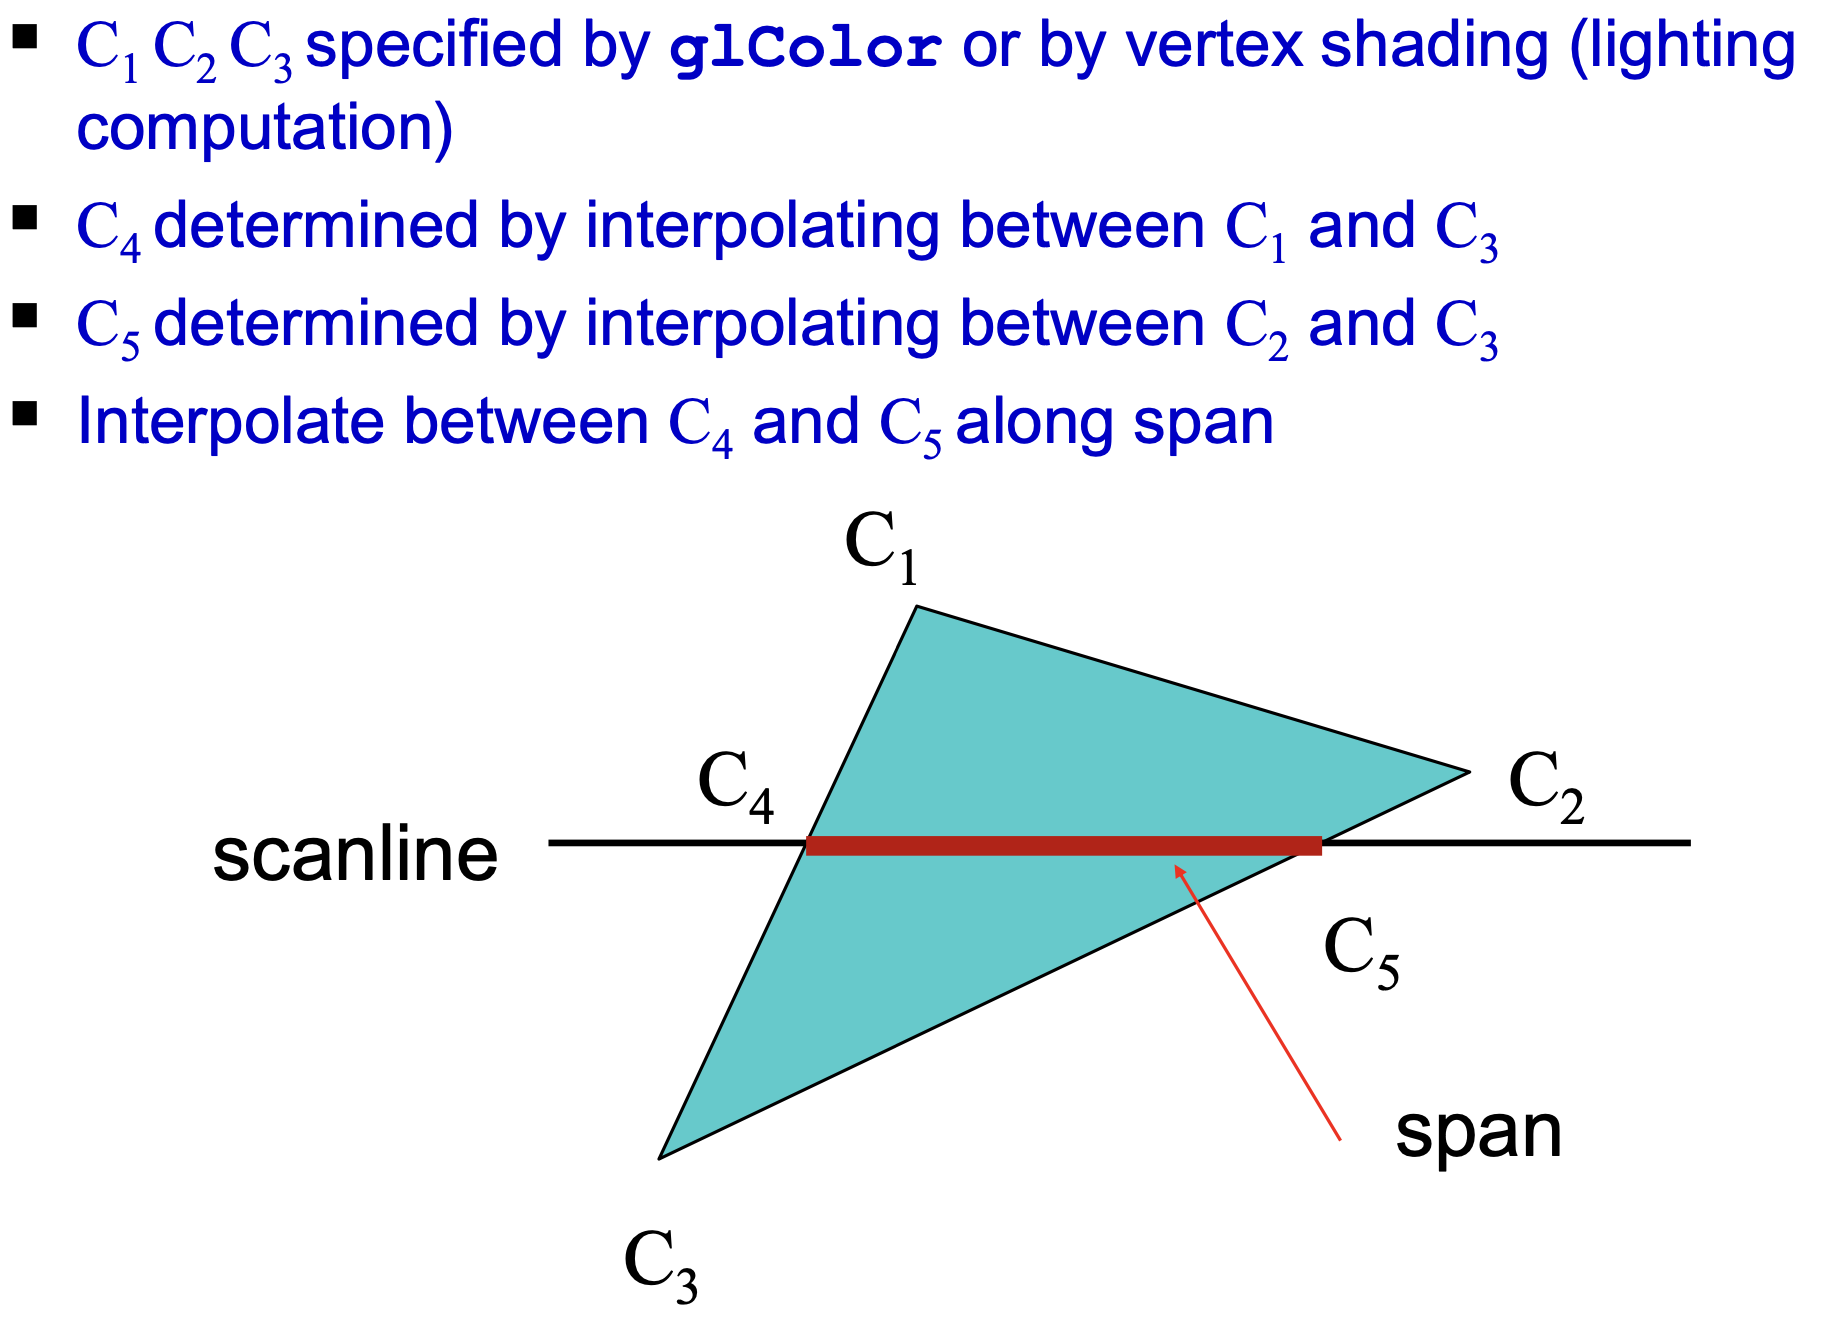
\includegraphics[width=\columnwidth]{L6/scan-line}
    \begin{itemize}[leftmargin=*]
      \item Can also fill by maintaining a data structure of all intersections of polygons with scanlines
        \begin{itemize}[leftmargin=*]
          \item Sort by scan line
          \item Fill each span
        \end{itemize}
    \end{itemize}
    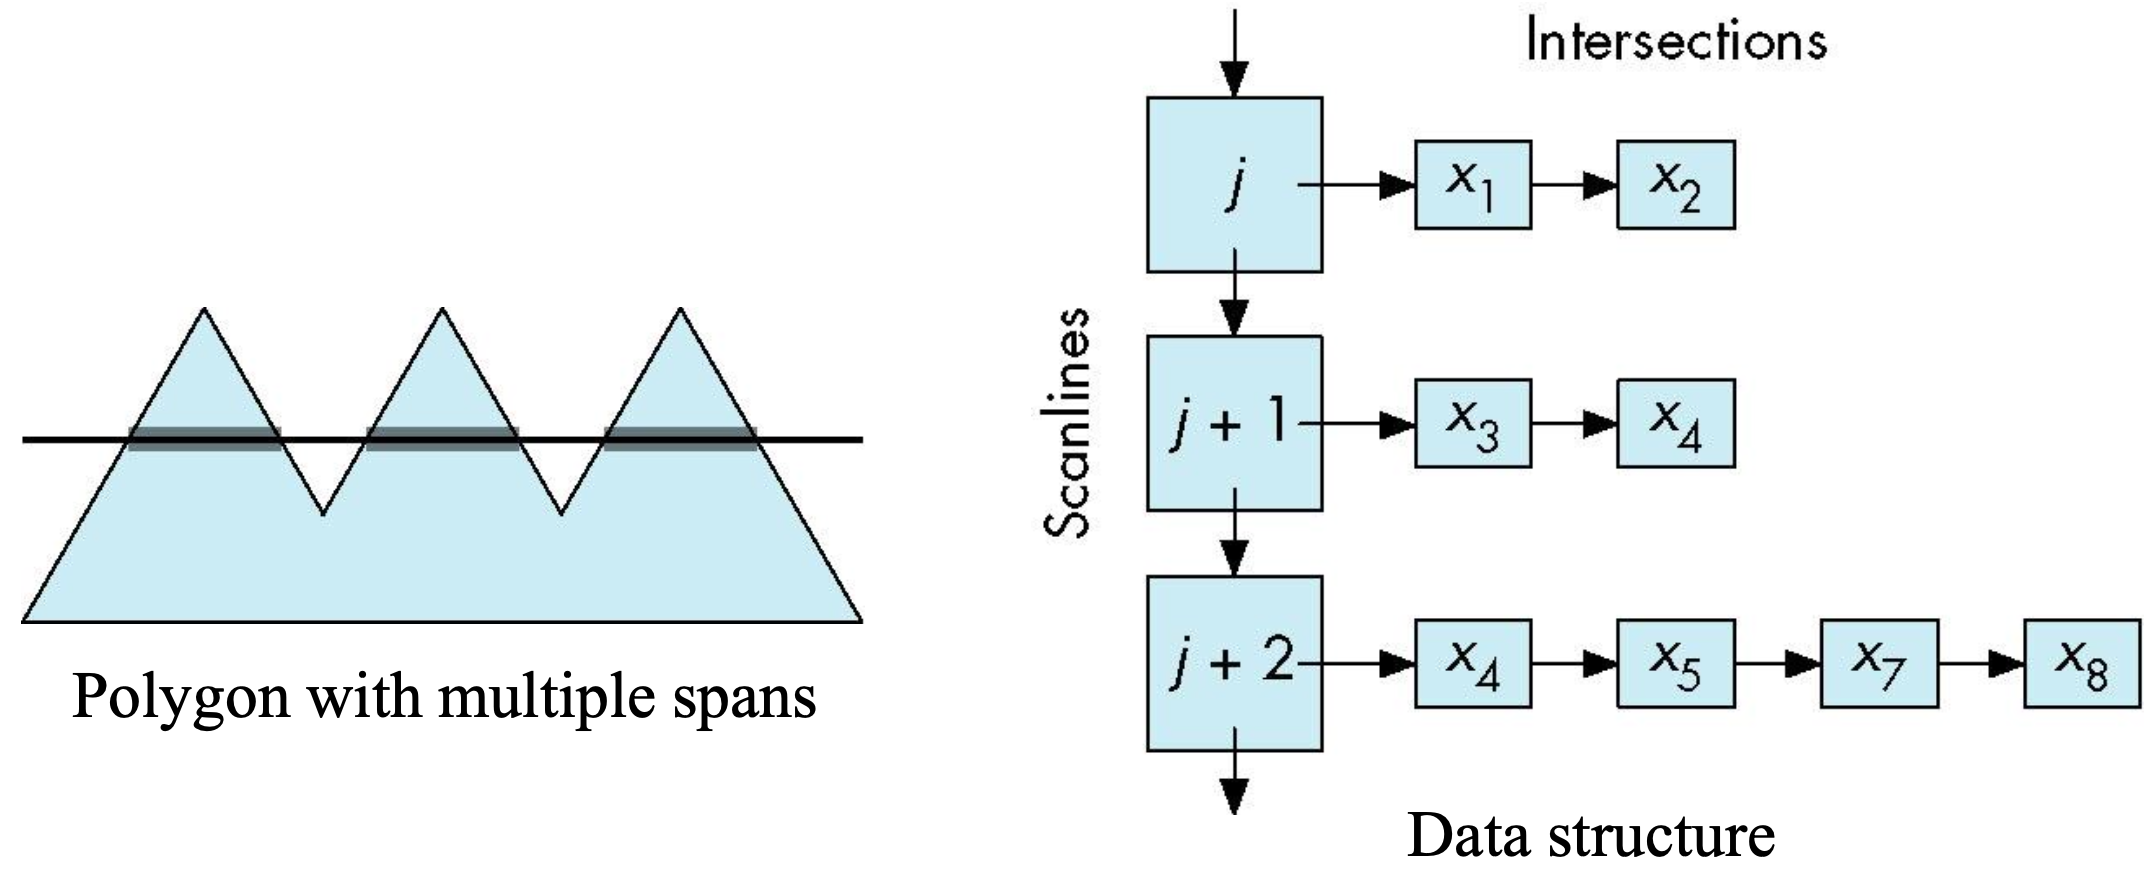
\includegraphics[width=\columnwidth]{L6/scan-line-ds}
  \subsection*{Flood-fill}
    \begin{itemize}[leftmargin=*]
      \item Fill can be done recursively if we know a seed point located inside
      \item But first scan-convert edges using an edge color
    \end{itemize}
\section*{\normalsize	Hidden-surface removal}
    \begin{itemize}[leftmargin=*]
      \item In 3D graphics, some object should appear in front of another
      \item Without hidden-surface removal, objects ``on top'' are the ones that are drawn last
      \item Hidden-surface removal fixes this problem using the z-buffer algorithm
    \end{itemize}
  \subsection*{Painter's algorithm (Depth sorting)}
    \begin{itemize}[leftmargin=*]
      \item Render polygons in back-to-front order so that polygons behind others are simply painted over
      \item Depth-sorting can be done in $O(n \log n)$ time
      \item Cannot handle cyclic overlap of polygons
        \begin{itemize}[leftmargin=*]
          \item Solution: split original polygons
        \end{itemize}
    \end{itemize}
    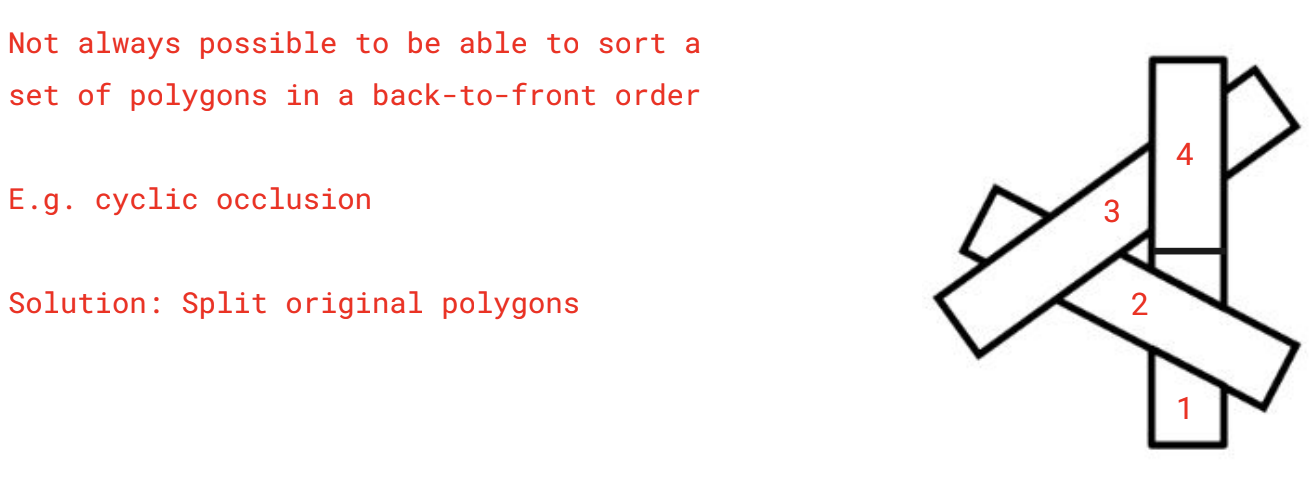
\includegraphics[width=\columnwidth]{L6/cyclic-occlusion}
  \subsection*{Back-face culling}
    \begin{itemize}[leftmargin=*]
      \item Eliminate polygon if it is back-facing and invisible (e.g. back face of a 3d building)
      \item It is back facing if $N_p \cdot N < 0$
    \end{itemize}
    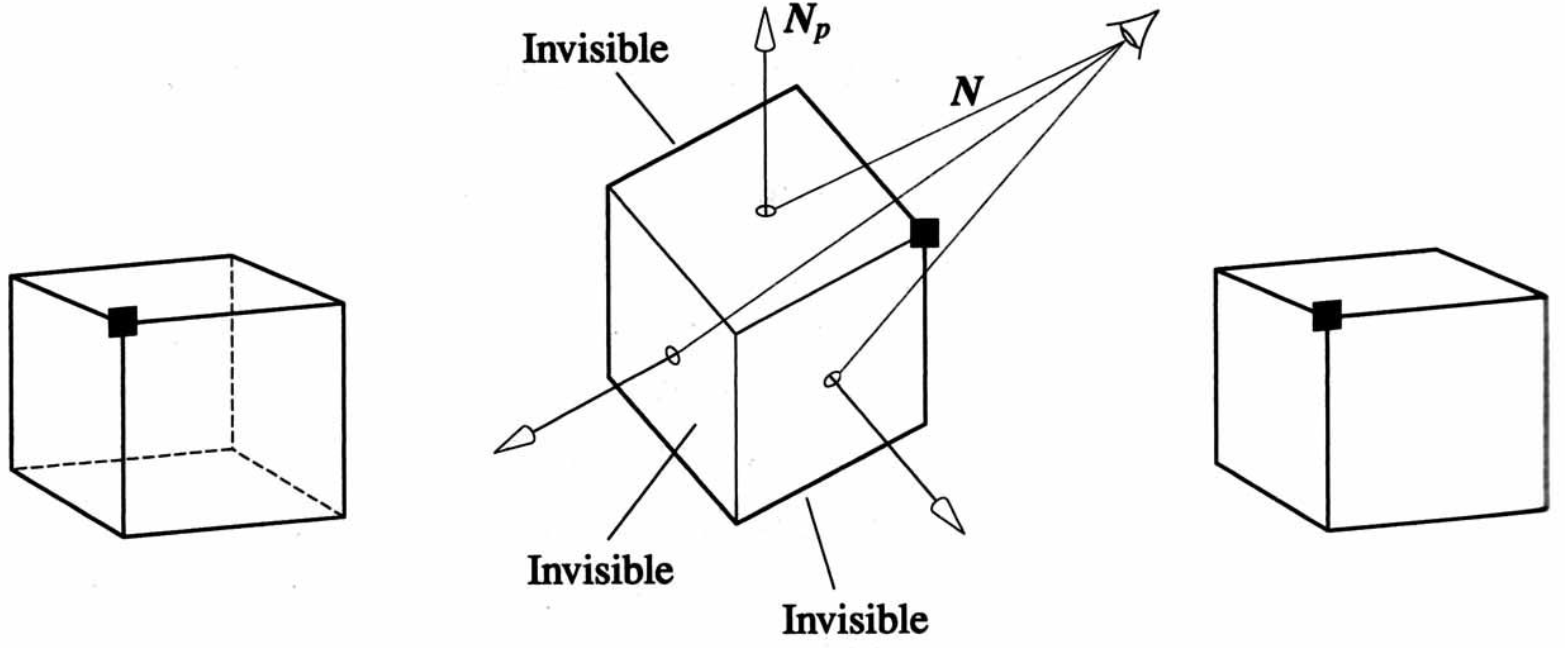
\includegraphics[width=\columnwidth]{L6/back-face-culling}
    \begin{itemize}[leftmargin=*]
      \item In OpenGL, simply enable culling
        \begin{itemize}[leftmargin=*]
          \item Polygon vertices must be provided in counter-clockwise order
          \item May not work correctly for non-convex polygon
        \end{itemize}
    \end{itemize}
  \subsection*{Image space approach}
    \begin{itemize}[leftmargin=*]
      \item For each projector ($nm$ projectors for a $n$ by $m$ frame buffer), find the closest polygon among $k$ polygons
      \item $O(nmk)$
      \item e.g. Ray tracing, $z$-buffer
    \end{itemize}
    \subsubsection*{$z$-buffer algorithm}
      \begin{itemize}[leftmargin=*]
        \item Use a $z$-buffer or depth buffer to store depth of closest object at each pixel so far
        \item As we render each polygon, compare depth of each fragment, to depth in $z$-buffer
        \item If less than, update, placing fragment in color buffer and its depth in $z$-buffer
        \item If not, then discard
      \end{itemize}
      \paragraph{Usage}
        \begin{lstlisting}
// In main()
glutInitDisplayMode(... | GLUT_DEPTH);
// In init()
glEnable(GL_DEPTH_TEST);
// Cleared in display callback
glClear(... | GL_DEPTH_BUFFER_BIT);
        \end{lstlisting}
\end{multicols*}
\begin{multicols}{2}
\section*{Tutorials}
  \vspace{-0.5cm}
  \subsection*{T2 Q7}
    \vspace{-0.5cm}
    \subsubsection*{Question} \noindent
      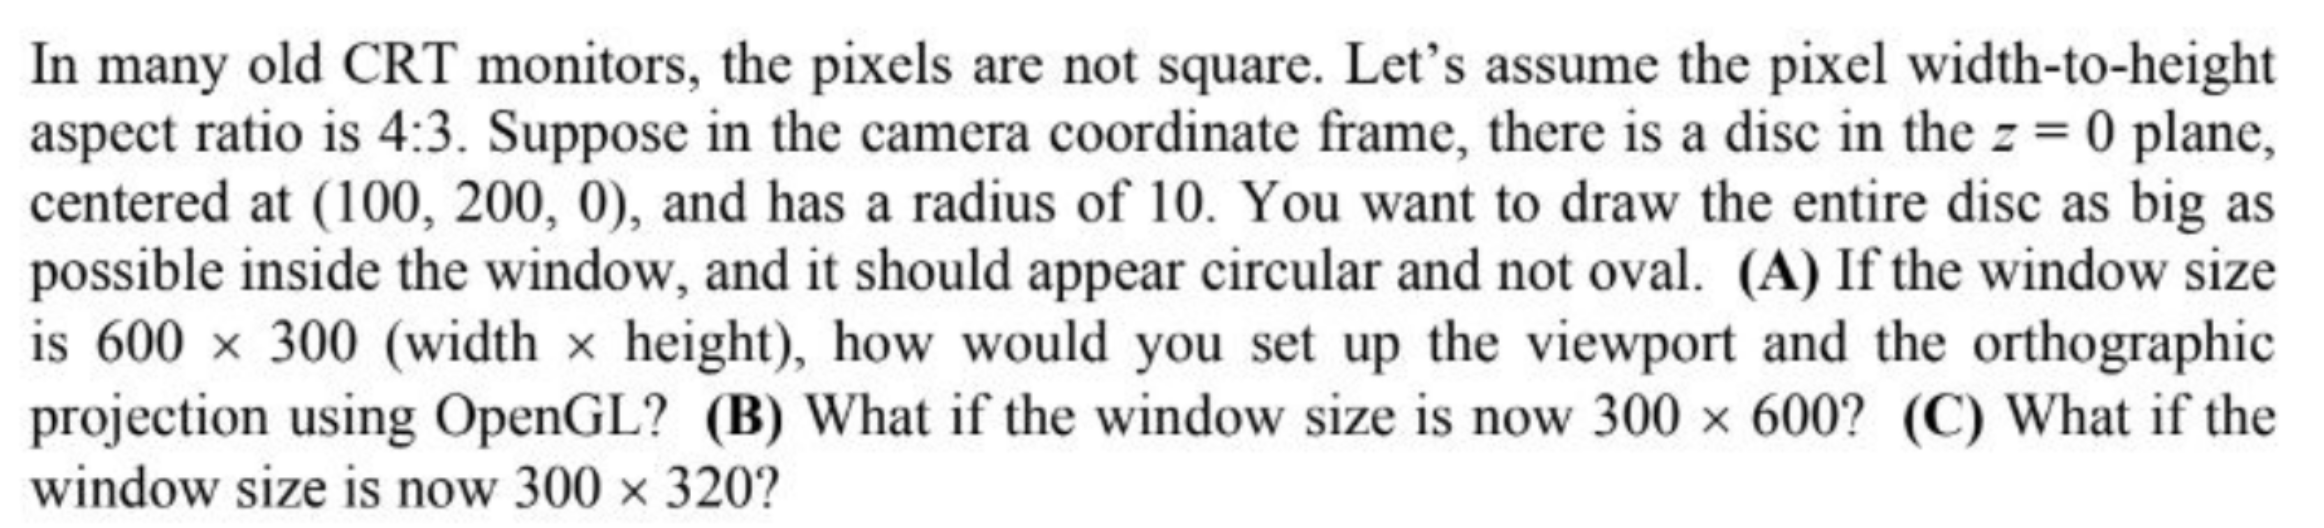
\includegraphics[width=\columnwidth]{T2/Q7}
    \subsubsection*{Answer} \noindent
      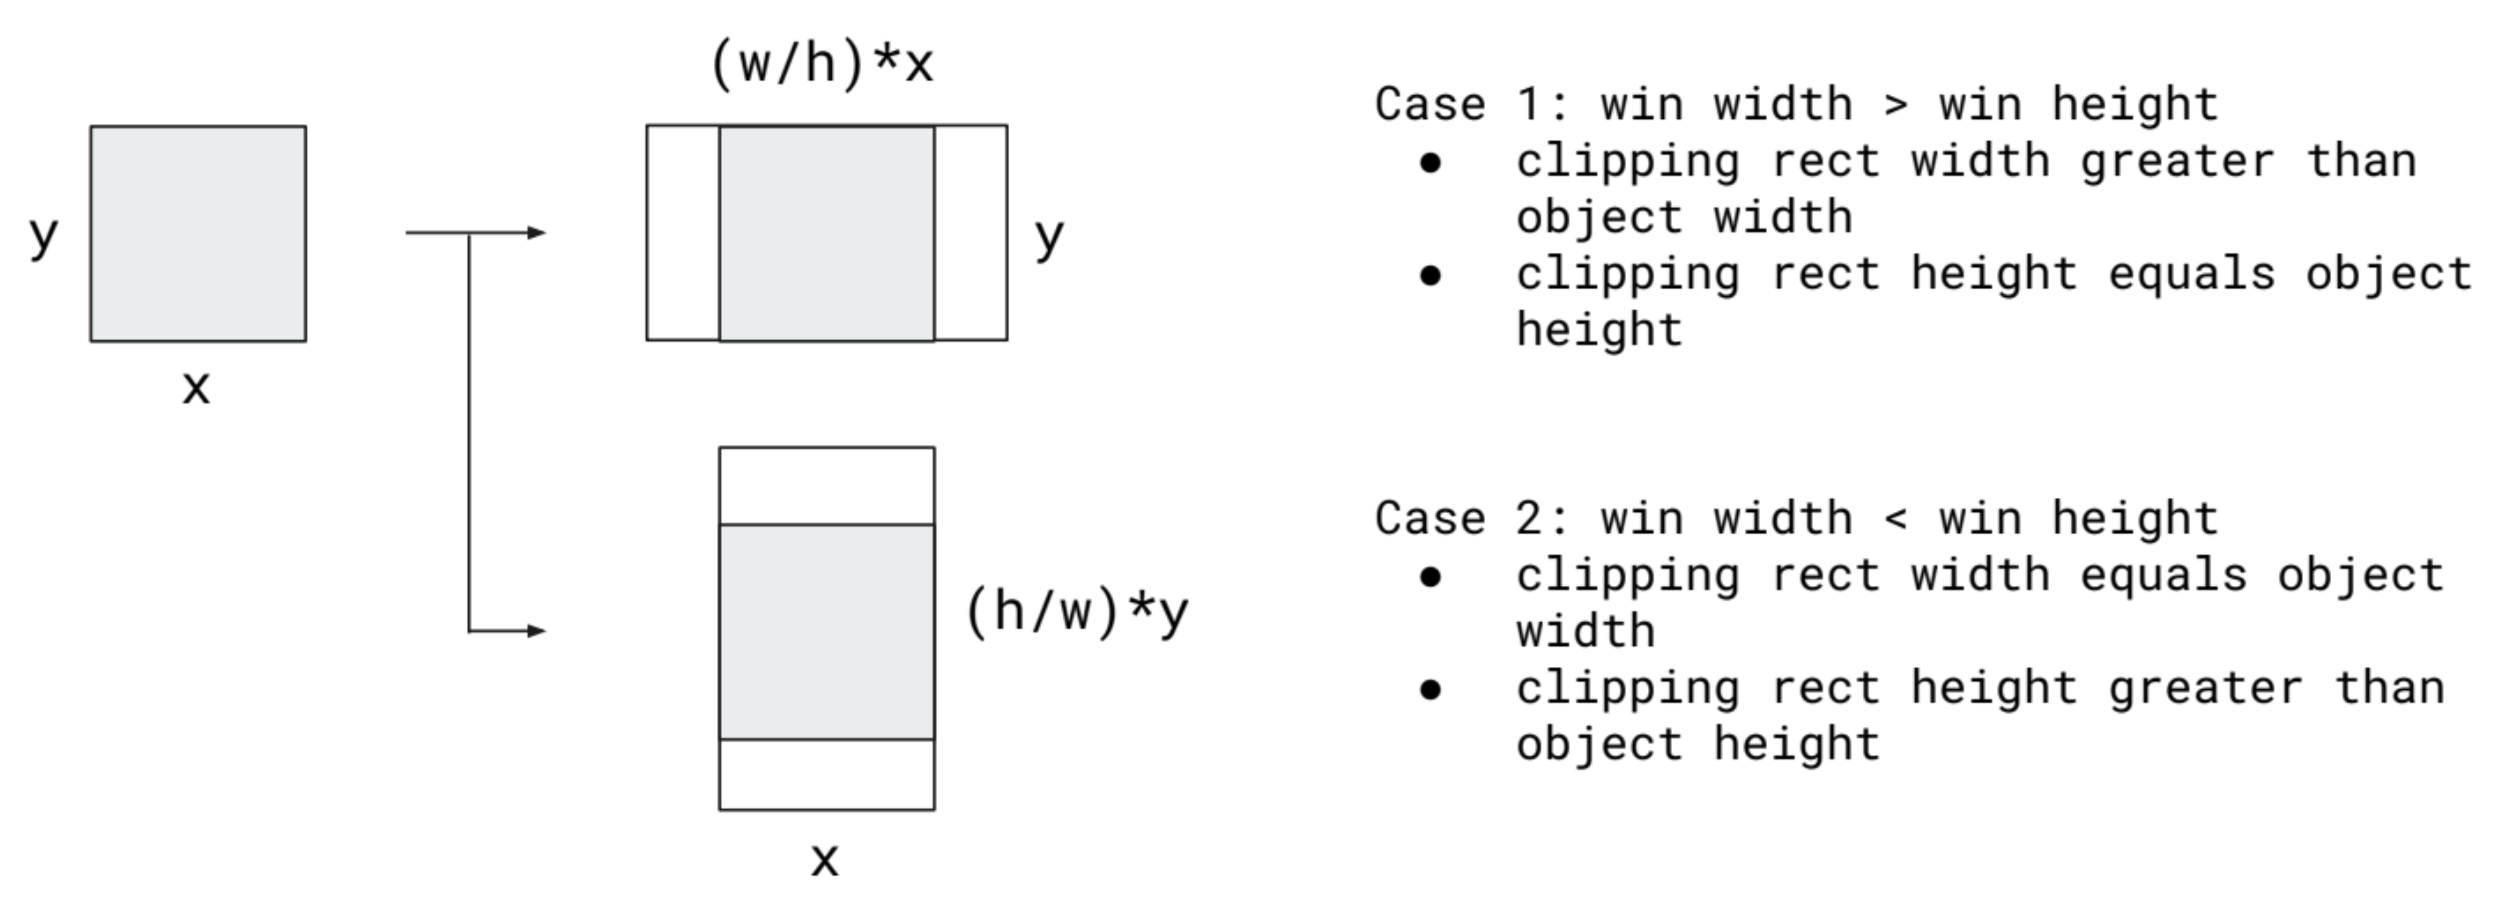
\includegraphics[width=\columnwidth]{T2/Q7-idea}
      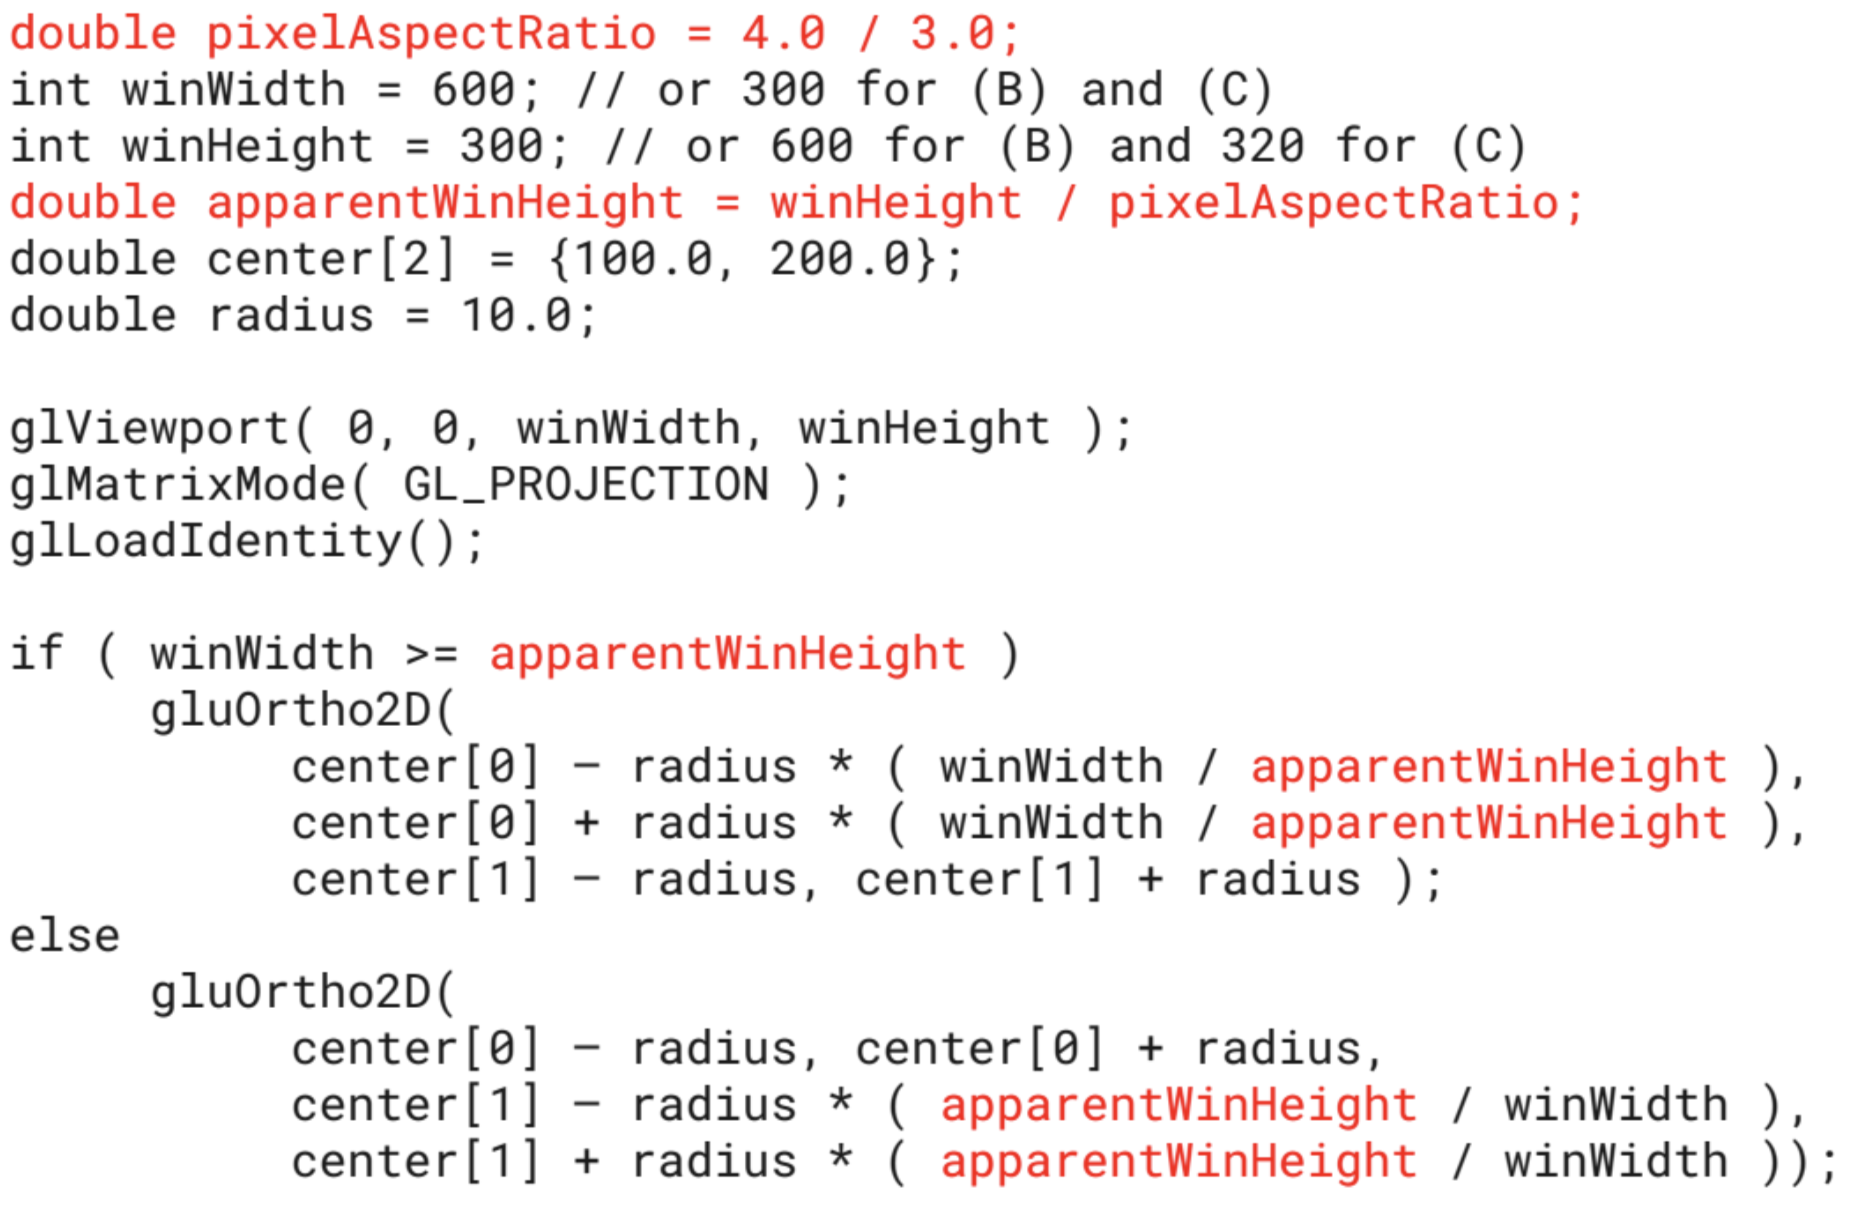
\includegraphics[width=\columnwidth]{T2/Q7-code}
  \subsection*{T4 Q3} \noindent
    \vspace{-0.5cm}
    \begin{itemize}[leftmargin=*]
      \item By convention we use a right-handed coordinate system
      \item The right thumb points along the z axis in the positive direction and the curl of the fingers represents a motion from the first or x axis to the second or y axis
      \item Alternatively, thumb points at $x$, pointer points at $y$, middle finger points at $z$ (left image below)
    \end{itemize}
    \begin{center}
      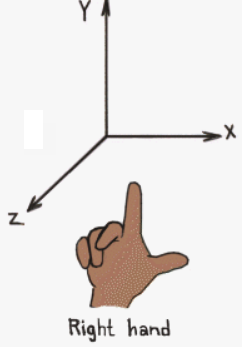
\includegraphics[width=0.3\columnwidth]{T4/right-handed}
      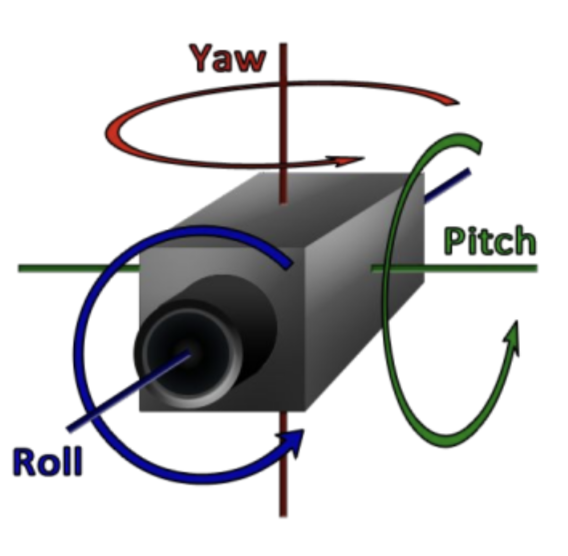
\includegraphics[width=0.45\columnwidth]{T4/rotation}
    \end{center}
    \begin{hlist}
      \item Pitch: rotation about $x$-axis
      \item Yaw: rotation about $y$-axis
      \item Roll: rotation about $z$-axis
    \end{hlist}
\columnbreak
  \subsection*{T3 Q1c}
    \vspace{-0.5cm}
    \subsubsection*{Projection of a onto b} \noindent
      \vspace{-0.7cm}
      \begin{center}
        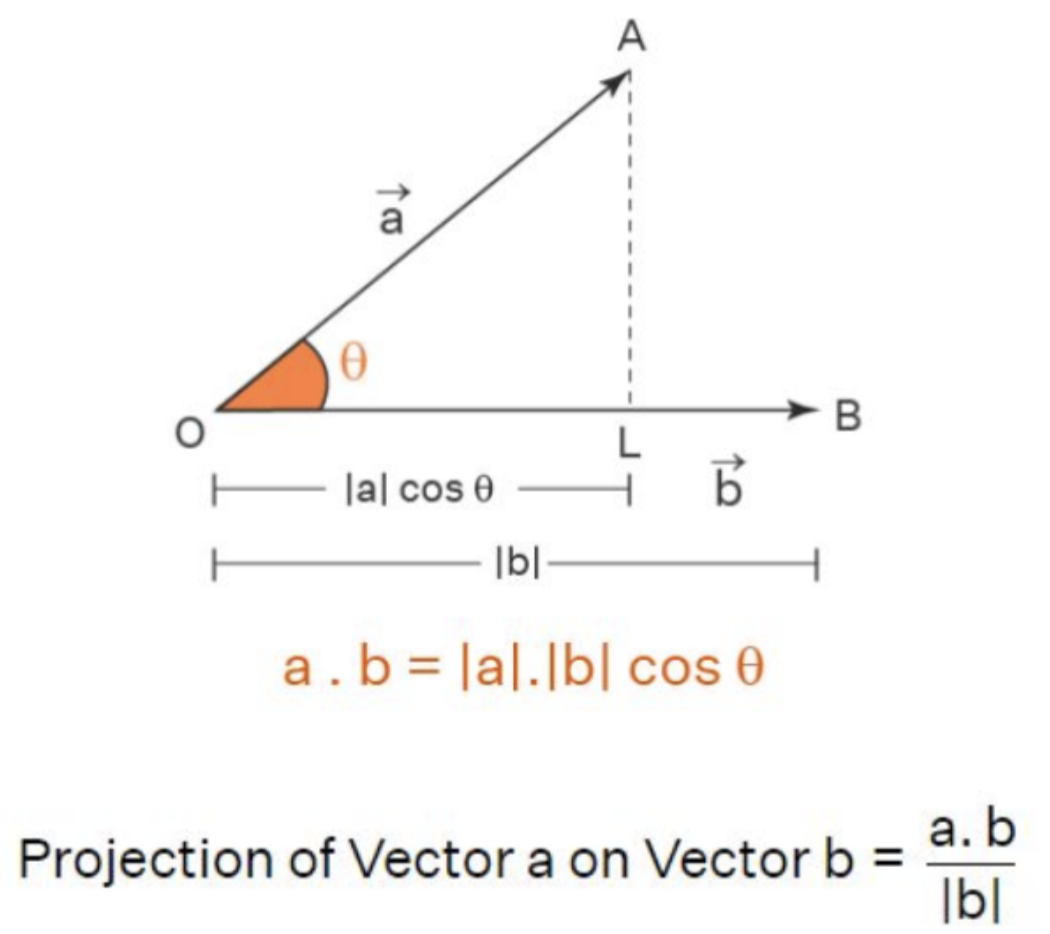
\includegraphics[width=0.5\columnwidth]{T3/projection}
      \end{center}
    \subsubsection*{Perpendicular distance of point $Q$ to a plane} \noindent
      Let plane be defined as $ax + by + cz + d = 0$. The perpendicular distance from $Q$ to the plane is given by
      \[ \frac{\lvert ax_q + by_q + cz_q + d \rvert}{\sqrt{a^2 + b^2 + c^2}} \]
      Proof: \\
      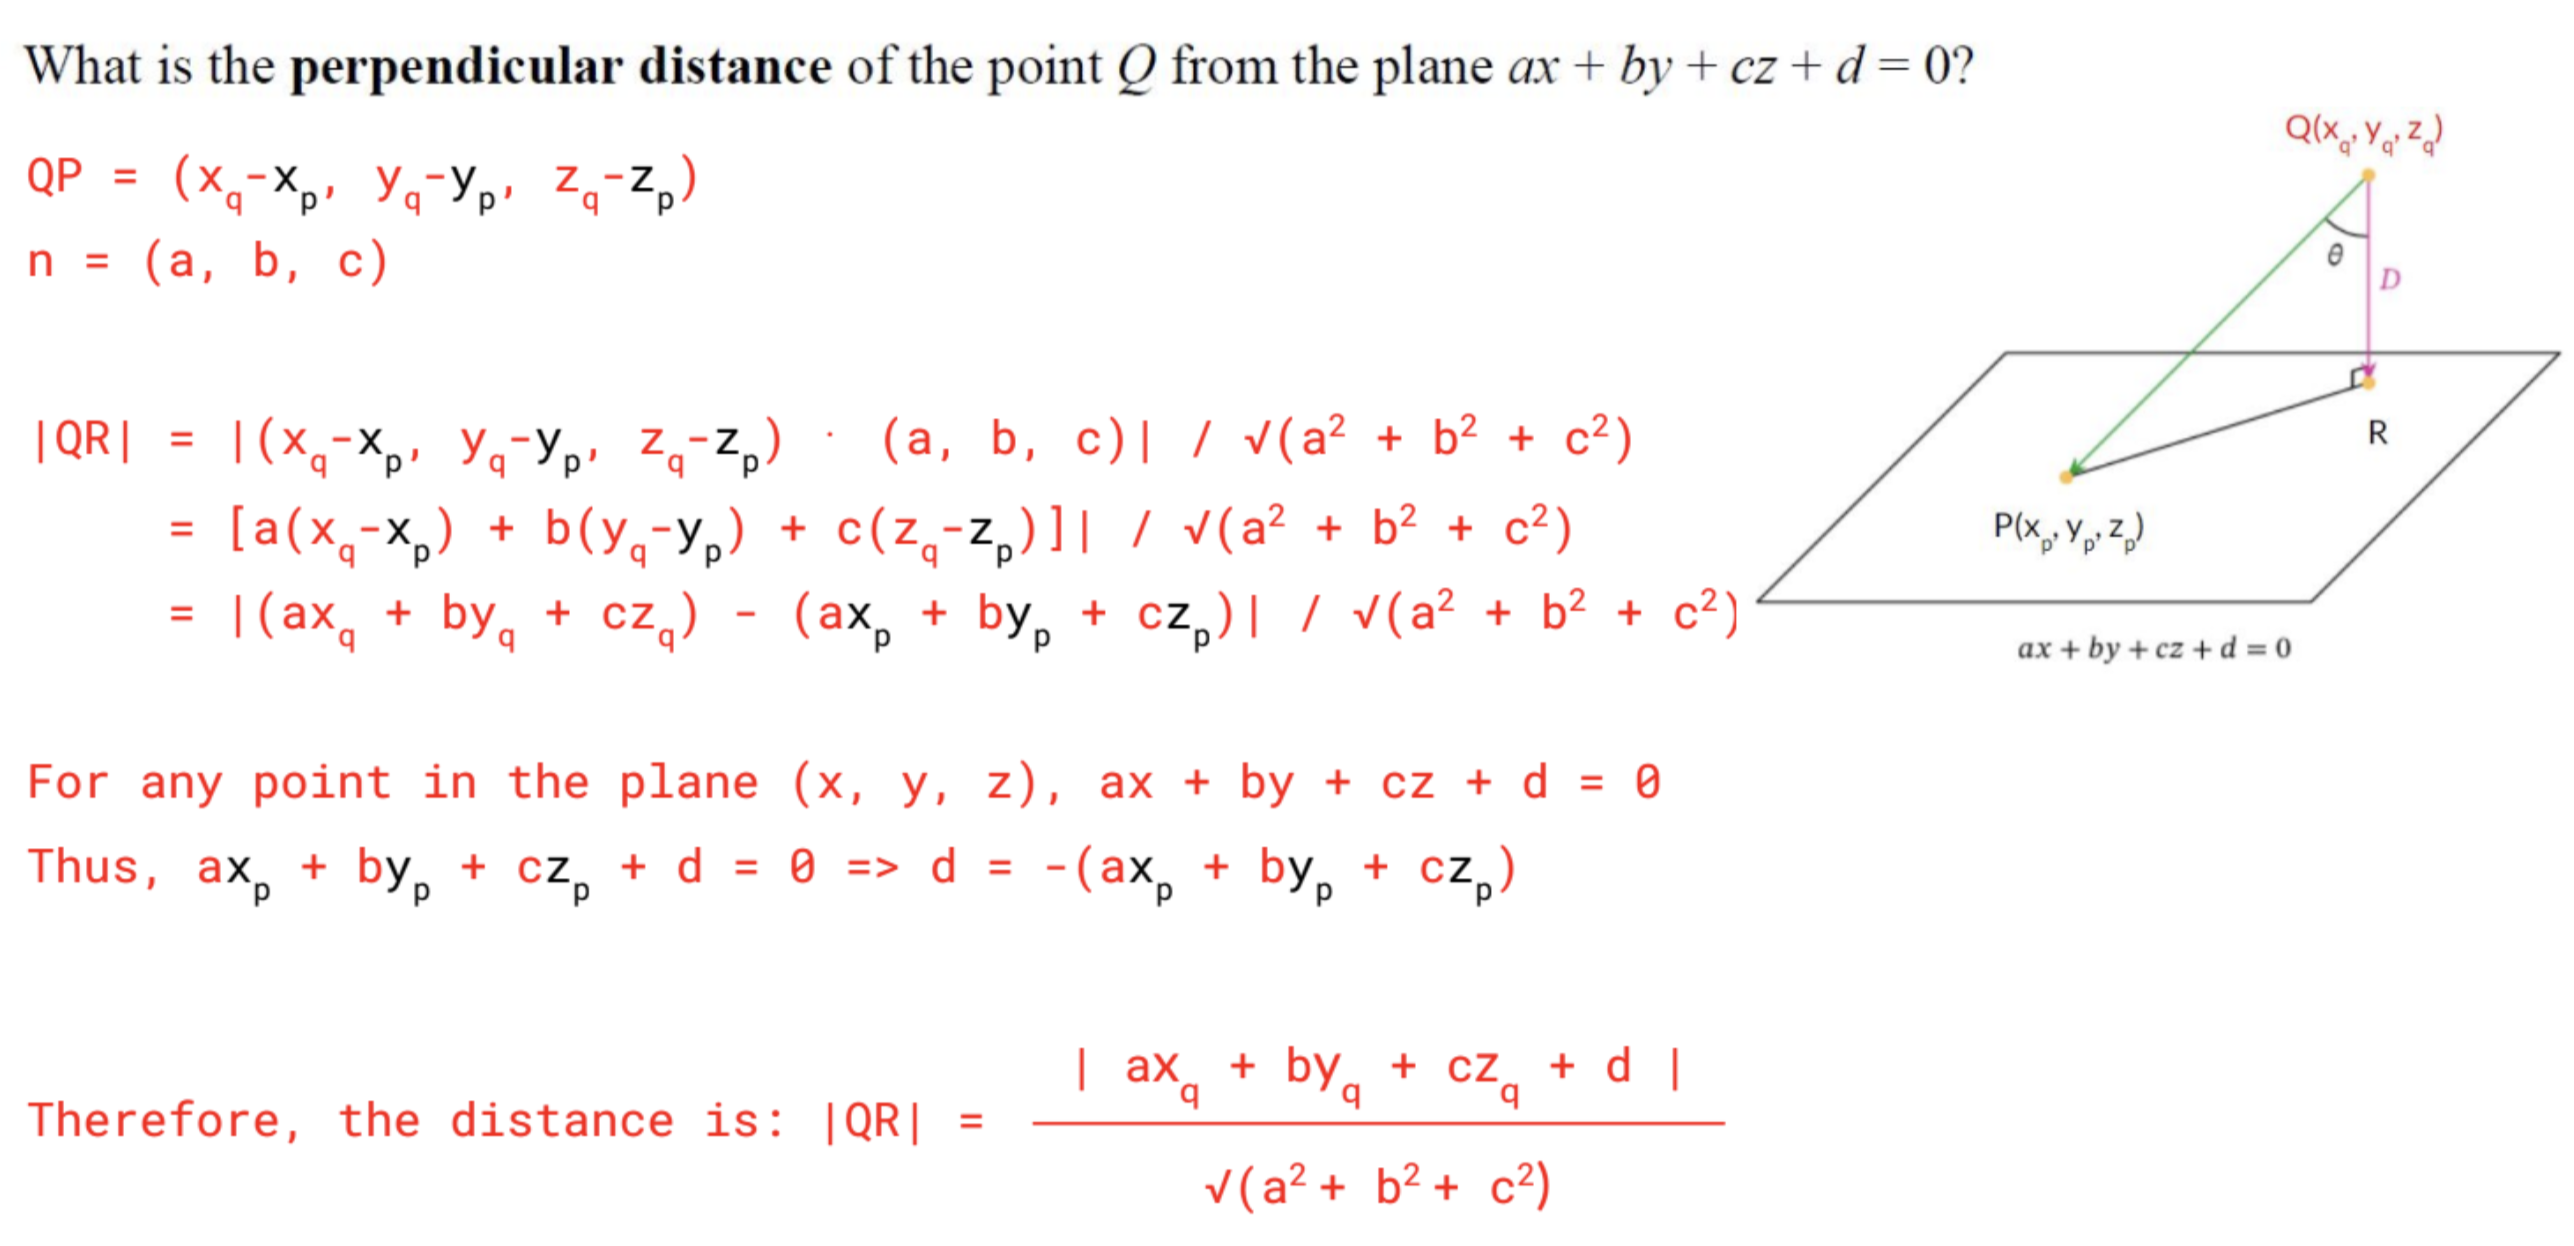
\includegraphics[width=\columnwidth]{T3/perpendicular-distance}
    \vspace{-0.5cm}
  \subsection*{T3 Q4} \noindent
    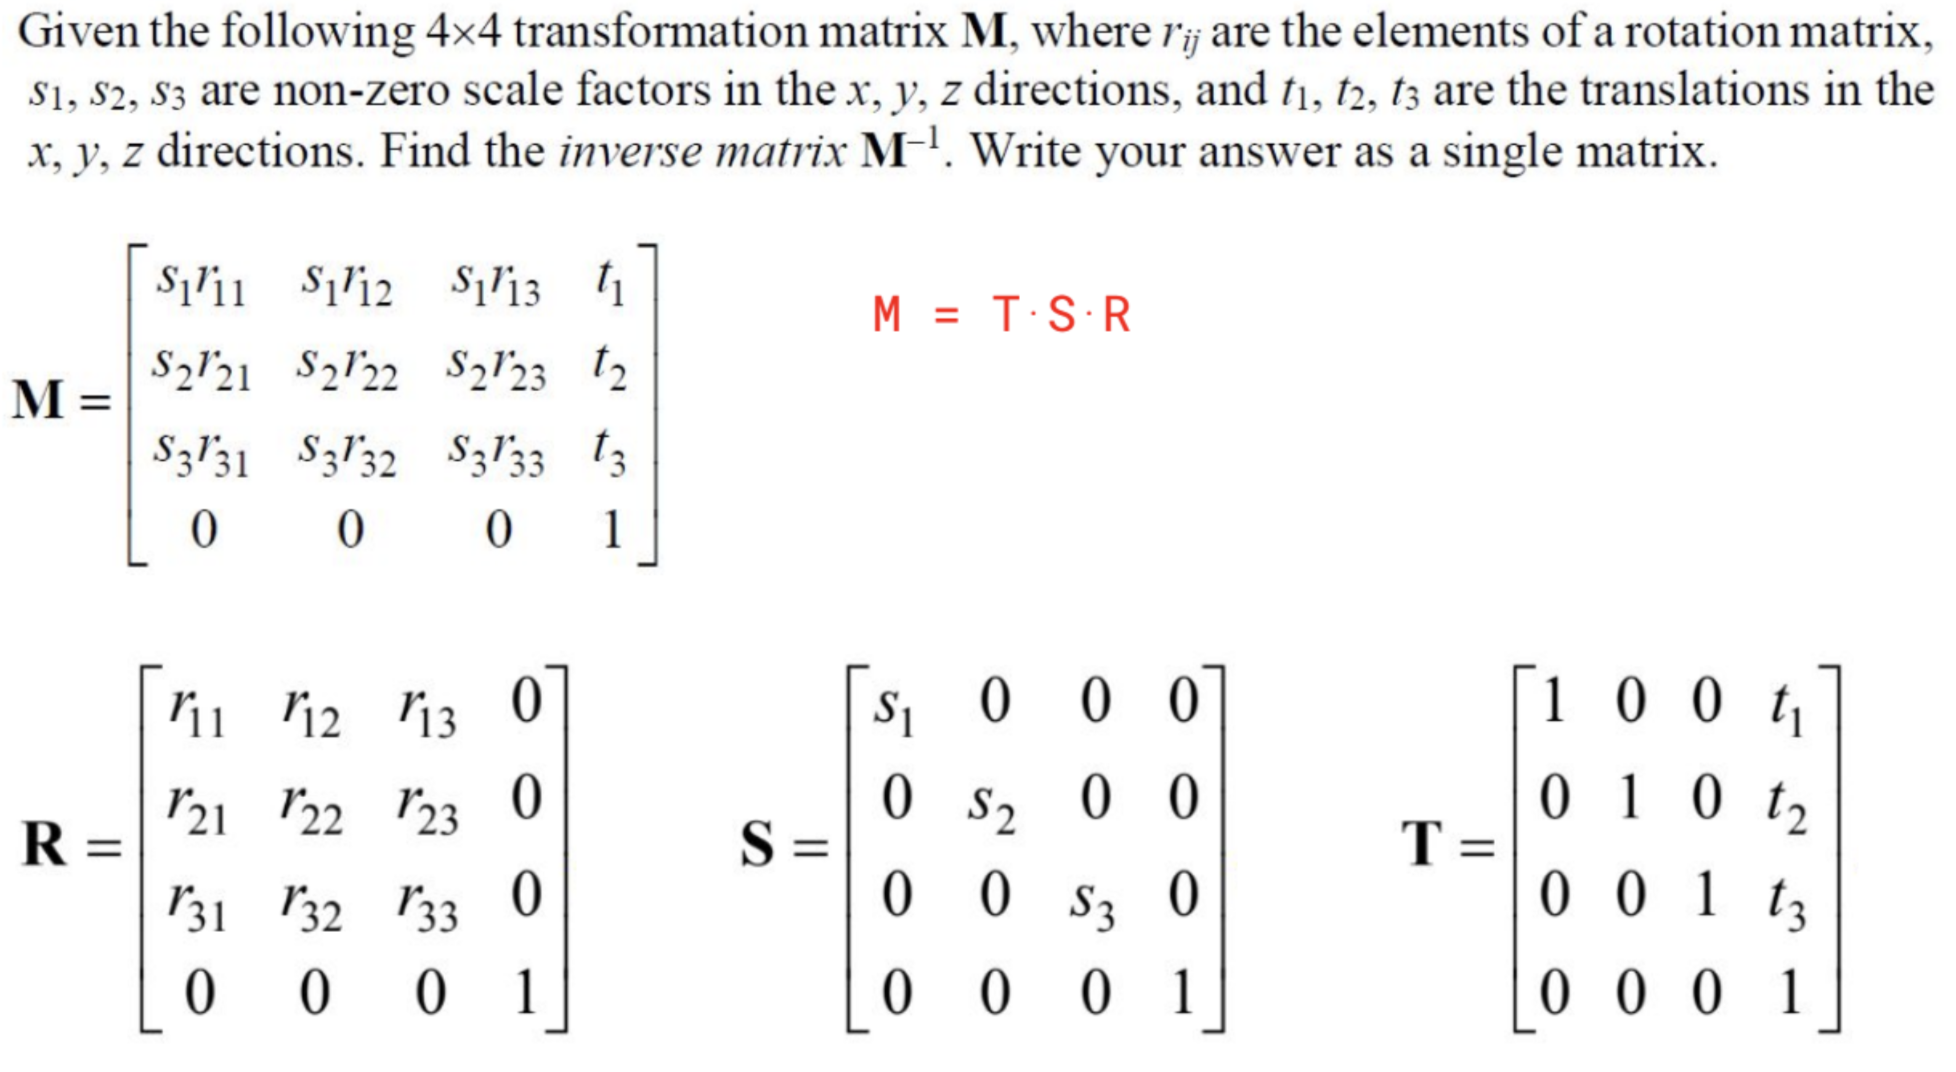
\includegraphics[width=\columnwidth]{T3/Q4}
    \begin{itemize}[leftmargin=*]
      \item Clearly $T$ is applied last, since you can reverse the translation and get a clean matrix
      \item Then, $S$ is applied after $R$ because $s_1$ is distributed along the row
    \end{itemize}
  \subsection*{T4 Q5} \noindent
    \vspace{-0.5cm}
    \begin{itemize}[leftmargin=*]
      \item To convert from camera coordinates to NDC, notice that the ratio of the vertex along each axis stays the same after the transformation
    \end{itemize}
    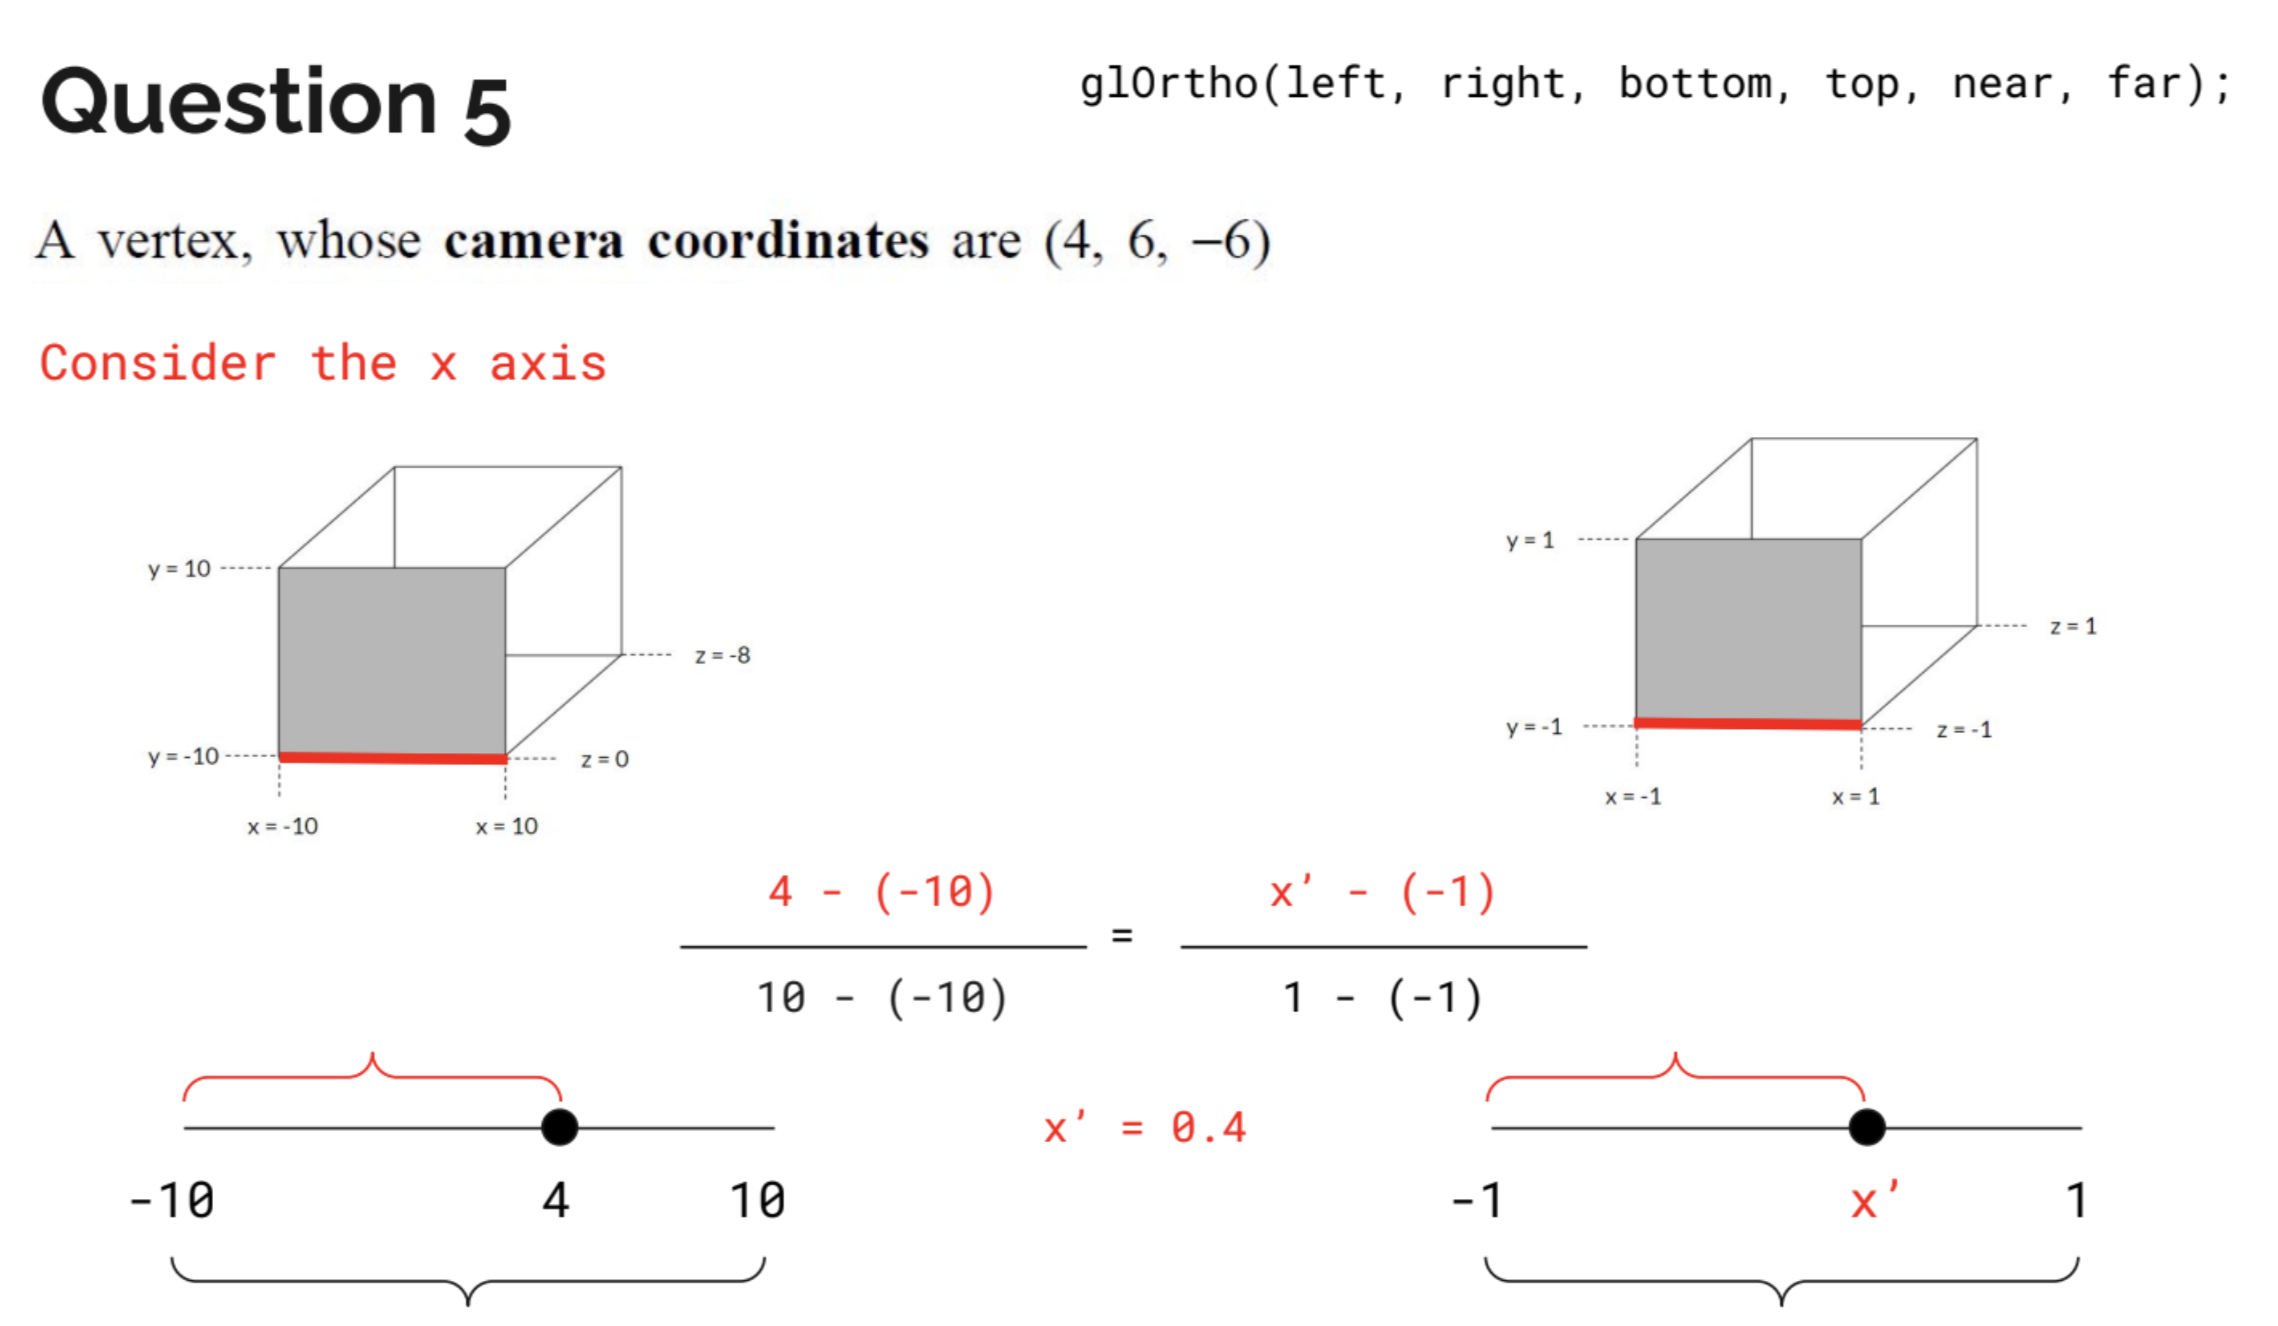
\includegraphics[width=\columnwidth]{T4/convert-to-NDC}
\end{multicols}
\end{document}
